\documentclass[twoside]{book}

% Packages required by doxygen
\usepackage{fixltx2e}
\usepackage{calc}
\usepackage{doxygen}
\usepackage[export]{adjustbox} % also loads graphicx
\usepackage{graphicx}
\usepackage[utf8]{inputenc}
\usepackage{makeidx}
\usepackage{multicol}
\usepackage{multirow}
\PassOptionsToPackage{warn}{textcomp}
\usepackage{textcomp}
\usepackage[nointegrals]{wasysym}
\usepackage[table]{xcolor}

% Font selection
\usepackage[T1]{fontenc}
\usepackage[scaled=.90]{helvet}
\usepackage{courier}
\usepackage{amssymb}
\usepackage{sectsty}
\renewcommand{\familydefault}{\sfdefault}
\allsectionsfont{%
  \fontseries{bc}\selectfont%
  \color{darkgray}%
}
\renewcommand{\DoxyLabelFont}{%
  \fontseries{bc}\selectfont%
  \color{darkgray}%
}
\newcommand{\+}{\discretionary{\mbox{\scriptsize$\hookleftarrow$}}{}{}}

% Page & text layout
\usepackage{geometry}
\geometry{%
  a4paper,%
  top=2.5cm,%
  bottom=2.5cm,%
  left=2.5cm,%
  right=2.5cm%
}
\tolerance=750
\hfuzz=15pt
\hbadness=750
\setlength{\emergencystretch}{15pt}
\setlength{\parindent}{0cm}
\setlength{\parskip}{3ex plus 2ex minus 2ex}
\makeatletter
\renewcommand{\paragraph}{%
  \@startsection{paragraph}{4}{0ex}{-1.0ex}{1.0ex}{%
    \normalfont\normalsize\bfseries\SS@parafont%
  }%
}
\renewcommand{\subparagraph}{%
  \@startsection{subparagraph}{5}{0ex}{-1.0ex}{1.0ex}{%
    \normalfont\normalsize\bfseries\SS@subparafont%
  }%
}
\makeatother

% Headers & footers
\usepackage{fancyhdr}
\pagestyle{fancyplain}
\fancyhead[LE]{\fancyplain{}{\bfseries\thepage}}
\fancyhead[CE]{\fancyplain{}{}}
\fancyhead[RE]{\fancyplain{}{\bfseries\leftmark}}
\fancyhead[LO]{\fancyplain{}{\bfseries\rightmark}}
\fancyhead[CO]{\fancyplain{}{}}
\fancyhead[RO]{\fancyplain{}{\bfseries\thepage}}
\fancyfoot[LE]{\fancyplain{}{}}
\fancyfoot[CE]{\fancyplain{}{}}
\fancyfoot[RE]{\fancyplain{}{\bfseries\scriptsize Generated by Doxygen }}
\fancyfoot[LO]{\fancyplain{}{\bfseries\scriptsize Generated by Doxygen }}
\fancyfoot[CO]{\fancyplain{}{}}
\fancyfoot[RO]{\fancyplain{}{}}
\renewcommand{\footrulewidth}{0.4pt}
\renewcommand{\chaptermark}[1]{%
  \markboth{#1}{}%
}
\renewcommand{\sectionmark}[1]{%
  \markright{\thesection\ #1}%
}

% Indices & bibliography
\usepackage{natbib}
\usepackage[titles]{tocloft}
\setcounter{tocdepth}{3}
\setcounter{secnumdepth}{5}
\makeindex

% Hyperlinks (required, but should be loaded last)
\usepackage{ifpdf}
\ifpdf
  \usepackage[pdftex,pagebackref=true]{hyperref}
\else
  \usepackage[ps2pdf,pagebackref=true]{hyperref}
\fi
\hypersetup{%
  colorlinks=true,%
  linkcolor=blue,%
  citecolor=blue,%
  unicode%
}

% Custom commands
\newcommand{\clearemptydoublepage}{%
  \newpage{\pagestyle{empty}\cleardoublepage}%
}

\usepackage{caption}
\captionsetup{labelsep=space,justification=centering,font={bf},singlelinecheck=off,skip=4pt,position=top}

%===== C O N T E N T S =====

\begin{document}

% Titlepage & ToC
\hypersetup{pageanchor=false,
             bookmarksnumbered=true,
             pdfencoding=unicode
            }
\pagenumbering{alph}
\begin{titlepage}
\vspace*{7cm}
\begin{center}%
{\Large My Project }\\
\vspace*{1cm}
{\large Generated by Doxygen 1.8.14}\\
\end{center}
\end{titlepage}
\clearemptydoublepage
\pagenumbering{roman}
\tableofcontents
\clearemptydoublepage
\pagenumbering{arabic}
\hypersetup{pageanchor=true}

%--- Begin generated contents ---
\chapter{Main Page}
\label{index}\hypertarget{index}{}\begin{DoxyParagraph}{Symulacja robotów mobilnych}
Program ma za zadanie symulować zachowanie różnych typów robotów mobilnych poruszających się po planszy i wykonujących różne zadania. 
\end{DoxyParagraph}
\begin{DoxyAuthor}{Author}
Filip Szatkowski 
\end{DoxyAuthor}
\begin{DoxyDate}{Date}
13.\+06.\+2018 
\end{DoxyDate}

\chapter{Hierarchical Index}
\section{Class Hierarchy}
This inheritance list is sorted roughly, but not completely, alphabetically\+:\begin{DoxyCompactList}
\item \contentsline{section}{C\+Map}{\pageref{class_c_map}}{}
\item \contentsline{section}{C\+Object}{\pageref{class_c_object}}{}
\begin{DoxyCompactList}
\item \contentsline{section}{C\+Movable}{\pageref{class_c_movable}}{}
\begin{DoxyCompactList}
\item \contentsline{section}{C\+Bullet}{\pageref{class_c_bullet}}{}
\item \contentsline{section}{C\+Obstacle}{\pageref{class_c_obstacle}}{}
\item \contentsline{section}{C\+Robot}{\pageref{class_c_robot}}{}
\begin{DoxyCompactList}
\item \contentsline{section}{C\+Cleaning\+Robot}{\pageref{class_c_cleaning_robot}}{}
\item \contentsline{section}{C\+Fighting\+Robot}{\pageref{class_c_fighting_robot}}{}
\item \contentsline{section}{C\+Searching\+Robot}{\pageref{class_c_searching_robot}}{}
\end{DoxyCompactList}
\end{DoxyCompactList}
\item \contentsline{section}{C\+Non\+Movable}{\pageref{class_c_non_movable}}{}
\begin{DoxyCompactList}
\item \contentsline{section}{C\+Dirt}{\pageref{class_c_dirt}}{}
\item \contentsline{section}{C\+Mine}{\pageref{class_c_mine}}{}
\item \contentsline{section}{C\+Treasure}{\pageref{class_c_treasure}}{}
\end{DoxyCompactList}
\end{DoxyCompactList}
\item Q\+Graphics\+Item\begin{DoxyCompactList}
\item \contentsline{section}{C\+G\+Object}{\pageref{class_c_g_object}}{}
\begin{DoxyCompactList}
\item \contentsline{section}{C\+G\+Bullet}{\pageref{class_c_g_bullet}}{}
\item \contentsline{section}{C\+G\+Cleaning\+Robot}{\pageref{class_c_g_cleaning_robot}}{}
\item \contentsline{section}{C\+G\+Dirt}{\pageref{class_c_g_dirt}}{}
\item \contentsline{section}{C\+G\+Fighting\+Robot}{\pageref{class_c_g_fighting_robot}}{}
\item \contentsline{section}{C\+G\+Mine}{\pageref{class_c_g_mine}}{}
\item \contentsline{section}{C\+G\+Obstacle}{\pageref{class_c_g_obstacle}}{}
\item \contentsline{section}{C\+G\+Searching\+Robot}{\pageref{class_c_g_searching_robot}}{}
\item \contentsline{section}{C\+G\+Treasure}{\pageref{class_c_g_treasure}}{}
\end{DoxyCompactList}
\end{DoxyCompactList}
\item Q\+Widget\begin{DoxyCompactList}
\item \contentsline{section}{C\+Program}{\pageref{class_c_program}}{}
\end{DoxyCompactList}
\end{DoxyCompactList}

\chapter{Class Index}
\section{Class List}
Here are the classes, structs, unions and interfaces with brief descriptions\+:\begin{DoxyCompactList}
\item\contentsline{section}{\mbox{\hyperlink{class_c_bullet}{C\+Bullet}} \\*Pociski wystrzeliwywane przez roboty walczące }{\pageref{class_c_bullet}}{}
\item\contentsline{section}{\mbox{\hyperlink{class_c_cleaning_robot}{C\+Cleaning\+Robot}} \\*Robot zajmujący się sprzątaniem brudów z mapy }{\pageref{class_c_cleaning_robot}}{}
\item\contentsline{section}{\mbox{\hyperlink{class_c_dirt}{C\+Dirt}} \\*Brudy zbierane przez roboty sprzątające }{\pageref{class_c_dirt}}{}
\item\contentsline{section}{\mbox{\hyperlink{class_c_fighting_robot}{C\+Fighting\+Robot}} \\*Robot atakujący inne roboty }{\pageref{class_c_fighting_robot}}{}
\item\contentsline{section}{\mbox{\hyperlink{class_c_g_bullet}{C\+G\+Bullet}} \\*Graficzna reprezentacja pocisku }{\pageref{class_c_g_bullet}}{}
\item\contentsline{section}{\mbox{\hyperlink{class_c_g_cleaning_robot}{C\+G\+Cleaning\+Robot}} \\*Graficzna reprezentacja robota czyszczącego }{\pageref{class_c_g_cleaning_robot}}{}
\item\contentsline{section}{\mbox{\hyperlink{class_c_g_dirt}{C\+G\+Dirt}} \\*Graficzna reprezentacja brudu }{\pageref{class_c_g_dirt}}{}
\item\contentsline{section}{\mbox{\hyperlink{class_c_g_fighting_robot}{C\+G\+Fighting\+Robot}} \\*Graficzna reprezentacja robota walczącego }{\pageref{class_c_g_fighting_robot}}{}
\item\contentsline{section}{\mbox{\hyperlink{class_c_g_mine}{C\+G\+Mine}} \\*Graficzna reprezentacja miny }{\pageref{class_c_g_mine}}{}
\item\contentsline{section}{\mbox{\hyperlink{class_c_g_object}{C\+G\+Object}} \\*Klasa służąca do wyświetlania na mapie obiektów logicznych }{\pageref{class_c_g_object}}{}
\item\contentsline{section}{\mbox{\hyperlink{class_c_g_obstacle}{C\+G\+Obstacle}} \\*Graficzna reprezentacja przeszkody }{\pageref{class_c_g_obstacle}}{}
\item\contentsline{section}{\mbox{\hyperlink{class_c_g_searching_robot}{C\+G\+Searching\+Robot}} \\*Graficzna reprezentacja robota szukającego }{\pageref{class_c_g_searching_robot}}{}
\item\contentsline{section}{\mbox{\hyperlink{class_c_g_treasure}{C\+G\+Treasure}} \\*Graficzna reprezentacja skarbu }{\pageref{class_c_g_treasure}}{}
\item\contentsline{section}{\mbox{\hyperlink{class_c_map}{C\+Map}} \\*Mapa, na której poruszają się wszystkie obiekty }{\pageref{class_c_map}}{}
\item\contentsline{section}{\mbox{\hyperlink{class_c_mine}{C\+Mine}} \\*Mina niszcząca roboty, które na nią wpadną }{\pageref{class_c_mine}}{}
\item\contentsline{section}{\mbox{\hyperlink{class_c_movable}{C\+Movable}} \\*Klasa reprezentująca obiekty z możliwością poruszania się po mapie }{\pageref{class_c_movable}}{}
\item\contentsline{section}{\mbox{\hyperlink{class_c_non_movable}{C\+Non\+Movable}} \\*Klasa reprezentująca nieruchome obiekty na mapie }{\pageref{class_c_non_movable}}{}
\item\contentsline{section}{\mbox{\hyperlink{class_c_object}{C\+Object}} \\*Klasa reprezentująca każdy obiekt na mapie }{\pageref{class_c_object}}{}
\item\contentsline{section}{\mbox{\hyperlink{class_c_obstacle}{C\+Obstacle}} \\*Przeszkody poruszające się po mapie po linii prostej }{\pageref{class_c_obstacle}}{}
\item\contentsline{section}{\mbox{\hyperlink{class_c_program}{C\+Program}} \\*Klasa zarządzająca działaniem programu }{\pageref{class_c_program}}{}
\item\contentsline{section}{\mbox{\hyperlink{class_c_robot}{C\+Robot}} \\*Klasa reprezentująca robota }{\pageref{class_c_robot}}{}
\item\contentsline{section}{\mbox{\hyperlink{class_c_searching_robot}{C\+Searching\+Robot}} \\*Robot zajmujący się szukaniem skarbów }{\pageref{class_c_searching_robot}}{}
\item\contentsline{section}{\mbox{\hyperlink{class_c_treasure}{C\+Treasure}} \\*Obiekty zbierane przez roboty zajmujące się ich szukaniem }{\pageref{class_c_treasure}}{}
\end{DoxyCompactList}

\chapter{File Index}
\section{File List}
Here is a list of all files with brief descriptions\+:\begin{DoxyCompactList}
\item\contentsline{section}{\mbox{\hyperlink{cbullet_8cpp}{cbullet.\+cpp}} }{\pageref{cbullet_8cpp}}{}
\item\contentsline{section}{\mbox{\hyperlink{cbullet_8h}{cbullet.\+h}} }{\pageref{cbullet_8h}}{}
\item\contentsline{section}{\mbox{\hyperlink{ccleaningrobot_8cpp}{ccleaningrobot.\+cpp}} }{\pageref{ccleaningrobot_8cpp}}{}
\item\contentsline{section}{\mbox{\hyperlink{ccleaningrobot_8h}{ccleaningrobot.\+h}} }{\pageref{ccleaningrobot_8h}}{}
\item\contentsline{section}{\mbox{\hyperlink{cdirt_8cpp}{cdirt.\+cpp}} }{\pageref{cdirt_8cpp}}{}
\item\contentsline{section}{\mbox{\hyperlink{cdirt_8h}{cdirt.\+h}} }{\pageref{cdirt_8h}}{}
\item\contentsline{section}{\mbox{\hyperlink{cfightingrobot_8cpp}{cfightingrobot.\+cpp}} }{\pageref{cfightingrobot_8cpp}}{}
\item\contentsline{section}{\mbox{\hyperlink{cfightingrobot_8h}{cfightingrobot.\+h}} }{\pageref{cfightingrobot_8h}}{}
\item\contentsline{section}{\mbox{\hyperlink{cgbullet_8cpp}{cgbullet.\+cpp}} }{\pageref{cgbullet_8cpp}}{}
\item\contentsline{section}{\mbox{\hyperlink{cgbullet_8h}{cgbullet.\+h}} }{\pageref{cgbullet_8h}}{}
\item\contentsline{section}{\mbox{\hyperlink{cgcleaningrobot_8cpp}{cgcleaningrobot.\+cpp}} }{\pageref{cgcleaningrobot_8cpp}}{}
\item\contentsline{section}{\mbox{\hyperlink{cgcleaningrobot_8h}{cgcleaningrobot.\+h}} }{\pageref{cgcleaningrobot_8h}}{}
\item\contentsline{section}{\mbox{\hyperlink{cgdirt_8cpp}{cgdirt.\+cpp}} }{\pageref{cgdirt_8cpp}}{}
\item\contentsline{section}{\mbox{\hyperlink{cgdirt_8h}{cgdirt.\+h}} }{\pageref{cgdirt_8h}}{}
\item\contentsline{section}{\mbox{\hyperlink{cgfightingrobot_8cpp}{cgfightingrobot.\+cpp}} }{\pageref{cgfightingrobot_8cpp}}{}
\item\contentsline{section}{\mbox{\hyperlink{cgfightingrobot_8h}{cgfightingrobot.\+h}} }{\pageref{cgfightingrobot_8h}}{}
\item\contentsline{section}{\mbox{\hyperlink{cgmine_8cpp}{cgmine.\+cpp}} }{\pageref{cgmine_8cpp}}{}
\item\contentsline{section}{\mbox{\hyperlink{cgmine_8h}{cgmine.\+h}} }{\pageref{cgmine_8h}}{}
\item\contentsline{section}{\mbox{\hyperlink{cgobject_8cpp}{cgobject.\+cpp}} }{\pageref{cgobject_8cpp}}{}
\item\contentsline{section}{\mbox{\hyperlink{cgobject_8h}{cgobject.\+h}} }{\pageref{cgobject_8h}}{}
\item\contentsline{section}{\mbox{\hyperlink{cgobstacle_8cpp}{cgobstacle.\+cpp}} }{\pageref{cgobstacle_8cpp}}{}
\item\contentsline{section}{\mbox{\hyperlink{cgobstacle_8h}{cgobstacle.\+h}} }{\pageref{cgobstacle_8h}}{}
\item\contentsline{section}{\mbox{\hyperlink{cgsearchingrobot_8cpp}{cgsearchingrobot.\+cpp}} }{\pageref{cgsearchingrobot_8cpp}}{}
\item\contentsline{section}{\mbox{\hyperlink{cgsearchingrobot_8h}{cgsearchingrobot.\+h}} }{\pageref{cgsearchingrobot_8h}}{}
\item\contentsline{section}{\mbox{\hyperlink{cgtreasure_8cpp}{cgtreasure.\+cpp}} }{\pageref{cgtreasure_8cpp}}{}
\item\contentsline{section}{\mbox{\hyperlink{cgtreasure_8h}{cgtreasure.\+h}} }{\pageref{cgtreasure_8h}}{}
\item\contentsline{section}{\mbox{\hyperlink{cmap_8cpp}{cmap.\+cpp}} }{\pageref{cmap_8cpp}}{}
\item\contentsline{section}{\mbox{\hyperlink{cmap_8h}{cmap.\+h}} }{\pageref{cmap_8h}}{}
\item\contentsline{section}{\mbox{\hyperlink{cmine_8cpp}{cmine.\+cpp}} }{\pageref{cmine_8cpp}}{}
\item\contentsline{section}{\mbox{\hyperlink{cmine_8h}{cmine.\+h}} }{\pageref{cmine_8h}}{}
\item\contentsline{section}{\mbox{\hyperlink{cmovable_8cpp}{cmovable.\+cpp}} }{\pageref{cmovable_8cpp}}{}
\item\contentsline{section}{\mbox{\hyperlink{cmovable_8h}{cmovable.\+h}} }{\pageref{cmovable_8h}}{}
\item\contentsline{section}{\mbox{\hyperlink{cnonmovable_8cpp}{cnonmovable.\+cpp}} }{\pageref{cnonmovable_8cpp}}{}
\item\contentsline{section}{\mbox{\hyperlink{cnonmovable_8h}{cnonmovable.\+h}} }{\pageref{cnonmovable_8h}}{}
\item\contentsline{section}{\mbox{\hyperlink{cobject_8cpp}{cobject.\+cpp}} }{\pageref{cobject_8cpp}}{}
\item\contentsline{section}{\mbox{\hyperlink{cobject_8h}{cobject.\+h}} }{\pageref{cobject_8h}}{}
\item\contentsline{section}{\mbox{\hyperlink{cobstacle_8cpp}{cobstacle.\+cpp}} }{\pageref{cobstacle_8cpp}}{}
\item\contentsline{section}{\mbox{\hyperlink{cobstacle_8h}{cobstacle.\+h}} }{\pageref{cobstacle_8h}}{}
\item\contentsline{section}{\mbox{\hyperlink{cprogram_8cpp}{cprogram.\+cpp}} }{\pageref{cprogram_8cpp}}{}
\item\contentsline{section}{\mbox{\hyperlink{cprogram_8h}{cprogram.\+h}} }{\pageref{cprogram_8h}}{}
\item\contentsline{section}{\mbox{\hyperlink{crobot_8cpp}{crobot.\+cpp}} }{\pageref{crobot_8cpp}}{}
\item\contentsline{section}{\mbox{\hyperlink{crobot_8h}{crobot.\+h}} }{\pageref{crobot_8h}}{}
\item\contentsline{section}{\mbox{\hyperlink{csearchingrobot_8cpp}{csearchingrobot.\+cpp}} }{\pageref{csearchingrobot_8cpp}}{}
\item\contentsline{section}{\mbox{\hyperlink{csearchingrobot_8h}{csearchingrobot.\+h}} }{\pageref{csearchingrobot_8h}}{}
\item\contentsline{section}{\mbox{\hyperlink{ctreasure_8cpp}{ctreasure.\+cpp}} }{\pageref{ctreasure_8cpp}}{}
\item\contentsline{section}{\mbox{\hyperlink{ctreasure_8h}{ctreasure.\+h}} }{\pageref{ctreasure_8h}}{}
\item\contentsline{section}{\mbox{\hyperlink{main_8cpp}{main.\+cpp}} }{\pageref{main_8cpp}}{}
\end{DoxyCompactList}

\chapter{Class Documentation}
\hypertarget{class_c_bullet}{}\section{C\+Bullet Class Reference}
\label{class_c_bullet}\index{C\+Bullet@{C\+Bullet}}


Pociski wystrzeliwywane przez roboty walczące.  




{\ttfamily \#include $<$cbullet.\+h$>$}

Inheritance diagram for C\+Bullet\+:\begin{figure}[H]
\begin{center}
\leavevmode
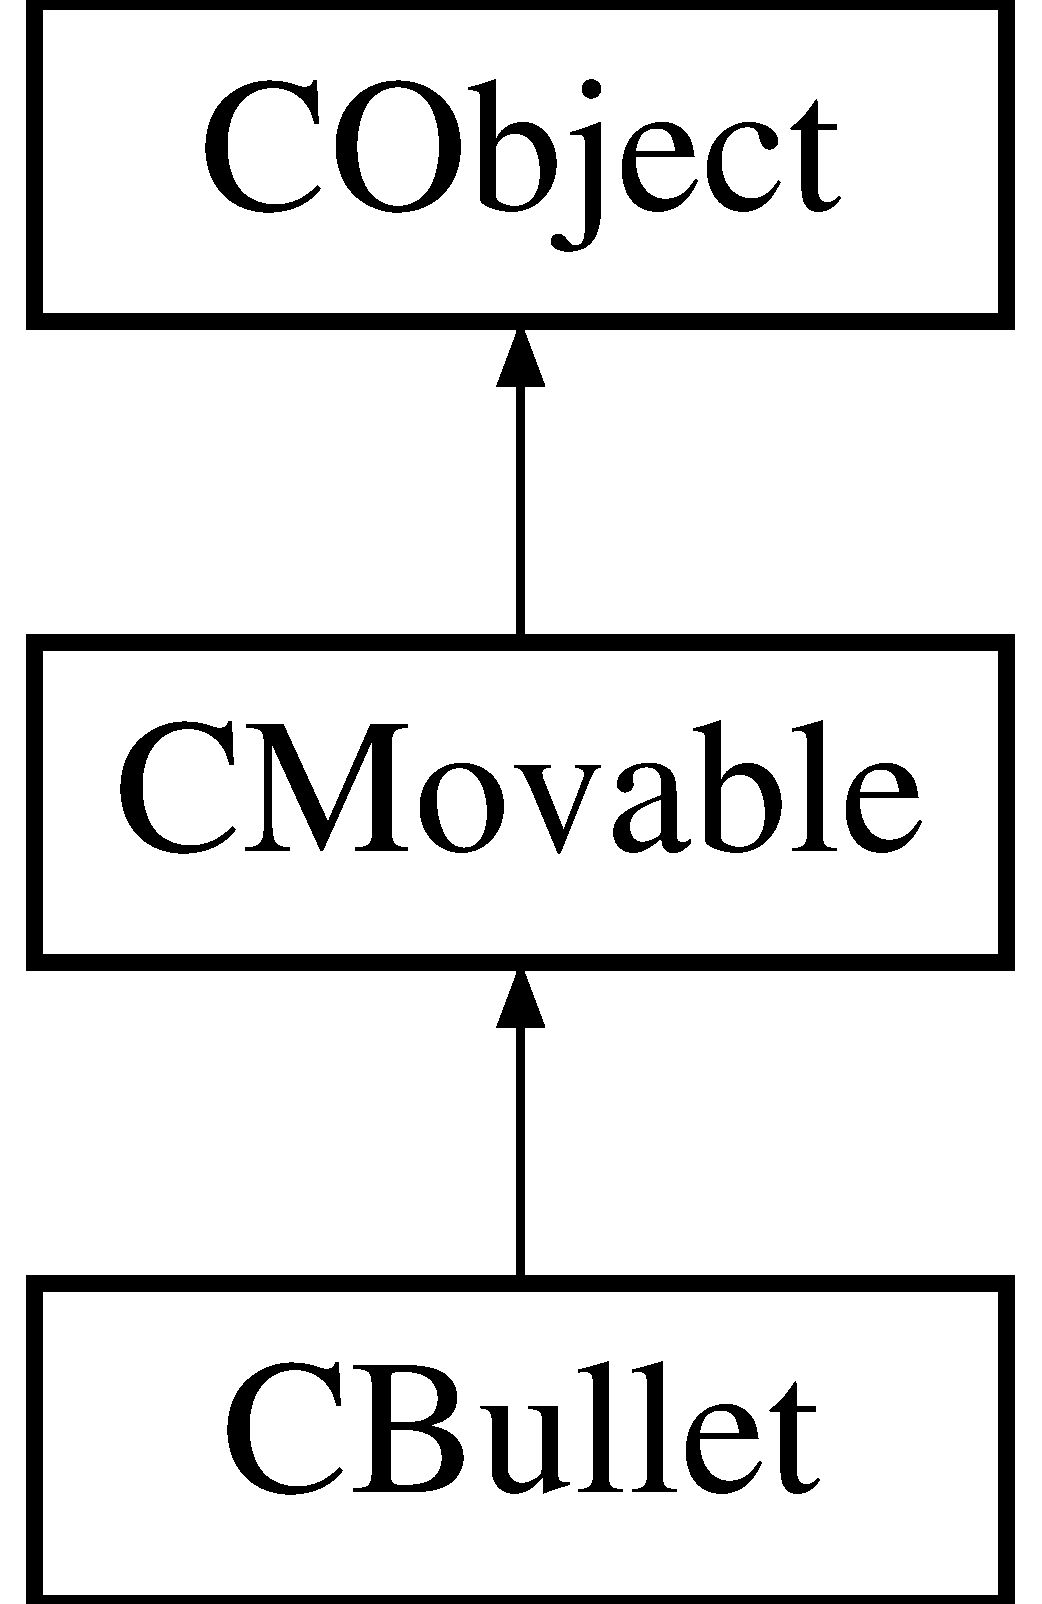
\includegraphics[height=3.000000cm]{class_c_bullet}
\end{center}
\end{figure}
\subsection*{Public Member Functions}
\begin{DoxyCompactItemize}
\item 
\mbox{\hyperlink{class_c_bullet_a56797cd539f173bbfc8cc9d238734fbc}{C\+Bullet}} (\mbox{\hyperlink{class_c_map}{C\+Map}} $\ast$m, \mbox{\hyperlink{class_c_fighting_robot}{C\+Fighting\+Robot}} $\ast$r)
\begin{DoxyCompactList}\small\item\em Poza dodatkowym wskaźnikiem do robota, konstruktor analogiczny do reszty ruchomych obiektów. \end{DoxyCompactList}\item 
virtual \mbox{\hyperlink{class_c_bullet_ac3502e35a7797b9d7d0efef288618a71}{$\sim$\+C\+Bullet}} ()
\item 
void \mbox{\hyperlink{class_c_bullet_a693e95f219a9a642e3977bb48be0cf5d}{move}} ()
\begin{DoxyCompactList}\small\item\em Przy każdym wywołaniu przesuwa obiekt ze stałą prędkością w kierunku, w którym został wystrzelony. \end{DoxyCompactList}\item 
void \mbox{\hyperlink{class_c_bullet_a9685917f7fc76d417e03744223b1b2c6}{update}} ()
\begin{DoxyCompactList}\small\item\em Przy każdym wywołaniu sprawdza otoczenie; jeśli koliduje z jakimś robotem, który go nie wystrzelił, usuwa tego robota; jeśli życie pocisku jest równe zero, usuwa pocisk; jeśli nie, wywołuje \mbox{\hyperlink{class_c_bullet_a693e95f219a9a642e3977bb48be0cf5d}{move()}} i dekrementuje życie pocisku oraz zmniejsza jego rozmiar. \end{DoxyCompactList}\end{DoxyCompactItemize}
\subsection*{Additional Inherited Members}


\subsection{Detailed Description}
Pociski wystrzeliwywane przez roboty walczące. 

\subsection{Constructor \& Destructor Documentation}
\mbox{\Hypertarget{class_c_bullet_a56797cd539f173bbfc8cc9d238734fbc}\label{class_c_bullet_a56797cd539f173bbfc8cc9d238734fbc}} 
\index{C\+Bullet@{C\+Bullet}!C\+Bullet@{C\+Bullet}}
\index{C\+Bullet@{C\+Bullet}!C\+Bullet@{C\+Bullet}}
\subsubsection{\texorpdfstring{C\+Bullet()}{CBullet()}}
{\footnotesize\ttfamily C\+Bullet\+::\+C\+Bullet (\begin{DoxyParamCaption}\item[{\mbox{\hyperlink{class_c_map}{C\+Map}} $\ast$}]{m,  }\item[{\mbox{\hyperlink{class_c_fighting_robot}{C\+Fighting\+Robot}} $\ast$}]{r }\end{DoxyParamCaption})}



Poza dodatkowym wskaźnikiem do robota, konstruktor analogiczny do reszty ruchomych obiektów. 


\begin{DoxyParams}{Parameters}
{\em r} & wskaźnik na robota, który wystrzelił dany pocisk \\
\hline
\end{DoxyParams}
\mbox{\Hypertarget{class_c_bullet_ac3502e35a7797b9d7d0efef288618a71}\label{class_c_bullet_ac3502e35a7797b9d7d0efef288618a71}} 
\index{C\+Bullet@{C\+Bullet}!````~C\+Bullet@{$\sim$\+C\+Bullet}}
\index{````~C\+Bullet@{$\sim$\+C\+Bullet}!C\+Bullet@{C\+Bullet}}
\subsubsection{\texorpdfstring{$\sim$\+C\+Bullet()}{~CBullet()}}
{\footnotesize\ttfamily C\+Bullet\+::$\sim$\+C\+Bullet (\begin{DoxyParamCaption}{ }\end{DoxyParamCaption})\hspace{0.3cm}{\ttfamily [virtual]}}



\subsection{Member Function Documentation}
\mbox{\Hypertarget{class_c_bullet_a693e95f219a9a642e3977bb48be0cf5d}\label{class_c_bullet_a693e95f219a9a642e3977bb48be0cf5d}} 
\index{C\+Bullet@{C\+Bullet}!move@{move}}
\index{move@{move}!C\+Bullet@{C\+Bullet}}
\subsubsection{\texorpdfstring{move()}{move()}}
{\footnotesize\ttfamily void C\+Bullet\+::move (\begin{DoxyParamCaption}{ }\end{DoxyParamCaption})\hspace{0.3cm}{\ttfamily [virtual]}}



Przy każdym wywołaniu przesuwa obiekt ze stałą prędkością w kierunku, w którym został wystrzelony. 



Implements \mbox{\hyperlink{class_c_movable_a8e66e106f13362d24462ce0c9d0431af}{C\+Movable}}.

\mbox{\Hypertarget{class_c_bullet_a9685917f7fc76d417e03744223b1b2c6}\label{class_c_bullet_a9685917f7fc76d417e03744223b1b2c6}} 
\index{C\+Bullet@{C\+Bullet}!update@{update}}
\index{update@{update}!C\+Bullet@{C\+Bullet}}
\subsubsection{\texorpdfstring{update()}{update()}}
{\footnotesize\ttfamily void C\+Bullet\+::update (\begin{DoxyParamCaption}{ }\end{DoxyParamCaption})\hspace{0.3cm}{\ttfamily [virtual]}}



Przy każdym wywołaniu sprawdza otoczenie; jeśli koliduje z jakimś robotem, który go nie wystrzelił, usuwa tego robota; jeśli życie pocisku jest równe zero, usuwa pocisk; jeśli nie, wywołuje \mbox{\hyperlink{class_c_bullet_a693e95f219a9a642e3977bb48be0cf5d}{move()}} i dekrementuje życie pocisku oraz zmniejsza jego rozmiar. 



Implements \mbox{\hyperlink{class_c_movable_af45fc62960d86ef62949d078141e9d62}{C\+Movable}}.



The documentation for this class was generated from the following files\+:\begin{DoxyCompactItemize}
\item 
\mbox{\hyperlink{cbullet_8h}{cbullet.\+h}}\item 
\mbox{\hyperlink{cbullet_8cpp}{cbullet.\+cpp}}\end{DoxyCompactItemize}

\hypertarget{class_c_cleaning_robot}{}\section{C\+Cleaning\+Robot Class Reference}
\label{class_c_cleaning_robot}\index{C\+Cleaning\+Robot@{C\+Cleaning\+Robot}}


Robot zajmujący się sprzątaniem brudów z mapy.  




{\ttfamily \#include $<$ccleaningrobot.\+h$>$}

Inheritance diagram for C\+Cleaning\+Robot\+:\begin{figure}[H]
\begin{center}
\leavevmode
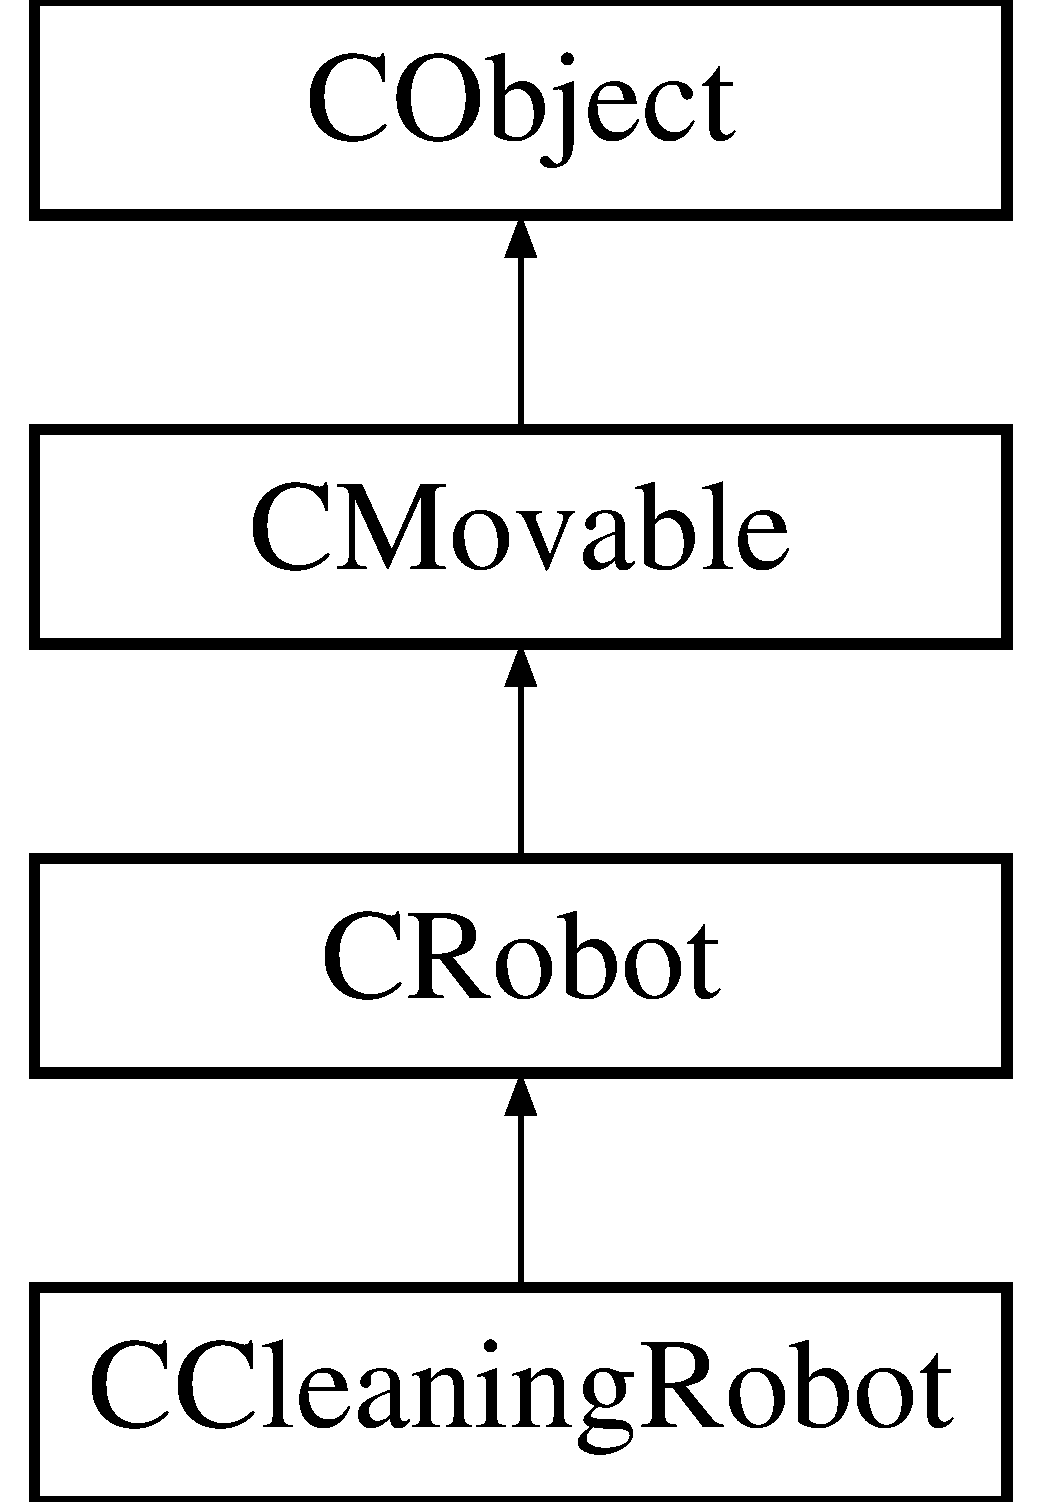
\includegraphics[height=4.000000cm]{class_c_cleaning_robot}
\end{center}
\end{figure}
\subsection*{Public Member Functions}
\begin{DoxyCompactItemize}
\item 
\mbox{\hyperlink{class_c_cleaning_robot_a0d304b4d201832056a946d6ee0a1141c}{C\+Cleaning\+Robot}} (\mbox{\hyperlink{class_c_map}{C\+Map}} $\ast$m)
\item 
\mbox{\hyperlink{class_c_cleaning_robot_ae22783fb4dd66322b3d63e2ac6beb4a6}{C\+Cleaning\+Robot}} (qreal xv, qreal yv, \mbox{\hyperlink{class_c_map}{C\+Map}} $\ast$m)
\item 
\mbox{\hyperlink{class_c_cleaning_robot_af00faa2e7ae3c1b62a026abe39df0a44}{C\+Cleaning\+Robot}} (qreal xv, qreal yv, qreal anglev, qreal rangev, \mbox{\hyperlink{class_c_map}{C\+Map}} $\ast$m)
\item 
virtual \mbox{\hyperlink{class_c_cleaning_robot_a8622a44357356261e13c30de8915381b}{$\sim$\+C\+Cleaning\+Robot}} ()
\item 
void \mbox{\hyperlink{class_c_cleaning_robot_a1ad227a5f3508a8e78fcecae7d3de53b}{move}} ()
\begin{DoxyCompactList}\small\item\em Funkcja stara się w pierwszej kolejności uniknąć kolizji z innymi obiektami; jeśli nie wystąpi kolizja, sprawdzane jest, czy robot jest na mapie; jeśli nie jest na mapie, próbuje wrócić i kończy ruch; w przeciwnym wypadku kieruje się w stronę najbliższego brudu, o ile jakieś są w zasięgu; jeśli w pobliżu nie ma żadnych brudów, robot porusza się losowo. \end{DoxyCompactList}\item 
void \mbox{\hyperlink{class_c_cleaning_robot_afd8b3a58abfc91ebdce32af3686c5e9f}{update}} ()
\begin{DoxyCompactList}\small\item\em Funkcja sprawdza, czy występują kolizje z jakimiś brudami i usuwa ewentualne kolidujące brudy; następnie wywoływana jest funkcja \mbox{\hyperlink{class_c_cleaning_robot_a1ad227a5f3508a8e78fcecae7d3de53b}{move()}} \end{DoxyCompactList}\item 
void \mbox{\hyperlink{class_c_cleaning_robot_a1c106e1736653d8c0f24fbb9f1820f79}{clean}} (\mbox{\hyperlink{class_c_dirt}{C\+Dirt}} $\ast$dirt)
\begin{DoxyCompactList}\small\item\em Funkcja usuwa podany obiekt. \end{DoxyCompactList}\end{DoxyCompactItemize}
\subsection*{Additional Inherited Members}


\subsection{Detailed Description}
Robot zajmujący się sprzątaniem brudów z mapy. 

\subsection{Constructor \& Destructor Documentation}
\mbox{\Hypertarget{class_c_cleaning_robot_a0d304b4d201832056a946d6ee0a1141c}\label{class_c_cleaning_robot_a0d304b4d201832056a946d6ee0a1141c}} 
\index{C\+Cleaning\+Robot@{C\+Cleaning\+Robot}!C\+Cleaning\+Robot@{C\+Cleaning\+Robot}}
\index{C\+Cleaning\+Robot@{C\+Cleaning\+Robot}!C\+Cleaning\+Robot@{C\+Cleaning\+Robot}}
\subsubsection{\texorpdfstring{C\+Cleaning\+Robot()}{CCleaningRobot()}\hspace{0.1cm}{\footnotesize\ttfamily [1/3]}}
{\footnotesize\ttfamily C\+Cleaning\+Robot\+::\+C\+Cleaning\+Robot (\begin{DoxyParamCaption}\item[{\mbox{\hyperlink{class_c_map}{C\+Map}} $\ast$}]{m }\end{DoxyParamCaption})}

\mbox{\Hypertarget{class_c_cleaning_robot_ae22783fb4dd66322b3d63e2ac6beb4a6}\label{class_c_cleaning_robot_ae22783fb4dd66322b3d63e2ac6beb4a6}} 
\index{C\+Cleaning\+Robot@{C\+Cleaning\+Robot}!C\+Cleaning\+Robot@{C\+Cleaning\+Robot}}
\index{C\+Cleaning\+Robot@{C\+Cleaning\+Robot}!C\+Cleaning\+Robot@{C\+Cleaning\+Robot}}
\subsubsection{\texorpdfstring{C\+Cleaning\+Robot()}{CCleaningRobot()}\hspace{0.1cm}{\footnotesize\ttfamily [2/3]}}
{\footnotesize\ttfamily C\+Cleaning\+Robot\+::\+C\+Cleaning\+Robot (\begin{DoxyParamCaption}\item[{qreal}]{xv,  }\item[{qreal}]{yv,  }\item[{\mbox{\hyperlink{class_c_map}{C\+Map}} $\ast$}]{m }\end{DoxyParamCaption})}

\mbox{\Hypertarget{class_c_cleaning_robot_af00faa2e7ae3c1b62a026abe39df0a44}\label{class_c_cleaning_robot_af00faa2e7ae3c1b62a026abe39df0a44}} 
\index{C\+Cleaning\+Robot@{C\+Cleaning\+Robot}!C\+Cleaning\+Robot@{C\+Cleaning\+Robot}}
\index{C\+Cleaning\+Robot@{C\+Cleaning\+Robot}!C\+Cleaning\+Robot@{C\+Cleaning\+Robot}}
\subsubsection{\texorpdfstring{C\+Cleaning\+Robot()}{CCleaningRobot()}\hspace{0.1cm}{\footnotesize\ttfamily [3/3]}}
{\footnotesize\ttfamily C\+Cleaning\+Robot\+::\+C\+Cleaning\+Robot (\begin{DoxyParamCaption}\item[{qreal}]{xv,  }\item[{qreal}]{yv,  }\item[{qreal}]{anglev,  }\item[{qreal}]{rangev,  }\item[{\mbox{\hyperlink{class_c_map}{C\+Map}} $\ast$}]{m }\end{DoxyParamCaption})}

\mbox{\Hypertarget{class_c_cleaning_robot_a8622a44357356261e13c30de8915381b}\label{class_c_cleaning_robot_a8622a44357356261e13c30de8915381b}} 
\index{C\+Cleaning\+Robot@{C\+Cleaning\+Robot}!````~C\+Cleaning\+Robot@{$\sim$\+C\+Cleaning\+Robot}}
\index{````~C\+Cleaning\+Robot@{$\sim$\+C\+Cleaning\+Robot}!C\+Cleaning\+Robot@{C\+Cleaning\+Robot}}
\subsubsection{\texorpdfstring{$\sim$\+C\+Cleaning\+Robot()}{~CCleaningRobot()}}
{\footnotesize\ttfamily C\+Cleaning\+Robot\+::$\sim$\+C\+Cleaning\+Robot (\begin{DoxyParamCaption}{ }\end{DoxyParamCaption})\hspace{0.3cm}{\ttfamily [virtual]}}



\subsection{Member Function Documentation}
\mbox{\Hypertarget{class_c_cleaning_robot_a1c106e1736653d8c0f24fbb9f1820f79}\label{class_c_cleaning_robot_a1c106e1736653d8c0f24fbb9f1820f79}} 
\index{C\+Cleaning\+Robot@{C\+Cleaning\+Robot}!clean@{clean}}
\index{clean@{clean}!C\+Cleaning\+Robot@{C\+Cleaning\+Robot}}
\subsubsection{\texorpdfstring{clean()}{clean()}}
{\footnotesize\ttfamily void C\+Cleaning\+Robot\+::clean (\begin{DoxyParamCaption}\item[{\mbox{\hyperlink{class_c_dirt}{C\+Dirt}} $\ast$}]{dirt }\end{DoxyParamCaption})}



Funkcja usuwa podany obiekt. 


\begin{DoxyParams}{Parameters}
{\em dirt} & Brud, który chcemy usunąć \\
\hline
\end{DoxyParams}
\mbox{\Hypertarget{class_c_cleaning_robot_a1ad227a5f3508a8e78fcecae7d3de53b}\label{class_c_cleaning_robot_a1ad227a5f3508a8e78fcecae7d3de53b}} 
\index{C\+Cleaning\+Robot@{C\+Cleaning\+Robot}!move@{move}}
\index{move@{move}!C\+Cleaning\+Robot@{C\+Cleaning\+Robot}}
\subsubsection{\texorpdfstring{move()}{move()}}
{\footnotesize\ttfamily void C\+Cleaning\+Robot\+::move (\begin{DoxyParamCaption}{ }\end{DoxyParamCaption})\hspace{0.3cm}{\ttfamily [virtual]}}



Funkcja stara się w pierwszej kolejności uniknąć kolizji z innymi obiektami; jeśli nie wystąpi kolizja, sprawdzane jest, czy robot jest na mapie; jeśli nie jest na mapie, próbuje wrócić i kończy ruch; w przeciwnym wypadku kieruje się w stronę najbliższego brudu, o ile jakieś są w zasięgu; jeśli w pobliżu nie ma żadnych brudów, robot porusza się losowo. 



Implements \mbox{\hyperlink{class_c_robot_a1de9be879213eadf7ded27caedb84598}{C\+Robot}}.

\mbox{\Hypertarget{class_c_cleaning_robot_afd8b3a58abfc91ebdce32af3686c5e9f}\label{class_c_cleaning_robot_afd8b3a58abfc91ebdce32af3686c5e9f}} 
\index{C\+Cleaning\+Robot@{C\+Cleaning\+Robot}!update@{update}}
\index{update@{update}!C\+Cleaning\+Robot@{C\+Cleaning\+Robot}}
\subsubsection{\texorpdfstring{update()}{update()}}
{\footnotesize\ttfamily void C\+Cleaning\+Robot\+::update (\begin{DoxyParamCaption}{ }\end{DoxyParamCaption})\hspace{0.3cm}{\ttfamily [virtual]}}



Funkcja sprawdza, czy występują kolizje z jakimiś brudami i usuwa ewentualne kolidujące brudy; następnie wywoływana jest funkcja \mbox{\hyperlink{class_c_cleaning_robot_a1ad227a5f3508a8e78fcecae7d3de53b}{move()}} 



Implements \mbox{\hyperlink{class_c_robot_a8ad8d55a840ced20f85a2a045e9e24ef}{C\+Robot}}.



The documentation for this class was generated from the following files\+:\begin{DoxyCompactItemize}
\item 
\mbox{\hyperlink{ccleaningrobot_8h}{ccleaningrobot.\+h}}\item 
\mbox{\hyperlink{ccleaningrobot_8cpp}{ccleaningrobot.\+cpp}}\end{DoxyCompactItemize}

\hypertarget{class_c_dirt}{}\section{C\+Dirt Class Reference}
\label{class_c_dirt}\index{C\+Dirt@{C\+Dirt}}


Brudy zbierane przez roboty sprzątające.  




{\ttfamily \#include $<$cdirt.\+h$>$}

Inheritance diagram for C\+Dirt\+:\begin{figure}[H]
\begin{center}
\leavevmode
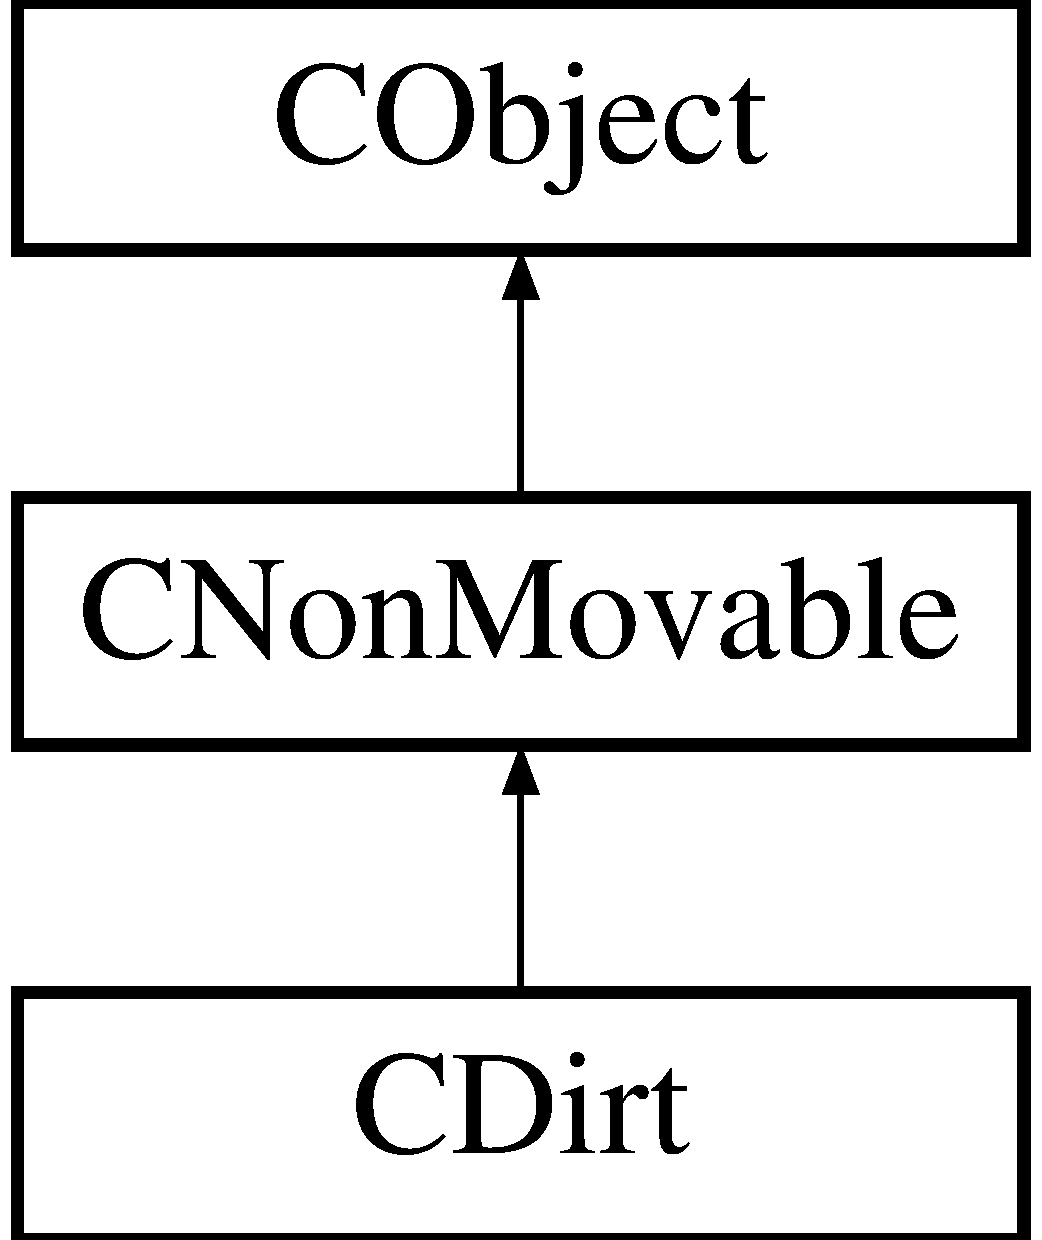
\includegraphics[height=3.000000cm]{class_c_dirt}
\end{center}
\end{figure}
\subsection*{Public Member Functions}
\begin{DoxyCompactItemize}
\item 
\mbox{\hyperlink{class_c_dirt_ac6f6303193035707f229f8569edfdcfc}{C\+Dirt}} (\mbox{\hyperlink{class_c_map}{C\+Map}} $\ast$m)
\item 
virtual \mbox{\hyperlink{class_c_dirt_a1cd1a70d7c690518f7dbd1a93e6d3da4}{$\sim$\+C\+Dirt}} ()
\item 
void \mbox{\hyperlink{class_c_dirt_a0f077e7fde1b397f08659f65d28cf573}{update}} ()
\begin{DoxyCompactList}\small\item\em W każdej turze losowo może nastąpić rozrost brudu. \end{DoxyCompactList}\item 
void \mbox{\hyperlink{class_c_dirt_a20be69acaff474646f86b128c0fd65f0}{get\+Cleaned}} ()
\begin{DoxyCompactList}\small\item\em Funkcja wywoływana w celu usunięcia danego brudu. \end{DoxyCompactList}\end{DoxyCompactItemize}
\subsection*{Additional Inherited Members}


\subsection{Detailed Description}
Brudy zbierane przez roboty sprzątające. 

\subsection{Constructor \& Destructor Documentation}
\mbox{\Hypertarget{class_c_dirt_ac6f6303193035707f229f8569edfdcfc}\label{class_c_dirt_ac6f6303193035707f229f8569edfdcfc}} 
\index{C\+Dirt@{C\+Dirt}!C\+Dirt@{C\+Dirt}}
\index{C\+Dirt@{C\+Dirt}!C\+Dirt@{C\+Dirt}}
\subsubsection{\texorpdfstring{C\+Dirt()}{CDirt()}}
{\footnotesize\ttfamily C\+Dirt\+::\+C\+Dirt (\begin{DoxyParamCaption}\item[{\mbox{\hyperlink{class_c_map}{C\+Map}} $\ast$}]{m }\end{DoxyParamCaption})}

\mbox{\Hypertarget{class_c_dirt_a1cd1a70d7c690518f7dbd1a93e6d3da4}\label{class_c_dirt_a1cd1a70d7c690518f7dbd1a93e6d3da4}} 
\index{C\+Dirt@{C\+Dirt}!````~C\+Dirt@{$\sim$\+C\+Dirt}}
\index{````~C\+Dirt@{$\sim$\+C\+Dirt}!C\+Dirt@{C\+Dirt}}
\subsubsection{\texorpdfstring{$\sim$\+C\+Dirt()}{~CDirt()}}
{\footnotesize\ttfamily C\+Dirt\+::$\sim$\+C\+Dirt (\begin{DoxyParamCaption}{ }\end{DoxyParamCaption})\hspace{0.3cm}{\ttfamily [virtual]}}



\subsection{Member Function Documentation}
\mbox{\Hypertarget{class_c_dirt_a20be69acaff474646f86b128c0fd65f0}\label{class_c_dirt_a20be69acaff474646f86b128c0fd65f0}} 
\index{C\+Dirt@{C\+Dirt}!get\+Cleaned@{get\+Cleaned}}
\index{get\+Cleaned@{get\+Cleaned}!C\+Dirt@{C\+Dirt}}
\subsubsection{\texorpdfstring{get\+Cleaned()}{getCleaned()}}
{\footnotesize\ttfamily void C\+Dirt\+::get\+Cleaned (\begin{DoxyParamCaption}{ }\end{DoxyParamCaption})}



Funkcja wywoływana w celu usunięcia danego brudu. 

\mbox{\Hypertarget{class_c_dirt_a0f077e7fde1b397f08659f65d28cf573}\label{class_c_dirt_a0f077e7fde1b397f08659f65d28cf573}} 
\index{C\+Dirt@{C\+Dirt}!update@{update}}
\index{update@{update}!C\+Dirt@{C\+Dirt}}
\subsubsection{\texorpdfstring{update()}{update()}}
{\footnotesize\ttfamily void C\+Dirt\+::update (\begin{DoxyParamCaption}{ }\end{DoxyParamCaption})\hspace{0.3cm}{\ttfamily [virtual]}}



W każdej turze losowo może nastąpić rozrost brudu. 



Implements \mbox{\hyperlink{class_c_non_movable_ace03bea0246940c6c5c0b26ffa1ef165}{C\+Non\+Movable}}.



The documentation for this class was generated from the following files\+:\begin{DoxyCompactItemize}
\item 
\mbox{\hyperlink{cdirt_8h}{cdirt.\+h}}\item 
\mbox{\hyperlink{cdirt_8cpp}{cdirt.\+cpp}}\end{DoxyCompactItemize}

\hypertarget{class_c_fighting_robot}{}\section{C\+Fighting\+Robot Class Reference}
\label{class_c_fighting_robot}\index{C\+Fighting\+Robot@{C\+Fighting\+Robot}}


Robot atakujący inne roboty.  




{\ttfamily \#include $<$cfightingrobot.\+h$>$}

Inheritance diagram for C\+Fighting\+Robot\+:\begin{figure}[H]
\begin{center}
\leavevmode
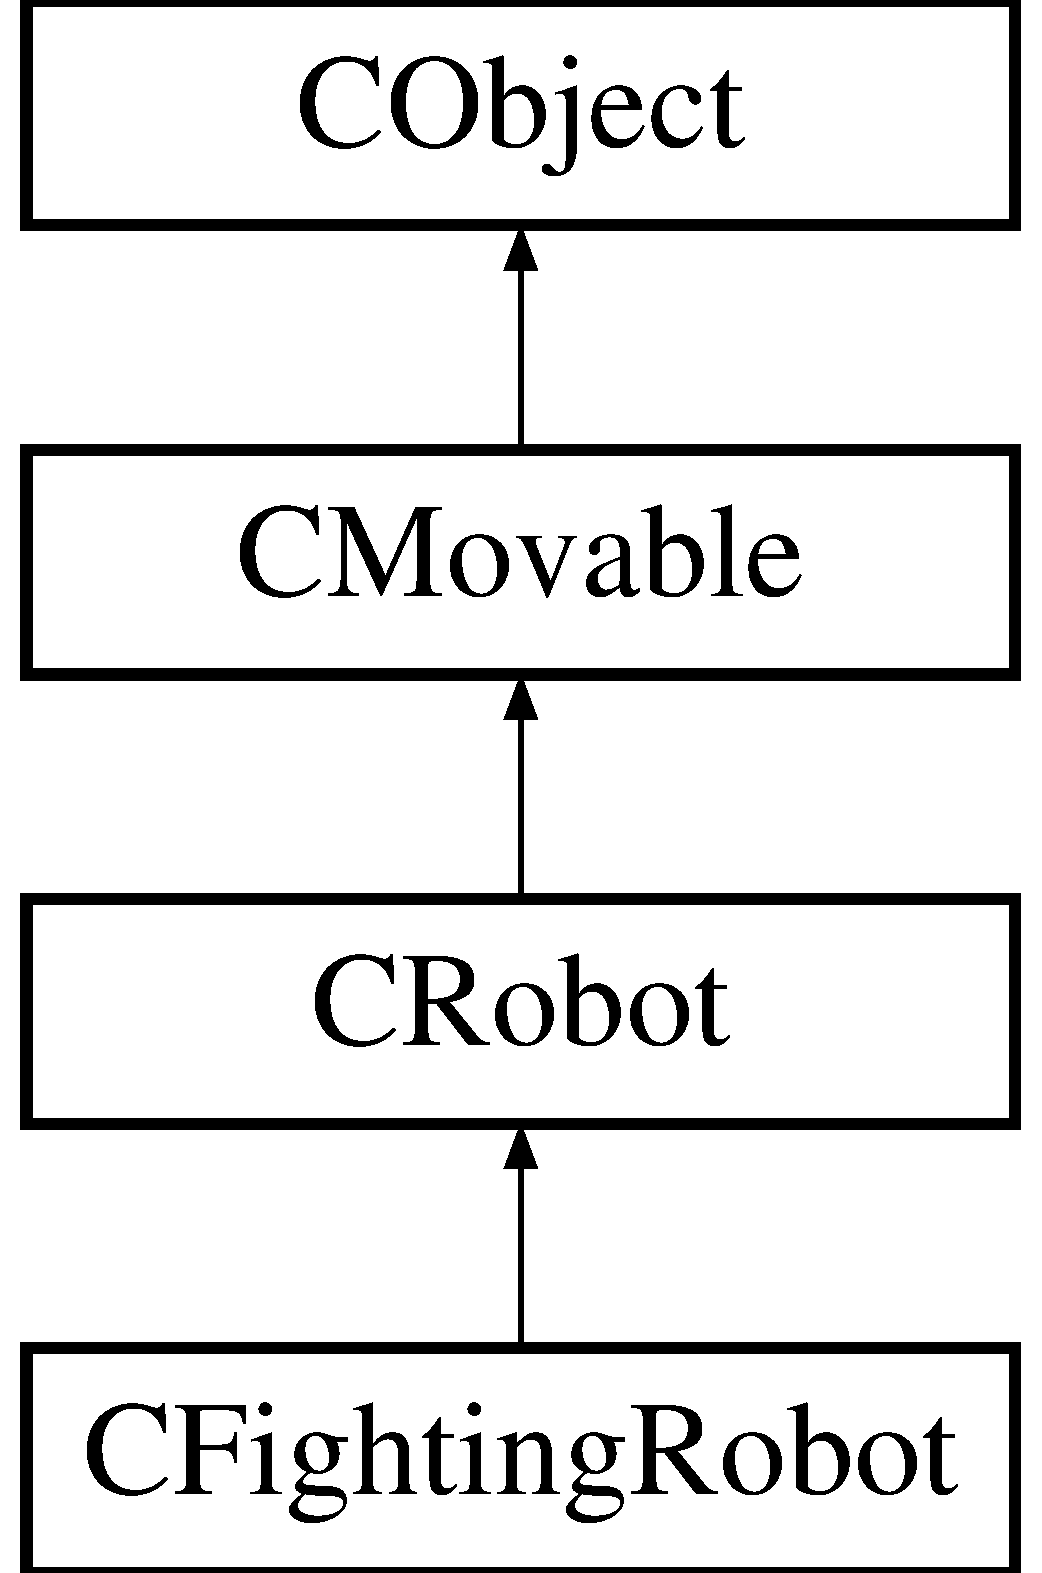
\includegraphics[height=4.000000cm]{class_c_fighting_robot}
\end{center}
\end{figure}
\subsection*{Public Member Functions}
\begin{DoxyCompactItemize}
\item 
\mbox{\hyperlink{class_c_fighting_robot_a0930ab24dba8a1c3b6f7a6cb693d59bf}{C\+Fighting\+Robot}} (\mbox{\hyperlink{class_c_map}{C\+Map}} $\ast$m)
\item 
\mbox{\hyperlink{class_c_fighting_robot_a65deb458a3628c7c5e7898928e3a077c}{C\+Fighting\+Robot}} (qreal xv, qreal yv, \mbox{\hyperlink{class_c_map}{C\+Map}} $\ast$m)
\item 
\mbox{\hyperlink{class_c_fighting_robot_ab9f9806093c0def1cde010de151c55e5}{C\+Fighting\+Robot}} (qreal xv, qreal yv, qreal anglev, qreal rangev, \mbox{\hyperlink{class_c_map}{C\+Map}} $\ast$m)
\item 
virtual \mbox{\hyperlink{class_c_fighting_robot_aa47308cfbd10635eedebe8063d478a72}{$\sim$\+C\+Fighting\+Robot}} ()
\item 
void \mbox{\hyperlink{class_c_fighting_robot_af644acbba178e256566e9dbd230aa4db}{move}} ()
\begin{DoxyCompactList}\small\item\em Funkcja stara się w pierwszej kolejności uniknąć kolizji z innymi obiektami; jeśli nie wystąpi kolizja, sprawdzane jest, czy robot jest na mapie; jeśli nie jest na mapie, próbuje wrócić i kończy ruch; w przeciwnym wypadku kieruje się w stronę najbliższego robota, o ile jakieś są w zasięgu; jeśli w pobliżu nie ma żadnych brudów, robot porusza się losowo. \end{DoxyCompactList}\item 
void \mbox{\hyperlink{class_c_fighting_robot_a3ae0ea383f809766e53c81348a07daaa}{update}} ()
\begin{DoxyCompactList}\small\item\em Funkcja sprawdza, czy w pobliżu są jakieś roboty, które można zaatakować i wywołuje funkcję \mbox{\hyperlink{class_c_fighting_robot_a6a97cdc69ce705f810d657a31a3afbbd}{attack()}} na ewentualnych robotach; następnie wywoływana jest funkcja \mbox{\hyperlink{class_c_fighting_robot_af644acbba178e256566e9dbd230aa4db}{move()}} \end{DoxyCompactList}\item 
void \mbox{\hyperlink{class_c_fighting_robot_a6a97cdc69ce705f810d657a31a3afbbd}{attack}} (\mbox{\hyperlink{class_c_robot}{C\+Robot}} $\ast$robot)
\begin{DoxyCompactList}\small\item\em Tworzy pocisk i wysyła go w kierunku podanego robota. \end{DoxyCompactList}\end{DoxyCompactItemize}
\subsection*{Additional Inherited Members}


\subsection{Detailed Description}
Robot atakujący inne roboty. 

\subsection{Constructor \& Destructor Documentation}
\mbox{\Hypertarget{class_c_fighting_robot_a0930ab24dba8a1c3b6f7a6cb693d59bf}\label{class_c_fighting_robot_a0930ab24dba8a1c3b6f7a6cb693d59bf}} 
\index{C\+Fighting\+Robot@{C\+Fighting\+Robot}!C\+Fighting\+Robot@{C\+Fighting\+Robot}}
\index{C\+Fighting\+Robot@{C\+Fighting\+Robot}!C\+Fighting\+Robot@{C\+Fighting\+Robot}}
\subsubsection{\texorpdfstring{C\+Fighting\+Robot()}{CFightingRobot()}\hspace{0.1cm}{\footnotesize\ttfamily [1/3]}}
{\footnotesize\ttfamily C\+Fighting\+Robot\+::\+C\+Fighting\+Robot (\begin{DoxyParamCaption}\item[{\mbox{\hyperlink{class_c_map}{C\+Map}} $\ast$}]{m }\end{DoxyParamCaption})}

\mbox{\Hypertarget{class_c_fighting_robot_a65deb458a3628c7c5e7898928e3a077c}\label{class_c_fighting_robot_a65deb458a3628c7c5e7898928e3a077c}} 
\index{C\+Fighting\+Robot@{C\+Fighting\+Robot}!C\+Fighting\+Robot@{C\+Fighting\+Robot}}
\index{C\+Fighting\+Robot@{C\+Fighting\+Robot}!C\+Fighting\+Robot@{C\+Fighting\+Robot}}
\subsubsection{\texorpdfstring{C\+Fighting\+Robot()}{CFightingRobot()}\hspace{0.1cm}{\footnotesize\ttfamily [2/3]}}
{\footnotesize\ttfamily C\+Fighting\+Robot\+::\+C\+Fighting\+Robot (\begin{DoxyParamCaption}\item[{qreal}]{xv,  }\item[{qreal}]{yv,  }\item[{\mbox{\hyperlink{class_c_map}{C\+Map}} $\ast$}]{m }\end{DoxyParamCaption})}

\mbox{\Hypertarget{class_c_fighting_robot_ab9f9806093c0def1cde010de151c55e5}\label{class_c_fighting_robot_ab9f9806093c0def1cde010de151c55e5}} 
\index{C\+Fighting\+Robot@{C\+Fighting\+Robot}!C\+Fighting\+Robot@{C\+Fighting\+Robot}}
\index{C\+Fighting\+Robot@{C\+Fighting\+Robot}!C\+Fighting\+Robot@{C\+Fighting\+Robot}}
\subsubsection{\texorpdfstring{C\+Fighting\+Robot()}{CFightingRobot()}\hspace{0.1cm}{\footnotesize\ttfamily [3/3]}}
{\footnotesize\ttfamily C\+Fighting\+Robot\+::\+C\+Fighting\+Robot (\begin{DoxyParamCaption}\item[{qreal}]{xv,  }\item[{qreal}]{yv,  }\item[{qreal}]{anglev,  }\item[{qreal}]{rangev,  }\item[{\mbox{\hyperlink{class_c_map}{C\+Map}} $\ast$}]{m }\end{DoxyParamCaption})}

\mbox{\Hypertarget{class_c_fighting_robot_aa47308cfbd10635eedebe8063d478a72}\label{class_c_fighting_robot_aa47308cfbd10635eedebe8063d478a72}} 
\index{C\+Fighting\+Robot@{C\+Fighting\+Robot}!````~C\+Fighting\+Robot@{$\sim$\+C\+Fighting\+Robot}}
\index{````~C\+Fighting\+Robot@{$\sim$\+C\+Fighting\+Robot}!C\+Fighting\+Robot@{C\+Fighting\+Robot}}
\subsubsection{\texorpdfstring{$\sim$\+C\+Fighting\+Robot()}{~CFightingRobot()}}
{\footnotesize\ttfamily C\+Fighting\+Robot\+::$\sim$\+C\+Fighting\+Robot (\begin{DoxyParamCaption}{ }\end{DoxyParamCaption})\hspace{0.3cm}{\ttfamily [virtual]}}



\subsection{Member Function Documentation}
\mbox{\Hypertarget{class_c_fighting_robot_a6a97cdc69ce705f810d657a31a3afbbd}\label{class_c_fighting_robot_a6a97cdc69ce705f810d657a31a3afbbd}} 
\index{C\+Fighting\+Robot@{C\+Fighting\+Robot}!attack@{attack}}
\index{attack@{attack}!C\+Fighting\+Robot@{C\+Fighting\+Robot}}
\subsubsection{\texorpdfstring{attack()}{attack()}}
{\footnotesize\ttfamily void C\+Fighting\+Robot\+::attack (\begin{DoxyParamCaption}\item[{\mbox{\hyperlink{class_c_robot}{C\+Robot}} $\ast$}]{robot }\end{DoxyParamCaption})}



Tworzy pocisk i wysyła go w kierunku podanego robota. 


\begin{DoxyParams}{Parameters}
{\em robot} & Robot, którego należy zaatakować \\
\hline
\end{DoxyParams}
\mbox{\Hypertarget{class_c_fighting_robot_af644acbba178e256566e9dbd230aa4db}\label{class_c_fighting_robot_af644acbba178e256566e9dbd230aa4db}} 
\index{C\+Fighting\+Robot@{C\+Fighting\+Robot}!move@{move}}
\index{move@{move}!C\+Fighting\+Robot@{C\+Fighting\+Robot}}
\subsubsection{\texorpdfstring{move()}{move()}}
{\footnotesize\ttfamily void C\+Fighting\+Robot\+::move (\begin{DoxyParamCaption}{ }\end{DoxyParamCaption})\hspace{0.3cm}{\ttfamily [virtual]}}



Funkcja stara się w pierwszej kolejności uniknąć kolizji z innymi obiektami; jeśli nie wystąpi kolizja, sprawdzane jest, czy robot jest na mapie; jeśli nie jest na mapie, próbuje wrócić i kończy ruch; w przeciwnym wypadku kieruje się w stronę najbliższego robota, o ile jakieś są w zasięgu; jeśli w pobliżu nie ma żadnych brudów, robot porusza się losowo. 



Implements \mbox{\hyperlink{class_c_robot_a1de9be879213eadf7ded27caedb84598}{C\+Robot}}.

\mbox{\Hypertarget{class_c_fighting_robot_a3ae0ea383f809766e53c81348a07daaa}\label{class_c_fighting_robot_a3ae0ea383f809766e53c81348a07daaa}} 
\index{C\+Fighting\+Robot@{C\+Fighting\+Robot}!update@{update}}
\index{update@{update}!C\+Fighting\+Robot@{C\+Fighting\+Robot}}
\subsubsection{\texorpdfstring{update()}{update()}}
{\footnotesize\ttfamily void C\+Fighting\+Robot\+::update (\begin{DoxyParamCaption}{ }\end{DoxyParamCaption})\hspace{0.3cm}{\ttfamily [virtual]}}



Funkcja sprawdza, czy w pobliżu są jakieś roboty, które można zaatakować i wywołuje funkcję \mbox{\hyperlink{class_c_fighting_robot_a6a97cdc69ce705f810d657a31a3afbbd}{attack()}} na ewentualnych robotach; następnie wywoływana jest funkcja \mbox{\hyperlink{class_c_fighting_robot_af644acbba178e256566e9dbd230aa4db}{move()}} 



Implements \mbox{\hyperlink{class_c_robot_a8ad8d55a840ced20f85a2a045e9e24ef}{C\+Robot}}.



The documentation for this class was generated from the following files\+:\begin{DoxyCompactItemize}
\item 
\mbox{\hyperlink{cfightingrobot_8h}{cfightingrobot.\+h}}\item 
\mbox{\hyperlink{cfightingrobot_8cpp}{cfightingrobot.\+cpp}}\end{DoxyCompactItemize}

\hypertarget{class_c_g_bullet}{}\section{C\+G\+Bullet Class Reference}
\label{class_c_g_bullet}\index{C\+G\+Bullet@{C\+G\+Bullet}}


Graficzna reprezentacja pocisku.  




{\ttfamily \#include $<$cgbullet.\+h$>$}

Inheritance diagram for C\+G\+Bullet\+:\begin{figure}[H]
\begin{center}
\leavevmode
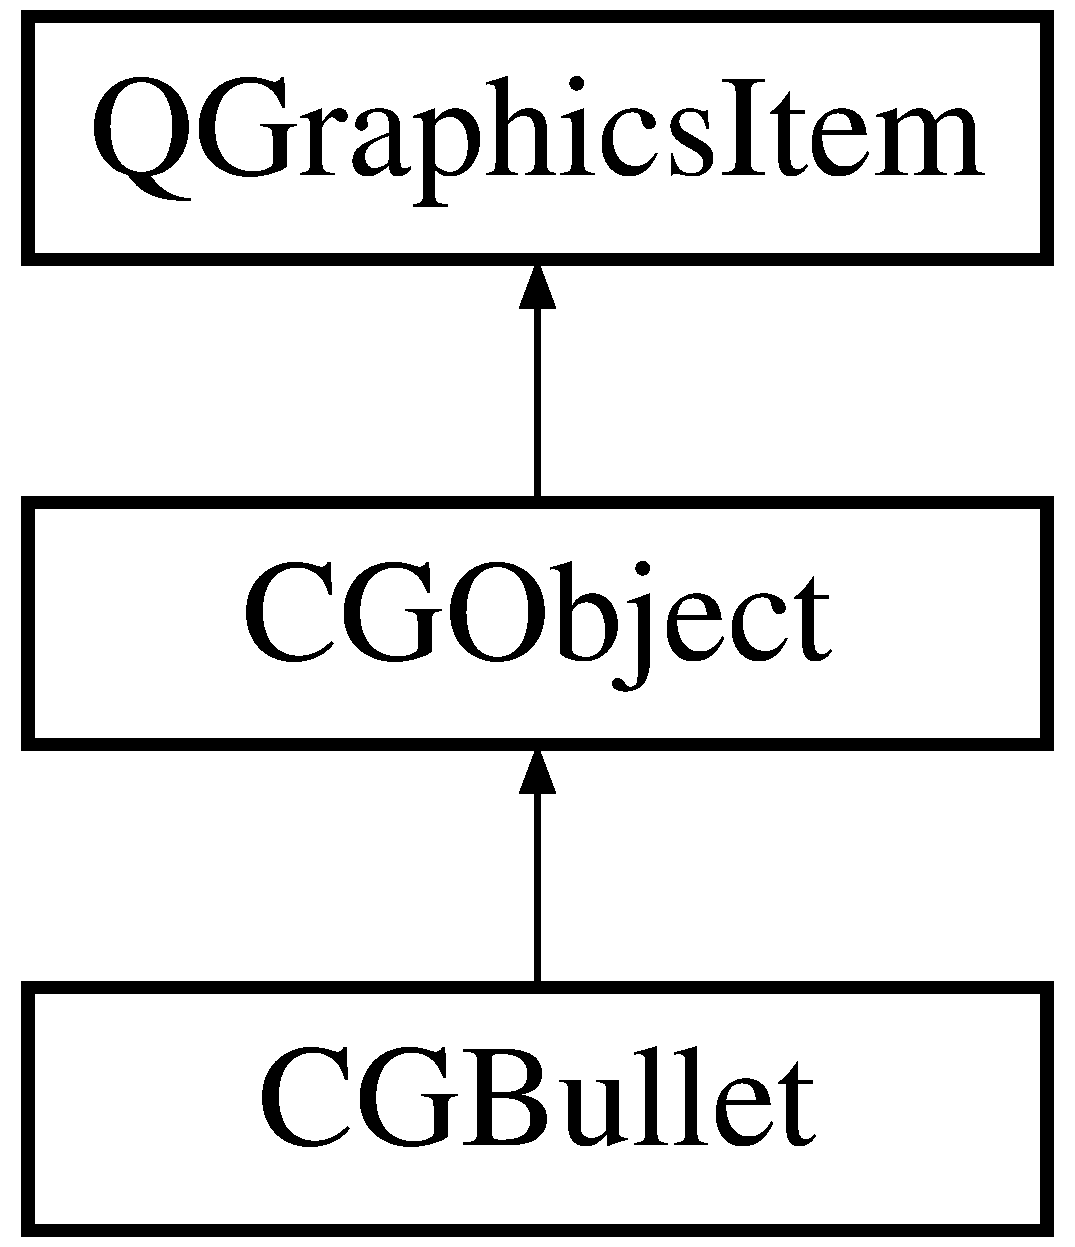
\includegraphics[height=3.000000cm]{class_c_g_bullet}
\end{center}
\end{figure}
\subsection*{Public Member Functions}
\begin{DoxyCompactItemize}
\item 
\mbox{\hyperlink{class_c_g_bullet_adb7c1130f83ecdbf16586a5e4adbca0b}{C\+G\+Bullet}} (\mbox{\hyperlink{class_c_object}{C\+Object}} $\ast$o)
\item 
void \mbox{\hyperlink{class_c_g_bullet_ad64e0666c42b0d65bb90ad37998252d0}{paint}} (Q\+Painter $\ast$painter, const Q\+Style\+Option\+Graphics\+Item $\ast$option, Q\+Widget $\ast$widget) override
\begin{DoxyCompactList}\small\item\em Funkcja określająca kształt obiektu, jej implementacja zależy od rodzaju klasy pochodnej. \end{DoxyCompactList}\item 
Q\+RectF \mbox{\hyperlink{class_c_g_bullet_a7be9c986a5c21d0a27dd5d64b209a82d}{bounding\+Rect}} () const override
\begin{DoxyCompactList}\small\item\em Zwraca prostokąt reprezentujący obrys obiektu; potrzebne do prawidłowego odświeżania obiektu na mapie; implementacja różna dla klas pochodnych. \end{DoxyCompactList}\item 
void \mbox{\hyperlink{class_c_g_bullet_a3f1f31f6225a94b09ea8493e5b2040a8}{advance}} () override
\begin{DoxyCompactList}\small\item\em Funkcja rysująca obiekt na mapie na podstawie parametrów obiektu logicznego. \end{DoxyCompactList}\item 
Q\+Painter\+Path \mbox{\hyperlink{class_c_g_bullet_a6e202930dce8f614c5acb55de035bda2}{shape}} () const override
\end{DoxyCompactItemize}
\subsection*{Additional Inherited Members}


\subsection{Detailed Description}
Graficzna reprezentacja pocisku. 

\subsection{Constructor \& Destructor Documentation}
\mbox{\Hypertarget{class_c_g_bullet_adb7c1130f83ecdbf16586a5e4adbca0b}\label{class_c_g_bullet_adb7c1130f83ecdbf16586a5e4adbca0b}} 
\index{C\+G\+Bullet@{C\+G\+Bullet}!C\+G\+Bullet@{C\+G\+Bullet}}
\index{C\+G\+Bullet@{C\+G\+Bullet}!C\+G\+Bullet@{C\+G\+Bullet}}
\subsubsection{\texorpdfstring{C\+G\+Bullet()}{CGBullet()}}
{\footnotesize\ttfamily C\+G\+Bullet\+::\+C\+G\+Bullet (\begin{DoxyParamCaption}\item[{\mbox{\hyperlink{class_c_object}{C\+Object}} $\ast$}]{o }\end{DoxyParamCaption})}



\subsection{Member Function Documentation}
\mbox{\Hypertarget{class_c_g_bullet_a3f1f31f6225a94b09ea8493e5b2040a8}\label{class_c_g_bullet_a3f1f31f6225a94b09ea8493e5b2040a8}} 
\index{C\+G\+Bullet@{C\+G\+Bullet}!advance@{advance}}
\index{advance@{advance}!C\+G\+Bullet@{C\+G\+Bullet}}
\subsubsection{\texorpdfstring{advance()}{advance()}}
{\footnotesize\ttfamily void C\+G\+Bullet\+::advance (\begin{DoxyParamCaption}{ }\end{DoxyParamCaption})\hspace{0.3cm}{\ttfamily [override]}, {\ttfamily [virtual]}}



Funkcja rysująca obiekt na mapie na podstawie parametrów obiektu logicznego. 



Implements \mbox{\hyperlink{class_c_g_object_a859e765fbb3ab0d6ad73ca58e5e49779}{C\+G\+Object}}.

\mbox{\Hypertarget{class_c_g_bullet_a7be9c986a5c21d0a27dd5d64b209a82d}\label{class_c_g_bullet_a7be9c986a5c21d0a27dd5d64b209a82d}} 
\index{C\+G\+Bullet@{C\+G\+Bullet}!bounding\+Rect@{bounding\+Rect}}
\index{bounding\+Rect@{bounding\+Rect}!C\+G\+Bullet@{C\+G\+Bullet}}
\subsubsection{\texorpdfstring{bounding\+Rect()}{boundingRect()}}
{\footnotesize\ttfamily Q\+RectF C\+G\+Bullet\+::bounding\+Rect (\begin{DoxyParamCaption}{ }\end{DoxyParamCaption}) const\hspace{0.3cm}{\ttfamily [override]}, {\ttfamily [virtual]}}



Zwraca prostokąt reprezentujący obrys obiektu; potrzebne do prawidłowego odświeżania obiektu na mapie; implementacja różna dla klas pochodnych. 

\begin{DoxyReturn}{Returns}
Q\+RecF reprezentujący obrys obiektu 
\end{DoxyReturn}


Implements \mbox{\hyperlink{class_c_g_object_ab9edf3d10a53c254cdb5d3d8de930207}{C\+G\+Object}}.

\mbox{\Hypertarget{class_c_g_bullet_ad64e0666c42b0d65bb90ad37998252d0}\label{class_c_g_bullet_ad64e0666c42b0d65bb90ad37998252d0}} 
\index{C\+G\+Bullet@{C\+G\+Bullet}!paint@{paint}}
\index{paint@{paint}!C\+G\+Bullet@{C\+G\+Bullet}}
\subsubsection{\texorpdfstring{paint()}{paint()}}
{\footnotesize\ttfamily void C\+G\+Bullet\+::paint (\begin{DoxyParamCaption}\item[{Q\+Painter $\ast$}]{painter,  }\item[{const Q\+Style\+Option\+Graphics\+Item $\ast$}]{option,  }\item[{Q\+Widget $\ast$}]{widget }\end{DoxyParamCaption})\hspace{0.3cm}{\ttfamily [override]}, {\ttfamily [virtual]}}



Funkcja określająca kształt obiektu, jej implementacja zależy od rodzaju klasy pochodnej. 


\begin{DoxyParams}{Parameters}
{\em painter} & \\
\hline
{\em option} & \\
\hline
{\em widget} & \\
\hline
\end{DoxyParams}


Implements \mbox{\hyperlink{class_c_g_object_a9622c313eb09ca5fc0e34f5d2aaac910}{C\+G\+Object}}.

\mbox{\Hypertarget{class_c_g_bullet_a6e202930dce8f614c5acb55de035bda2}\label{class_c_g_bullet_a6e202930dce8f614c5acb55de035bda2}} 
\index{C\+G\+Bullet@{C\+G\+Bullet}!shape@{shape}}
\index{shape@{shape}!C\+G\+Bullet@{C\+G\+Bullet}}
\subsubsection{\texorpdfstring{shape()}{shape()}}
{\footnotesize\ttfamily Q\+Painter\+Path C\+G\+Bullet\+::shape (\begin{DoxyParamCaption}{ }\end{DoxyParamCaption}) const\hspace{0.3cm}{\ttfamily [override]}}



The documentation for this class was generated from the following files\+:\begin{DoxyCompactItemize}
\item 
\mbox{\hyperlink{cgbullet_8h}{cgbullet.\+h}}\item 
\mbox{\hyperlink{cgbullet_8cpp}{cgbullet.\+cpp}}\end{DoxyCompactItemize}

\hypertarget{class_c_g_cleaning_robot}{}\section{C\+G\+Cleaning\+Robot Class Reference}
\label{class_c_g_cleaning_robot}\index{C\+G\+Cleaning\+Robot@{C\+G\+Cleaning\+Robot}}


Graficzna reprezentacja robota czyszczącego.  




{\ttfamily \#include $<$cgcleaningrobot.\+h$>$}

Inheritance diagram for C\+G\+Cleaning\+Robot\+:\begin{figure}[H]
\begin{center}
\leavevmode
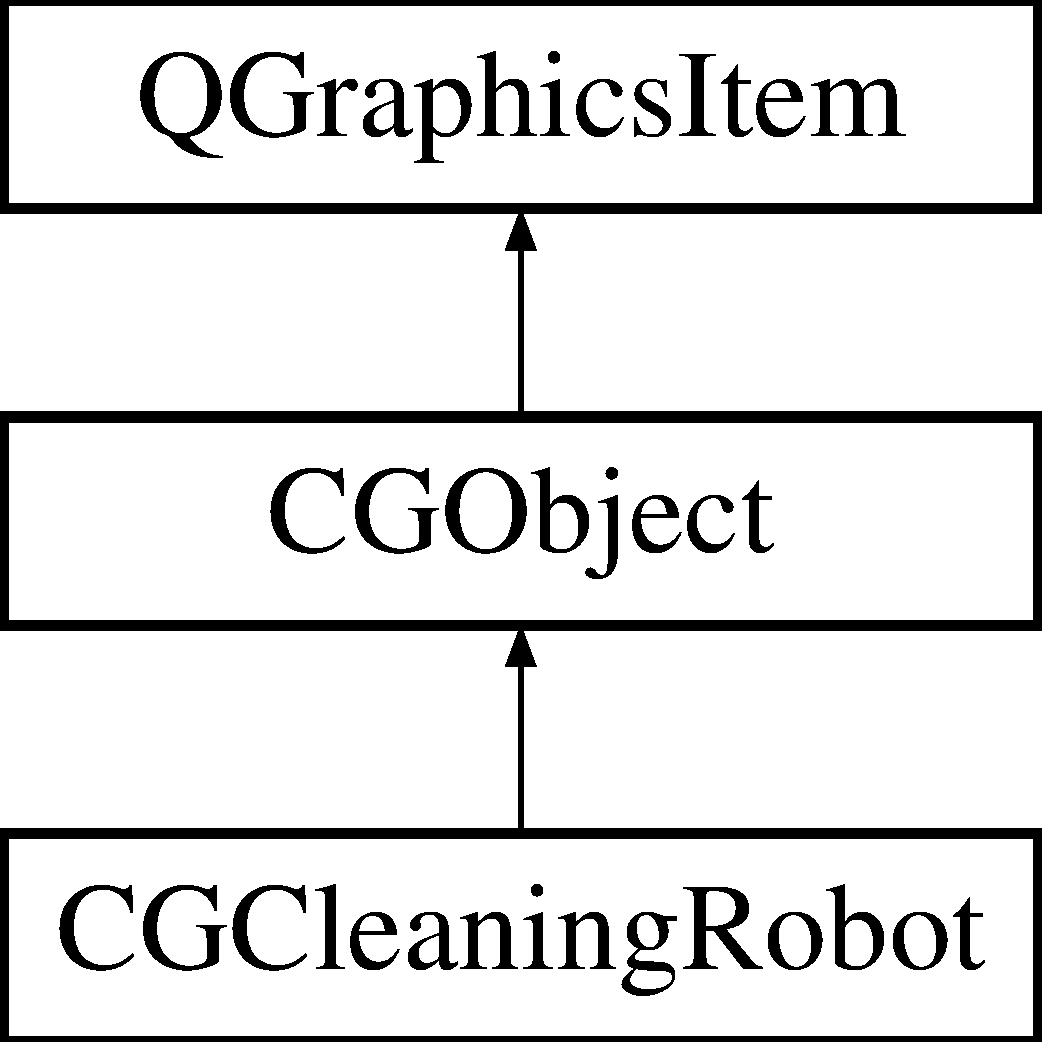
\includegraphics[height=3.000000cm]{class_c_g_cleaning_robot}
\end{center}
\end{figure}
\subsection*{Public Member Functions}
\begin{DoxyCompactItemize}
\item 
\mbox{\hyperlink{class_c_g_cleaning_robot_a5160e7e9a94c95ca091fab0375b8c414}{C\+G\+Cleaning\+Robot}} (\mbox{\hyperlink{class_c_object}{C\+Object}} $\ast$o)
\item 
void \mbox{\hyperlink{class_c_g_cleaning_robot_ad5c738dfd5633e0a4165309dd26033f5}{paint}} (Q\+Painter $\ast$painter, const Q\+Style\+Option\+Graphics\+Item $\ast$option, Q\+Widget $\ast$widget) override
\begin{DoxyCompactList}\small\item\em Funkcja określająca kształt obiektu, jej implementacja zależy od rodzaju klasy pochodnej. \end{DoxyCompactList}\item 
Q\+RectF \mbox{\hyperlink{class_c_g_cleaning_robot_a6fe8401e3b604cf5c3e449a56bb5655c}{bounding\+Rect}} () const override
\begin{DoxyCompactList}\small\item\em Zwraca prostokąt reprezentujący obrys obiektu; potrzebne do prawidłowego odświeżania obiektu na mapie; implementacja różna dla klas pochodnych. \end{DoxyCompactList}\item 
void \mbox{\hyperlink{class_c_g_cleaning_robot_a96511d40b48a6ac5a2fa31f2ed1f24e7}{advance}} () override
\begin{DoxyCompactList}\small\item\em Funkcja rysująca obiekt na mapie na podstawie parametrów obiektu logicznego. \end{DoxyCompactList}\item 
Q\+Painter\+Path \mbox{\hyperlink{class_c_g_cleaning_robot_a6ce1fefa61f2ffab1ec6c2ed2dad9ebe}{shape}} () const override
\end{DoxyCompactItemize}
\subsection*{Additional Inherited Members}


\subsection{Detailed Description}
Graficzna reprezentacja robota czyszczącego. 

\subsection{Constructor \& Destructor Documentation}
\mbox{\Hypertarget{class_c_g_cleaning_robot_a5160e7e9a94c95ca091fab0375b8c414}\label{class_c_g_cleaning_robot_a5160e7e9a94c95ca091fab0375b8c414}} 
\index{C\+G\+Cleaning\+Robot@{C\+G\+Cleaning\+Robot}!C\+G\+Cleaning\+Robot@{C\+G\+Cleaning\+Robot}}
\index{C\+G\+Cleaning\+Robot@{C\+G\+Cleaning\+Robot}!C\+G\+Cleaning\+Robot@{C\+G\+Cleaning\+Robot}}
\subsubsection{\texorpdfstring{C\+G\+Cleaning\+Robot()}{CGCleaningRobot()}}
{\footnotesize\ttfamily C\+G\+Cleaning\+Robot\+::\+C\+G\+Cleaning\+Robot (\begin{DoxyParamCaption}\item[{\mbox{\hyperlink{class_c_object}{C\+Object}} $\ast$}]{o }\end{DoxyParamCaption})}



\subsection{Member Function Documentation}
\mbox{\Hypertarget{class_c_g_cleaning_robot_a96511d40b48a6ac5a2fa31f2ed1f24e7}\label{class_c_g_cleaning_robot_a96511d40b48a6ac5a2fa31f2ed1f24e7}} 
\index{C\+G\+Cleaning\+Robot@{C\+G\+Cleaning\+Robot}!advance@{advance}}
\index{advance@{advance}!C\+G\+Cleaning\+Robot@{C\+G\+Cleaning\+Robot}}
\subsubsection{\texorpdfstring{advance()}{advance()}}
{\footnotesize\ttfamily void C\+G\+Cleaning\+Robot\+::advance (\begin{DoxyParamCaption}{ }\end{DoxyParamCaption})\hspace{0.3cm}{\ttfamily [override]}, {\ttfamily [virtual]}}



Funkcja rysująca obiekt na mapie na podstawie parametrów obiektu logicznego. 



Implements \mbox{\hyperlink{class_c_g_object_a859e765fbb3ab0d6ad73ca58e5e49779}{C\+G\+Object}}.

\mbox{\Hypertarget{class_c_g_cleaning_robot_a6fe8401e3b604cf5c3e449a56bb5655c}\label{class_c_g_cleaning_robot_a6fe8401e3b604cf5c3e449a56bb5655c}} 
\index{C\+G\+Cleaning\+Robot@{C\+G\+Cleaning\+Robot}!bounding\+Rect@{bounding\+Rect}}
\index{bounding\+Rect@{bounding\+Rect}!C\+G\+Cleaning\+Robot@{C\+G\+Cleaning\+Robot}}
\subsubsection{\texorpdfstring{bounding\+Rect()}{boundingRect()}}
{\footnotesize\ttfamily Q\+RectF C\+G\+Cleaning\+Robot\+::bounding\+Rect (\begin{DoxyParamCaption}{ }\end{DoxyParamCaption}) const\hspace{0.3cm}{\ttfamily [override]}, {\ttfamily [virtual]}}



Zwraca prostokąt reprezentujący obrys obiektu; potrzebne do prawidłowego odświeżania obiektu na mapie; implementacja różna dla klas pochodnych. 

\begin{DoxyReturn}{Returns}
Q\+RecF reprezentujący obrys obiektu 
\end{DoxyReturn}


Implements \mbox{\hyperlink{class_c_g_object_ab9edf3d10a53c254cdb5d3d8de930207}{C\+G\+Object}}.

\mbox{\Hypertarget{class_c_g_cleaning_robot_ad5c738dfd5633e0a4165309dd26033f5}\label{class_c_g_cleaning_robot_ad5c738dfd5633e0a4165309dd26033f5}} 
\index{C\+G\+Cleaning\+Robot@{C\+G\+Cleaning\+Robot}!paint@{paint}}
\index{paint@{paint}!C\+G\+Cleaning\+Robot@{C\+G\+Cleaning\+Robot}}
\subsubsection{\texorpdfstring{paint()}{paint()}}
{\footnotesize\ttfamily void C\+G\+Cleaning\+Robot\+::paint (\begin{DoxyParamCaption}\item[{Q\+Painter $\ast$}]{painter,  }\item[{const Q\+Style\+Option\+Graphics\+Item $\ast$}]{option,  }\item[{Q\+Widget $\ast$}]{widget }\end{DoxyParamCaption})\hspace{0.3cm}{\ttfamily [override]}, {\ttfamily [virtual]}}



Funkcja określająca kształt obiektu, jej implementacja zależy od rodzaju klasy pochodnej. 


\begin{DoxyParams}{Parameters}
{\em painter} & \\
\hline
{\em option} & \\
\hline
{\em widget} & \\
\hline
\end{DoxyParams}


Implements \mbox{\hyperlink{class_c_g_object_a9622c313eb09ca5fc0e34f5d2aaac910}{C\+G\+Object}}.

\mbox{\Hypertarget{class_c_g_cleaning_robot_a6ce1fefa61f2ffab1ec6c2ed2dad9ebe}\label{class_c_g_cleaning_robot_a6ce1fefa61f2ffab1ec6c2ed2dad9ebe}} 
\index{C\+G\+Cleaning\+Robot@{C\+G\+Cleaning\+Robot}!shape@{shape}}
\index{shape@{shape}!C\+G\+Cleaning\+Robot@{C\+G\+Cleaning\+Robot}}
\subsubsection{\texorpdfstring{shape()}{shape()}}
{\footnotesize\ttfamily Q\+Painter\+Path C\+G\+Cleaning\+Robot\+::shape (\begin{DoxyParamCaption}{ }\end{DoxyParamCaption}) const\hspace{0.3cm}{\ttfamily [override]}}



The documentation for this class was generated from the following files\+:\begin{DoxyCompactItemize}
\item 
\mbox{\hyperlink{cgcleaningrobot_8h}{cgcleaningrobot.\+h}}\item 
\mbox{\hyperlink{cgcleaningrobot_8cpp}{cgcleaningrobot.\+cpp}}\end{DoxyCompactItemize}

\hypertarget{class_c_g_dirt}{}\section{C\+G\+Dirt Class Reference}
\label{class_c_g_dirt}\index{C\+G\+Dirt@{C\+G\+Dirt}}


Graficzna reprezentacja brudu.  




{\ttfamily \#include $<$cgdirt.\+h$>$}

Inheritance diagram for C\+G\+Dirt\+:\begin{figure}[H]
\begin{center}
\leavevmode
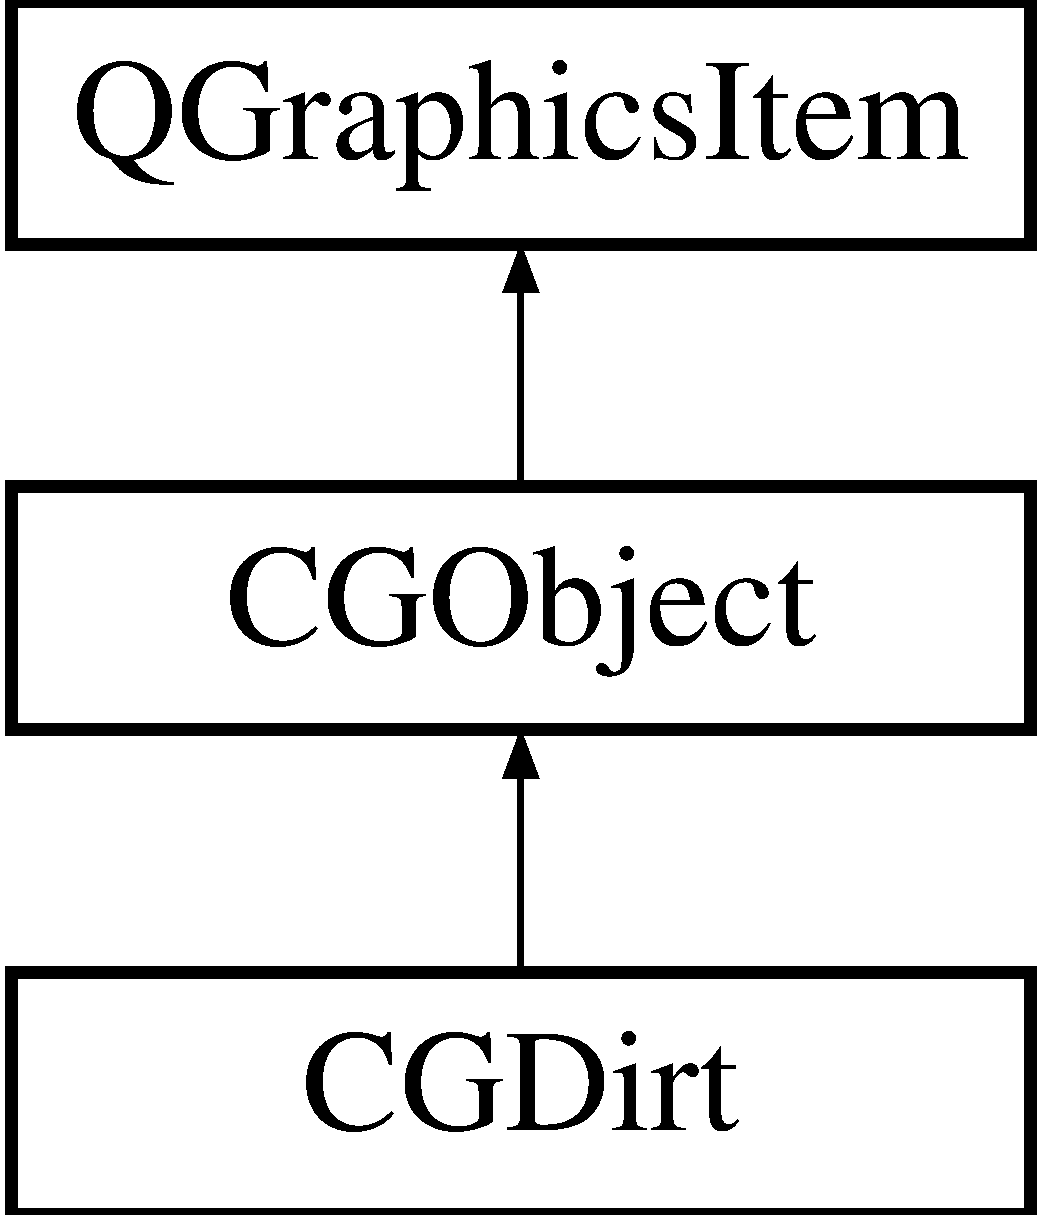
\includegraphics[height=3.000000cm]{class_c_g_dirt}
\end{center}
\end{figure}
\subsection*{Public Member Functions}
\begin{DoxyCompactItemize}
\item 
\mbox{\hyperlink{class_c_g_dirt_ad57eda78ac27258e3c951434bdbabcbb}{C\+G\+Dirt}} (\mbox{\hyperlink{class_c_object}{C\+Object}} $\ast$o)
\item 
void \mbox{\hyperlink{class_c_g_dirt_a46b019eb8693b85447149170178f8643}{paint}} (Q\+Painter $\ast$painter, const Q\+Style\+Option\+Graphics\+Item $\ast$option, Q\+Widget $\ast$widget) override
\begin{DoxyCompactList}\small\item\em Funkcja określająca kształt obiektu, jej implementacja zależy od rodzaju klasy pochodnej. \end{DoxyCompactList}\item 
Q\+RectF \mbox{\hyperlink{class_c_g_dirt_aa7ff4b489e4fdbdaa456b40394b635f1}{bounding\+Rect}} () const override
\begin{DoxyCompactList}\small\item\em Zwraca prostokąt reprezentujący obrys obiektu; potrzebne do prawidłowego odświeżania obiektu na mapie; implementacja różna dla klas pochodnych. \end{DoxyCompactList}\item 
void \mbox{\hyperlink{class_c_g_dirt_a871068d11fec47d09635b8992b11f7c9}{advance}} () override
\begin{DoxyCompactList}\small\item\em Funkcja rysująca obiekt na mapie na podstawie parametrów obiektu logicznego. \end{DoxyCompactList}\item 
Q\+Painter\+Path \mbox{\hyperlink{class_c_g_dirt_abb94f12edfcd4b6ff07b02ed1dea98f9}{shape}} () const override
\end{DoxyCompactItemize}
\subsection*{Additional Inherited Members}


\subsection{Detailed Description}
Graficzna reprezentacja brudu. 

\subsection{Constructor \& Destructor Documentation}
\mbox{\Hypertarget{class_c_g_dirt_ad57eda78ac27258e3c951434bdbabcbb}\label{class_c_g_dirt_ad57eda78ac27258e3c951434bdbabcbb}} 
\index{C\+G\+Dirt@{C\+G\+Dirt}!C\+G\+Dirt@{C\+G\+Dirt}}
\index{C\+G\+Dirt@{C\+G\+Dirt}!C\+G\+Dirt@{C\+G\+Dirt}}
\subsubsection{\texorpdfstring{C\+G\+Dirt()}{CGDirt()}}
{\footnotesize\ttfamily C\+G\+Dirt\+::\+C\+G\+Dirt (\begin{DoxyParamCaption}\item[{\mbox{\hyperlink{class_c_object}{C\+Object}} $\ast$}]{o }\end{DoxyParamCaption})}



\subsection{Member Function Documentation}
\mbox{\Hypertarget{class_c_g_dirt_a871068d11fec47d09635b8992b11f7c9}\label{class_c_g_dirt_a871068d11fec47d09635b8992b11f7c9}} 
\index{C\+G\+Dirt@{C\+G\+Dirt}!advance@{advance}}
\index{advance@{advance}!C\+G\+Dirt@{C\+G\+Dirt}}
\subsubsection{\texorpdfstring{advance()}{advance()}}
{\footnotesize\ttfamily void C\+G\+Dirt\+::advance (\begin{DoxyParamCaption}{ }\end{DoxyParamCaption})\hspace{0.3cm}{\ttfamily [override]}, {\ttfamily [virtual]}}



Funkcja rysująca obiekt na mapie na podstawie parametrów obiektu logicznego. 



Implements \mbox{\hyperlink{class_c_g_object_a859e765fbb3ab0d6ad73ca58e5e49779}{C\+G\+Object}}.

\mbox{\Hypertarget{class_c_g_dirt_aa7ff4b489e4fdbdaa456b40394b635f1}\label{class_c_g_dirt_aa7ff4b489e4fdbdaa456b40394b635f1}} 
\index{C\+G\+Dirt@{C\+G\+Dirt}!bounding\+Rect@{bounding\+Rect}}
\index{bounding\+Rect@{bounding\+Rect}!C\+G\+Dirt@{C\+G\+Dirt}}
\subsubsection{\texorpdfstring{bounding\+Rect()}{boundingRect()}}
{\footnotesize\ttfamily Q\+RectF C\+G\+Dirt\+::bounding\+Rect (\begin{DoxyParamCaption}{ }\end{DoxyParamCaption}) const\hspace{0.3cm}{\ttfamily [override]}, {\ttfamily [virtual]}}



Zwraca prostokąt reprezentujący obrys obiektu; potrzebne do prawidłowego odświeżania obiektu na mapie; implementacja różna dla klas pochodnych. 

\begin{DoxyReturn}{Returns}
Q\+RecF reprezentujący obrys obiektu 
\end{DoxyReturn}


Implements \mbox{\hyperlink{class_c_g_object_ab9edf3d10a53c254cdb5d3d8de930207}{C\+G\+Object}}.

\mbox{\Hypertarget{class_c_g_dirt_a46b019eb8693b85447149170178f8643}\label{class_c_g_dirt_a46b019eb8693b85447149170178f8643}} 
\index{C\+G\+Dirt@{C\+G\+Dirt}!paint@{paint}}
\index{paint@{paint}!C\+G\+Dirt@{C\+G\+Dirt}}
\subsubsection{\texorpdfstring{paint()}{paint()}}
{\footnotesize\ttfamily void C\+G\+Dirt\+::paint (\begin{DoxyParamCaption}\item[{Q\+Painter $\ast$}]{painter,  }\item[{const Q\+Style\+Option\+Graphics\+Item $\ast$}]{option,  }\item[{Q\+Widget $\ast$}]{widget }\end{DoxyParamCaption})\hspace{0.3cm}{\ttfamily [override]}, {\ttfamily [virtual]}}



Funkcja określająca kształt obiektu, jej implementacja zależy od rodzaju klasy pochodnej. 


\begin{DoxyParams}{Parameters}
{\em painter} & \\
\hline
{\em option} & \\
\hline
{\em widget} & \\
\hline
\end{DoxyParams}


Implements \mbox{\hyperlink{class_c_g_object_a9622c313eb09ca5fc0e34f5d2aaac910}{C\+G\+Object}}.

\mbox{\Hypertarget{class_c_g_dirt_abb94f12edfcd4b6ff07b02ed1dea98f9}\label{class_c_g_dirt_abb94f12edfcd4b6ff07b02ed1dea98f9}} 
\index{C\+G\+Dirt@{C\+G\+Dirt}!shape@{shape}}
\index{shape@{shape}!C\+G\+Dirt@{C\+G\+Dirt}}
\subsubsection{\texorpdfstring{shape()}{shape()}}
{\footnotesize\ttfamily Q\+Painter\+Path C\+G\+Dirt\+::shape (\begin{DoxyParamCaption}{ }\end{DoxyParamCaption}) const\hspace{0.3cm}{\ttfamily [override]}}



The documentation for this class was generated from the following files\+:\begin{DoxyCompactItemize}
\item 
\mbox{\hyperlink{cgdirt_8h}{cgdirt.\+h}}\item 
\mbox{\hyperlink{cgdirt_8cpp}{cgdirt.\+cpp}}\end{DoxyCompactItemize}

\hypertarget{class_c_g_fighting_robot}{}\section{C\+G\+Fighting\+Robot Class Reference}
\label{class_c_g_fighting_robot}\index{C\+G\+Fighting\+Robot@{C\+G\+Fighting\+Robot}}


Graficzna reprezentacja robota walczącego.  




{\ttfamily \#include $<$cgfightingrobot.\+h$>$}

Inheritance diagram for C\+G\+Fighting\+Robot\+:\begin{figure}[H]
\begin{center}
\leavevmode
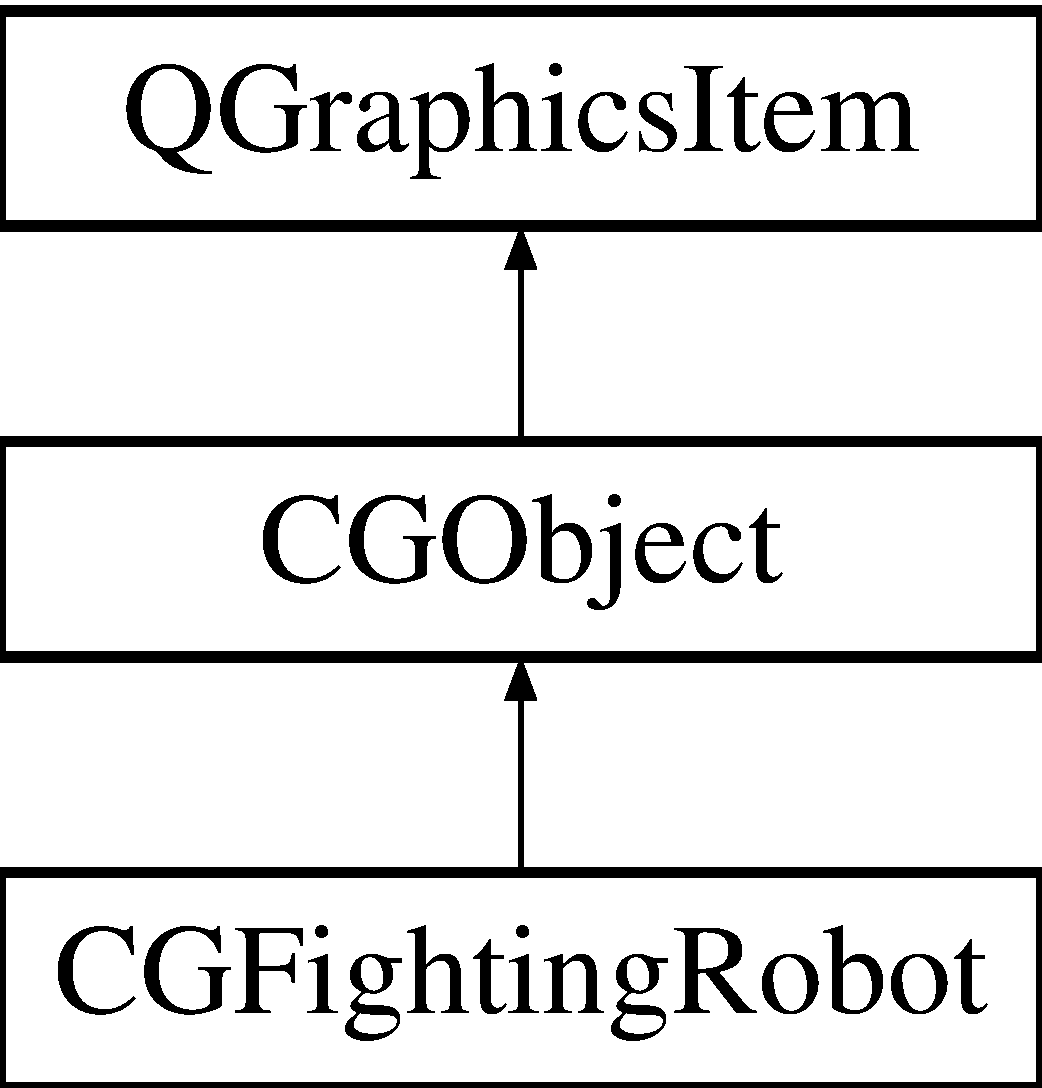
\includegraphics[height=3.000000cm]{class_c_g_fighting_robot}
\end{center}
\end{figure}
\subsection*{Public Member Functions}
\begin{DoxyCompactItemize}
\item 
\mbox{\hyperlink{class_c_g_fighting_robot_ae05396a82beb9769197b6295654dece5}{C\+G\+Fighting\+Robot}} (\mbox{\hyperlink{class_c_object}{C\+Object}} $\ast$o)
\item 
void \mbox{\hyperlink{class_c_g_fighting_robot_ad269a29840cb25ecb91f5a3c609ff4dd}{paint}} (Q\+Painter $\ast$painter, const Q\+Style\+Option\+Graphics\+Item $\ast$option, Q\+Widget $\ast$widget) override
\begin{DoxyCompactList}\small\item\em Funkcja określająca kształt obiektu, jej implementacja zależy od rodzaju klasy pochodnej. \end{DoxyCompactList}\item 
Q\+RectF \mbox{\hyperlink{class_c_g_fighting_robot_a945d974c6e61507a9f671ab7288df85a}{bounding\+Rect}} () const override
\begin{DoxyCompactList}\small\item\em Zwraca prostokąt reprezentujący obrys obiektu; potrzebne do prawidłowego odświeżania obiektu na mapie; implementacja różna dla klas pochodnych. \end{DoxyCompactList}\item 
void \mbox{\hyperlink{class_c_g_fighting_robot_aee1cbe4ebdf24953ff3a9def4338c283}{advance}} () override
\begin{DoxyCompactList}\small\item\em Funkcja rysująca obiekt na mapie na podstawie parametrów obiektu logicznego. \end{DoxyCompactList}\item 
Q\+Painter\+Path \mbox{\hyperlink{class_c_g_fighting_robot_a5ddec756ac208dd8f8044028b376ace9}{shape}} () const override
\end{DoxyCompactItemize}
\subsection*{Additional Inherited Members}


\subsection{Detailed Description}
Graficzna reprezentacja robota walczącego. 

\subsection{Constructor \& Destructor Documentation}
\mbox{\Hypertarget{class_c_g_fighting_robot_ae05396a82beb9769197b6295654dece5}\label{class_c_g_fighting_robot_ae05396a82beb9769197b6295654dece5}} 
\index{C\+G\+Fighting\+Robot@{C\+G\+Fighting\+Robot}!C\+G\+Fighting\+Robot@{C\+G\+Fighting\+Robot}}
\index{C\+G\+Fighting\+Robot@{C\+G\+Fighting\+Robot}!C\+G\+Fighting\+Robot@{C\+G\+Fighting\+Robot}}
\subsubsection{\texorpdfstring{C\+G\+Fighting\+Robot()}{CGFightingRobot()}}
{\footnotesize\ttfamily C\+G\+Fighting\+Robot\+::\+C\+G\+Fighting\+Robot (\begin{DoxyParamCaption}\item[{\mbox{\hyperlink{class_c_object}{C\+Object}} $\ast$}]{o }\end{DoxyParamCaption})}



\subsection{Member Function Documentation}
\mbox{\Hypertarget{class_c_g_fighting_robot_aee1cbe4ebdf24953ff3a9def4338c283}\label{class_c_g_fighting_robot_aee1cbe4ebdf24953ff3a9def4338c283}} 
\index{C\+G\+Fighting\+Robot@{C\+G\+Fighting\+Robot}!advance@{advance}}
\index{advance@{advance}!C\+G\+Fighting\+Robot@{C\+G\+Fighting\+Robot}}
\subsubsection{\texorpdfstring{advance()}{advance()}}
{\footnotesize\ttfamily void C\+G\+Fighting\+Robot\+::advance (\begin{DoxyParamCaption}{ }\end{DoxyParamCaption})\hspace{0.3cm}{\ttfamily [override]}, {\ttfamily [virtual]}}



Funkcja rysująca obiekt na mapie na podstawie parametrów obiektu logicznego. 



Implements \mbox{\hyperlink{class_c_g_object_a859e765fbb3ab0d6ad73ca58e5e49779}{C\+G\+Object}}.

\mbox{\Hypertarget{class_c_g_fighting_robot_a945d974c6e61507a9f671ab7288df85a}\label{class_c_g_fighting_robot_a945d974c6e61507a9f671ab7288df85a}} 
\index{C\+G\+Fighting\+Robot@{C\+G\+Fighting\+Robot}!bounding\+Rect@{bounding\+Rect}}
\index{bounding\+Rect@{bounding\+Rect}!C\+G\+Fighting\+Robot@{C\+G\+Fighting\+Robot}}
\subsubsection{\texorpdfstring{bounding\+Rect()}{boundingRect()}}
{\footnotesize\ttfamily Q\+RectF C\+G\+Fighting\+Robot\+::bounding\+Rect (\begin{DoxyParamCaption}{ }\end{DoxyParamCaption}) const\hspace{0.3cm}{\ttfamily [override]}, {\ttfamily [virtual]}}



Zwraca prostokąt reprezentujący obrys obiektu; potrzebne do prawidłowego odświeżania obiektu na mapie; implementacja różna dla klas pochodnych. 

\begin{DoxyReturn}{Returns}
Q\+RecF reprezentujący obrys obiektu 
\end{DoxyReturn}


Implements \mbox{\hyperlink{class_c_g_object_ab9edf3d10a53c254cdb5d3d8de930207}{C\+G\+Object}}.

\mbox{\Hypertarget{class_c_g_fighting_robot_ad269a29840cb25ecb91f5a3c609ff4dd}\label{class_c_g_fighting_robot_ad269a29840cb25ecb91f5a3c609ff4dd}} 
\index{C\+G\+Fighting\+Robot@{C\+G\+Fighting\+Robot}!paint@{paint}}
\index{paint@{paint}!C\+G\+Fighting\+Robot@{C\+G\+Fighting\+Robot}}
\subsubsection{\texorpdfstring{paint()}{paint()}}
{\footnotesize\ttfamily void C\+G\+Fighting\+Robot\+::paint (\begin{DoxyParamCaption}\item[{Q\+Painter $\ast$}]{painter,  }\item[{const Q\+Style\+Option\+Graphics\+Item $\ast$}]{option,  }\item[{Q\+Widget $\ast$}]{widget }\end{DoxyParamCaption})\hspace{0.3cm}{\ttfamily [override]}, {\ttfamily [virtual]}}



Funkcja określająca kształt obiektu, jej implementacja zależy od rodzaju klasy pochodnej. 


\begin{DoxyParams}{Parameters}
{\em painter} & \\
\hline
{\em option} & \\
\hline
{\em widget} & \\
\hline
\end{DoxyParams}


Implements \mbox{\hyperlink{class_c_g_object_a9622c313eb09ca5fc0e34f5d2aaac910}{C\+G\+Object}}.

\mbox{\Hypertarget{class_c_g_fighting_robot_a5ddec756ac208dd8f8044028b376ace9}\label{class_c_g_fighting_robot_a5ddec756ac208dd8f8044028b376ace9}} 
\index{C\+G\+Fighting\+Robot@{C\+G\+Fighting\+Robot}!shape@{shape}}
\index{shape@{shape}!C\+G\+Fighting\+Robot@{C\+G\+Fighting\+Robot}}
\subsubsection{\texorpdfstring{shape()}{shape()}}
{\footnotesize\ttfamily Q\+Painter\+Path C\+G\+Fighting\+Robot\+::shape (\begin{DoxyParamCaption}{ }\end{DoxyParamCaption}) const\hspace{0.3cm}{\ttfamily [override]}}



The documentation for this class was generated from the following files\+:\begin{DoxyCompactItemize}
\item 
\mbox{\hyperlink{cgfightingrobot_8h}{cgfightingrobot.\+h}}\item 
\mbox{\hyperlink{cgfightingrobot_8cpp}{cgfightingrobot.\+cpp}}\end{DoxyCompactItemize}

\hypertarget{class_c_g_mine}{}\section{C\+G\+Mine Class Reference}
\label{class_c_g_mine}\index{C\+G\+Mine@{C\+G\+Mine}}


Graficzna reprezentacja miny.  




{\ttfamily \#include $<$cgmine.\+h$>$}

Inheritance diagram for C\+G\+Mine\+:\begin{figure}[H]
\begin{center}
\leavevmode
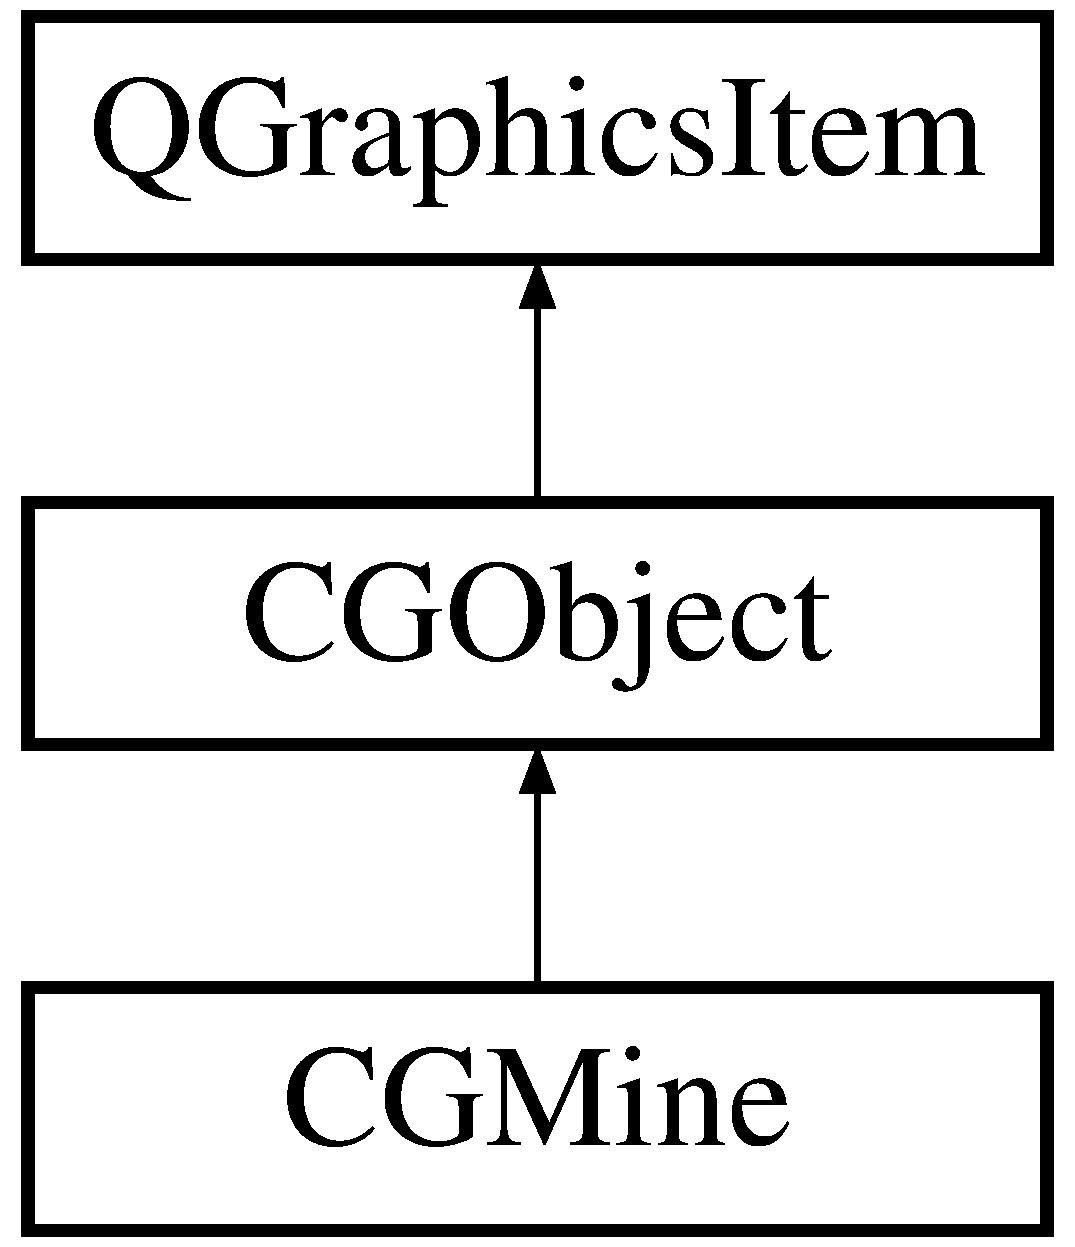
\includegraphics[height=3.000000cm]{class_c_g_mine}
\end{center}
\end{figure}
\subsection*{Public Member Functions}
\begin{DoxyCompactItemize}
\item 
\mbox{\hyperlink{class_c_g_mine_a2112f99209203ed64e398a2e358eb1cb}{C\+G\+Mine}} (\mbox{\hyperlink{class_c_object}{C\+Object}} $\ast$o)
\item 
void \mbox{\hyperlink{class_c_g_mine_a2a48415eeb9f9e662a068abd09f30b00}{paint}} (Q\+Painter $\ast$painter, const Q\+Style\+Option\+Graphics\+Item $\ast$option, Q\+Widget $\ast$widget) override
\begin{DoxyCompactList}\small\item\em Funkcja określająca kształt obiektu, jej implementacja zależy od rodzaju klasy pochodnej. \end{DoxyCompactList}\item 
Q\+RectF \mbox{\hyperlink{class_c_g_mine_ad11ed34f5cd02b51fd2baeaf700daba2}{bounding\+Rect}} () const override
\begin{DoxyCompactList}\small\item\em Zwraca prostokąt reprezentujący obrys obiektu; potrzebne do prawidłowego odświeżania obiektu na mapie; implementacja różna dla klas pochodnych. \end{DoxyCompactList}\item 
void \mbox{\hyperlink{class_c_g_mine_a6dbd841b39f421054cd8db54c3c84b74}{advance}} () override
\begin{DoxyCompactList}\small\item\em Funkcja rysująca obiekt na mapie na podstawie parametrów obiektu logicznego. \end{DoxyCompactList}\item 
Q\+Painter\+Path \mbox{\hyperlink{class_c_g_mine_aa0a9b3d1b7a092121033d2e2f519c09a}{shape}} () const override
\end{DoxyCompactItemize}
\subsection*{Additional Inherited Members}


\subsection{Detailed Description}
Graficzna reprezentacja miny. 

\subsection{Constructor \& Destructor Documentation}
\mbox{\Hypertarget{class_c_g_mine_a2112f99209203ed64e398a2e358eb1cb}\label{class_c_g_mine_a2112f99209203ed64e398a2e358eb1cb}} 
\index{C\+G\+Mine@{C\+G\+Mine}!C\+G\+Mine@{C\+G\+Mine}}
\index{C\+G\+Mine@{C\+G\+Mine}!C\+G\+Mine@{C\+G\+Mine}}
\subsubsection{\texorpdfstring{C\+G\+Mine()}{CGMine()}}
{\footnotesize\ttfamily C\+G\+Mine\+::\+C\+G\+Mine (\begin{DoxyParamCaption}\item[{\mbox{\hyperlink{class_c_object}{C\+Object}} $\ast$}]{o }\end{DoxyParamCaption})}



\subsection{Member Function Documentation}
\mbox{\Hypertarget{class_c_g_mine_a6dbd841b39f421054cd8db54c3c84b74}\label{class_c_g_mine_a6dbd841b39f421054cd8db54c3c84b74}} 
\index{C\+G\+Mine@{C\+G\+Mine}!advance@{advance}}
\index{advance@{advance}!C\+G\+Mine@{C\+G\+Mine}}
\subsubsection{\texorpdfstring{advance()}{advance()}}
{\footnotesize\ttfamily void C\+G\+Mine\+::advance (\begin{DoxyParamCaption}{ }\end{DoxyParamCaption})\hspace{0.3cm}{\ttfamily [override]}, {\ttfamily [virtual]}}



Funkcja rysująca obiekt na mapie na podstawie parametrów obiektu logicznego. 



Implements \mbox{\hyperlink{class_c_g_object_a859e765fbb3ab0d6ad73ca58e5e49779}{C\+G\+Object}}.

\mbox{\Hypertarget{class_c_g_mine_ad11ed34f5cd02b51fd2baeaf700daba2}\label{class_c_g_mine_ad11ed34f5cd02b51fd2baeaf700daba2}} 
\index{C\+G\+Mine@{C\+G\+Mine}!bounding\+Rect@{bounding\+Rect}}
\index{bounding\+Rect@{bounding\+Rect}!C\+G\+Mine@{C\+G\+Mine}}
\subsubsection{\texorpdfstring{bounding\+Rect()}{boundingRect()}}
{\footnotesize\ttfamily Q\+RectF C\+G\+Mine\+::bounding\+Rect (\begin{DoxyParamCaption}{ }\end{DoxyParamCaption}) const\hspace{0.3cm}{\ttfamily [override]}, {\ttfamily [virtual]}}



Zwraca prostokąt reprezentujący obrys obiektu; potrzebne do prawidłowego odświeżania obiektu na mapie; implementacja różna dla klas pochodnych. 

\begin{DoxyReturn}{Returns}
Q\+RecF reprezentujący obrys obiektu 
\end{DoxyReturn}


Implements \mbox{\hyperlink{class_c_g_object_ab9edf3d10a53c254cdb5d3d8de930207}{C\+G\+Object}}.

\mbox{\Hypertarget{class_c_g_mine_a2a48415eeb9f9e662a068abd09f30b00}\label{class_c_g_mine_a2a48415eeb9f9e662a068abd09f30b00}} 
\index{C\+G\+Mine@{C\+G\+Mine}!paint@{paint}}
\index{paint@{paint}!C\+G\+Mine@{C\+G\+Mine}}
\subsubsection{\texorpdfstring{paint()}{paint()}}
{\footnotesize\ttfamily void C\+G\+Mine\+::paint (\begin{DoxyParamCaption}\item[{Q\+Painter $\ast$}]{painter,  }\item[{const Q\+Style\+Option\+Graphics\+Item $\ast$}]{option,  }\item[{Q\+Widget $\ast$}]{widget }\end{DoxyParamCaption})\hspace{0.3cm}{\ttfamily [override]}, {\ttfamily [virtual]}}



Funkcja określająca kształt obiektu, jej implementacja zależy od rodzaju klasy pochodnej. 


\begin{DoxyParams}{Parameters}
{\em painter} & \\
\hline
{\em option} & \\
\hline
{\em widget} & \\
\hline
\end{DoxyParams}


Implements \mbox{\hyperlink{class_c_g_object_a9622c313eb09ca5fc0e34f5d2aaac910}{C\+G\+Object}}.

\mbox{\Hypertarget{class_c_g_mine_aa0a9b3d1b7a092121033d2e2f519c09a}\label{class_c_g_mine_aa0a9b3d1b7a092121033d2e2f519c09a}} 
\index{C\+G\+Mine@{C\+G\+Mine}!shape@{shape}}
\index{shape@{shape}!C\+G\+Mine@{C\+G\+Mine}}
\subsubsection{\texorpdfstring{shape()}{shape()}}
{\footnotesize\ttfamily Q\+Painter\+Path C\+G\+Mine\+::shape (\begin{DoxyParamCaption}{ }\end{DoxyParamCaption}) const\hspace{0.3cm}{\ttfamily [override]}}



The documentation for this class was generated from the following files\+:\begin{DoxyCompactItemize}
\item 
\mbox{\hyperlink{cgmine_8h}{cgmine.\+h}}\item 
\mbox{\hyperlink{cgmine_8cpp}{cgmine.\+cpp}}\end{DoxyCompactItemize}

\hypertarget{class_c_g_object}{}\section{C\+G\+Object Class Reference}
\label{class_c_g_object}\index{C\+G\+Object@{C\+G\+Object}}


Klasa służąca do wyświetlania na mapie obiektów logicznych.  




{\ttfamily \#include $<$cgobject.\+h$>$}

Inheritance diagram for C\+G\+Object\+:\begin{figure}[H]
\begin{center}
\leavevmode
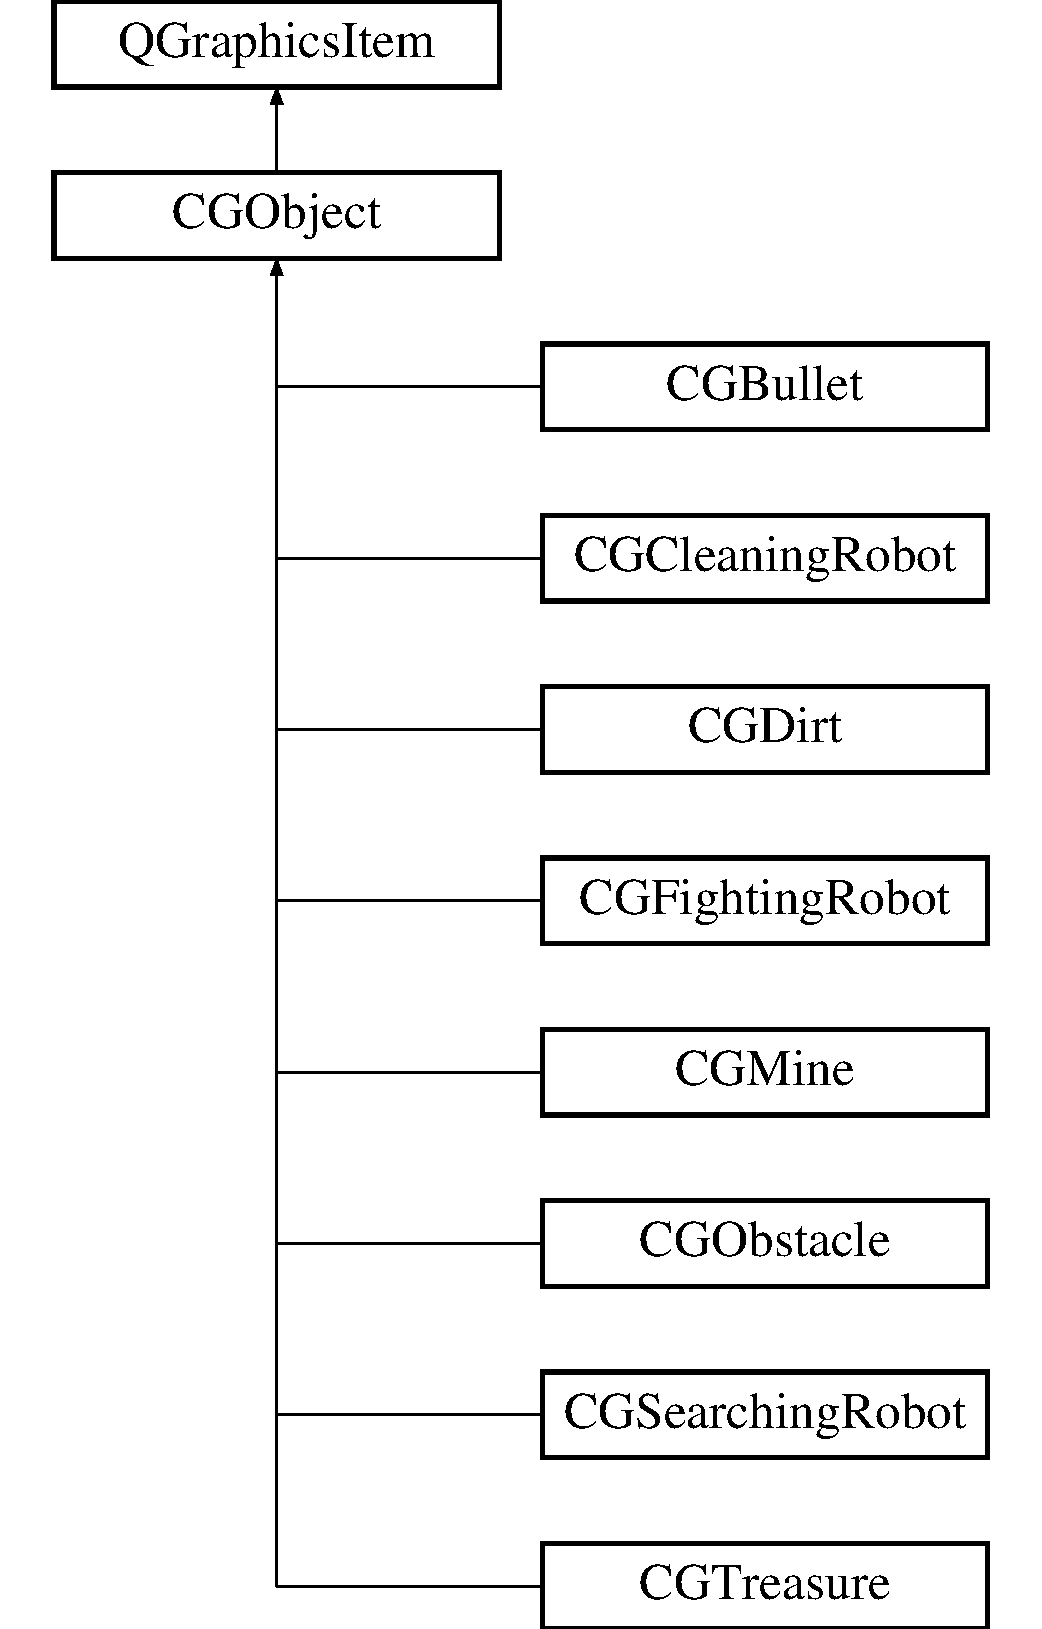
\includegraphics[height=10.000000cm]{class_c_g_object}
\end{center}
\end{figure}
\subsection*{Public Member Functions}
\begin{DoxyCompactItemize}
\item 
\mbox{\hyperlink{class_c_g_object_a40a7f41342b3b791a8854b3397378d5d}{C\+G\+Object}} (\mbox{\hyperlink{class_c_object}{C\+Object}} $\ast$o)
\begin{DoxyCompactList}\small\item\em Obiekt graficzny zawsze inicjalizowany jest wskaźnikiem na obiekt logiczny, który reprezentuje; wskaźnik na mapę pobierany jest z obiektu logicznego. \end{DoxyCompactList}\item 
\mbox{\hyperlink{class_c_object}{C\+Object}} $\ast$ \mbox{\hyperlink{class_c_g_object_a6e749272ebf5a43d43927cdfed21c46c}{get\+C\+Object}} ()
\begin{DoxyCompactList}\small\item\em Zwraca wskaźnik do obiektu logicznego reprezentowanego przez dany obiekt graficzny. \end{DoxyCompactList}\item 
virtual void \mbox{\hyperlink{class_c_g_object_a859e765fbb3ab0d6ad73ca58e5e49779}{advance}} ()=0
\begin{DoxyCompactList}\small\item\em Funkcja rysująca obiekt na mapie na podstawie parametrów obiektu logicznego. \end{DoxyCompactList}\item 
virtual Q\+RectF \mbox{\hyperlink{class_c_g_object_ab9edf3d10a53c254cdb5d3d8de930207}{bounding\+Rect}} () const =0
\begin{DoxyCompactList}\small\item\em Zwraca prostokąt reprezentujący obrys obiektu; potrzebne do prawidłowego odświeżania obiektu na mapie; implementacja różna dla klas pochodnych. \end{DoxyCompactList}\item 
virtual void \mbox{\hyperlink{class_c_g_object_a9622c313eb09ca5fc0e34f5d2aaac910}{paint}} (Q\+Painter $\ast$painter, const Q\+Style\+Option\+Graphics\+Item $\ast$option, Q\+Widget $\ast$widget)=0
\begin{DoxyCompactList}\small\item\em Funkcja określająca kształt obiektu, jej implementacja zależy od rodzaju klasy pochodnej. \end{DoxyCompactList}\end{DoxyCompactItemize}
\subsection*{Protected Attributes}
\begin{DoxyCompactItemize}
\item 
\mbox{\hyperlink{class_c_object}{C\+Object}} $\ast$ \mbox{\hyperlink{class_c_g_object_a8955574357e33ce28957c4ff42154cfb}{object}}
\begin{DoxyCompactList}\small\item\em Obiekt logiczny, którego reprezentacją jest dany obiekt graficzny. \end{DoxyCompactList}\item 
\mbox{\hyperlink{class_c_map}{C\+Map}} $\ast$ \mbox{\hyperlink{class_c_g_object_a8cfd8e7d917cd445ea8f5284f709452d}{map}}
\begin{DoxyCompactList}\small\item\em Wskaźnik na mapę, na której znajduje się obiekt graficzny. \end{DoxyCompactList}\end{DoxyCompactItemize}


\subsection{Detailed Description}
Klasa służąca do wyświetlania na mapie obiektów logicznych. 

\subsection{Constructor \& Destructor Documentation}
\mbox{\Hypertarget{class_c_g_object_a40a7f41342b3b791a8854b3397378d5d}\label{class_c_g_object_a40a7f41342b3b791a8854b3397378d5d}} 
\index{C\+G\+Object@{C\+G\+Object}!C\+G\+Object@{C\+G\+Object}}
\index{C\+G\+Object@{C\+G\+Object}!C\+G\+Object@{C\+G\+Object}}
\subsubsection{\texorpdfstring{C\+G\+Object()}{CGObject()}}
{\footnotesize\ttfamily C\+G\+Object\+::\+C\+G\+Object (\begin{DoxyParamCaption}\item[{\mbox{\hyperlink{class_c_object}{C\+Object}} $\ast$}]{o }\end{DoxyParamCaption})}



Obiekt graficzny zawsze inicjalizowany jest wskaźnikiem na obiekt logiczny, który reprezentuje; wskaźnik na mapę pobierany jest z obiektu logicznego. 


\begin{DoxyParams}{Parameters}
{\em o} & Obiekt logiczny, który ma być reprezentowany \\
\hline
\end{DoxyParams}


\subsection{Member Function Documentation}
\mbox{\Hypertarget{class_c_g_object_a859e765fbb3ab0d6ad73ca58e5e49779}\label{class_c_g_object_a859e765fbb3ab0d6ad73ca58e5e49779}} 
\index{C\+G\+Object@{C\+G\+Object}!advance@{advance}}
\index{advance@{advance}!C\+G\+Object@{C\+G\+Object}}
\subsubsection{\texorpdfstring{advance()}{advance()}}
{\footnotesize\ttfamily virtual void C\+G\+Object\+::advance (\begin{DoxyParamCaption}{ }\end{DoxyParamCaption})\hspace{0.3cm}{\ttfamily [pure virtual]}}



Funkcja rysująca obiekt na mapie na podstawie parametrów obiektu logicznego. 



Implemented in \mbox{\hyperlink{class_c_g_bullet_a3f1f31f6225a94b09ea8493e5b2040a8}{C\+G\+Bullet}}, \mbox{\hyperlink{class_c_g_cleaning_robot_a96511d40b48a6ac5a2fa31f2ed1f24e7}{C\+G\+Cleaning\+Robot}}, \mbox{\hyperlink{class_c_g_dirt_a871068d11fec47d09635b8992b11f7c9}{C\+G\+Dirt}}, \mbox{\hyperlink{class_c_g_fighting_robot_aee1cbe4ebdf24953ff3a9def4338c283}{C\+G\+Fighting\+Robot}}, \mbox{\hyperlink{class_c_g_mine_a6dbd841b39f421054cd8db54c3c84b74}{C\+G\+Mine}}, \mbox{\hyperlink{class_c_g_obstacle_adeb38e94e73f2c3d5d84afbb5e5e0fe7}{C\+G\+Obstacle}}, \mbox{\hyperlink{class_c_g_searching_robot_adcc4b3096e11c25287806428119acb22}{C\+G\+Searching\+Robot}}, and \mbox{\hyperlink{class_c_g_treasure_a4b8a13bcae320e63a87a32a804606190}{C\+G\+Treasure}}.

\mbox{\Hypertarget{class_c_g_object_ab9edf3d10a53c254cdb5d3d8de930207}\label{class_c_g_object_ab9edf3d10a53c254cdb5d3d8de930207}} 
\index{C\+G\+Object@{C\+G\+Object}!bounding\+Rect@{bounding\+Rect}}
\index{bounding\+Rect@{bounding\+Rect}!C\+G\+Object@{C\+G\+Object}}
\subsubsection{\texorpdfstring{bounding\+Rect()}{boundingRect()}}
{\footnotesize\ttfamily virtual Q\+RectF C\+G\+Object\+::bounding\+Rect (\begin{DoxyParamCaption}{ }\end{DoxyParamCaption}) const\hspace{0.3cm}{\ttfamily [pure virtual]}}



Zwraca prostokąt reprezentujący obrys obiektu; potrzebne do prawidłowego odświeżania obiektu na mapie; implementacja różna dla klas pochodnych. 

\begin{DoxyReturn}{Returns}
Q\+RecF reprezentujący obrys obiektu 
\end{DoxyReturn}


Implemented in \mbox{\hyperlink{class_c_g_bullet_a7be9c986a5c21d0a27dd5d64b209a82d}{C\+G\+Bullet}}, \mbox{\hyperlink{class_c_g_cleaning_robot_a6fe8401e3b604cf5c3e449a56bb5655c}{C\+G\+Cleaning\+Robot}}, \mbox{\hyperlink{class_c_g_dirt_aa7ff4b489e4fdbdaa456b40394b635f1}{C\+G\+Dirt}}, \mbox{\hyperlink{class_c_g_fighting_robot_a945d974c6e61507a9f671ab7288df85a}{C\+G\+Fighting\+Robot}}, \mbox{\hyperlink{class_c_g_mine_ad11ed34f5cd02b51fd2baeaf700daba2}{C\+G\+Mine}}, \mbox{\hyperlink{class_c_g_obstacle_a88a124737ae6f96c6b07316591ecdb34}{C\+G\+Obstacle}}, \mbox{\hyperlink{class_c_g_searching_robot_aa0cf51f6acdfa865c130f0cd16860625}{C\+G\+Searching\+Robot}}, and \mbox{\hyperlink{class_c_g_treasure_a103be7d49202d07d9260917a7d6e8429}{C\+G\+Treasure}}.

\mbox{\Hypertarget{class_c_g_object_a6e749272ebf5a43d43927cdfed21c46c}\label{class_c_g_object_a6e749272ebf5a43d43927cdfed21c46c}} 
\index{C\+G\+Object@{C\+G\+Object}!get\+C\+Object@{get\+C\+Object}}
\index{get\+C\+Object@{get\+C\+Object}!C\+G\+Object@{C\+G\+Object}}
\subsubsection{\texorpdfstring{get\+C\+Object()}{getCObject()}}
{\footnotesize\ttfamily \mbox{\hyperlink{class_c_object}{C\+Object}} $\ast$ C\+G\+Object\+::get\+C\+Object (\begin{DoxyParamCaption}{ }\end{DoxyParamCaption})}



Zwraca wskaźnik do obiektu logicznego reprezentowanego przez dany obiekt graficzny. 

\begin{DoxyReturn}{Returns}
object 
\end{DoxyReturn}
\mbox{\Hypertarget{class_c_g_object_a9622c313eb09ca5fc0e34f5d2aaac910}\label{class_c_g_object_a9622c313eb09ca5fc0e34f5d2aaac910}} 
\index{C\+G\+Object@{C\+G\+Object}!paint@{paint}}
\index{paint@{paint}!C\+G\+Object@{C\+G\+Object}}
\subsubsection{\texorpdfstring{paint()}{paint()}}
{\footnotesize\ttfamily virtual void C\+G\+Object\+::paint (\begin{DoxyParamCaption}\item[{Q\+Painter $\ast$}]{painter,  }\item[{const Q\+Style\+Option\+Graphics\+Item $\ast$}]{option,  }\item[{Q\+Widget $\ast$}]{widget }\end{DoxyParamCaption})\hspace{0.3cm}{\ttfamily [pure virtual]}}



Funkcja określająca kształt obiektu, jej implementacja zależy od rodzaju klasy pochodnej. 


\begin{DoxyParams}{Parameters}
{\em painter} & \\
\hline
{\em option} & \\
\hline
{\em widget} & \\
\hline
\end{DoxyParams}


Implemented in \mbox{\hyperlink{class_c_g_bullet_ad64e0666c42b0d65bb90ad37998252d0}{C\+G\+Bullet}}, \mbox{\hyperlink{class_c_g_cleaning_robot_ad5c738dfd5633e0a4165309dd26033f5}{C\+G\+Cleaning\+Robot}}, \mbox{\hyperlink{class_c_g_dirt_a46b019eb8693b85447149170178f8643}{C\+G\+Dirt}}, \mbox{\hyperlink{class_c_g_fighting_robot_ad269a29840cb25ecb91f5a3c609ff4dd}{C\+G\+Fighting\+Robot}}, \mbox{\hyperlink{class_c_g_mine_a2a48415eeb9f9e662a068abd09f30b00}{C\+G\+Mine}}, \mbox{\hyperlink{class_c_g_obstacle_a4ae41138f5fa9f7929c71f1999df7793}{C\+G\+Obstacle}}, \mbox{\hyperlink{class_c_g_searching_robot_ad6e9d94604256cb9f0fe6e708c4391ad}{C\+G\+Searching\+Robot}}, and \mbox{\hyperlink{class_c_g_treasure_aeab69a95590acb46aa4d20422be96560}{C\+G\+Treasure}}.



\subsection{Member Data Documentation}
\mbox{\Hypertarget{class_c_g_object_a8cfd8e7d917cd445ea8f5284f709452d}\label{class_c_g_object_a8cfd8e7d917cd445ea8f5284f709452d}} 
\index{C\+G\+Object@{C\+G\+Object}!map@{map}}
\index{map@{map}!C\+G\+Object@{C\+G\+Object}}
\subsubsection{\texorpdfstring{map}{map}}
{\footnotesize\ttfamily \mbox{\hyperlink{class_c_map}{C\+Map}}$\ast$ C\+G\+Object\+::map\hspace{0.3cm}{\ttfamily [protected]}}



Wskaźnik na mapę, na której znajduje się obiekt graficzny. 

\mbox{\Hypertarget{class_c_g_object_a8955574357e33ce28957c4ff42154cfb}\label{class_c_g_object_a8955574357e33ce28957c4ff42154cfb}} 
\index{C\+G\+Object@{C\+G\+Object}!object@{object}}
\index{object@{object}!C\+G\+Object@{C\+G\+Object}}
\subsubsection{\texorpdfstring{object}{object}}
{\footnotesize\ttfamily \mbox{\hyperlink{class_c_object}{C\+Object}}$\ast$ C\+G\+Object\+::object\hspace{0.3cm}{\ttfamily [protected]}}



Obiekt logiczny, którego reprezentacją jest dany obiekt graficzny. 



The documentation for this class was generated from the following files\+:\begin{DoxyCompactItemize}
\item 
\mbox{\hyperlink{cgobject_8h}{cgobject.\+h}}\item 
\mbox{\hyperlink{cgobject_8cpp}{cgobject.\+cpp}}\end{DoxyCompactItemize}

\hypertarget{class_c_g_obstacle}{}\section{C\+G\+Obstacle Class Reference}
\label{class_c_g_obstacle}\index{C\+G\+Obstacle@{C\+G\+Obstacle}}


Graficzna reprezentacja przeszkody.  




{\ttfamily \#include $<$cgobstacle.\+h$>$}

Inheritance diagram for C\+G\+Obstacle\+:\begin{figure}[H]
\begin{center}
\leavevmode
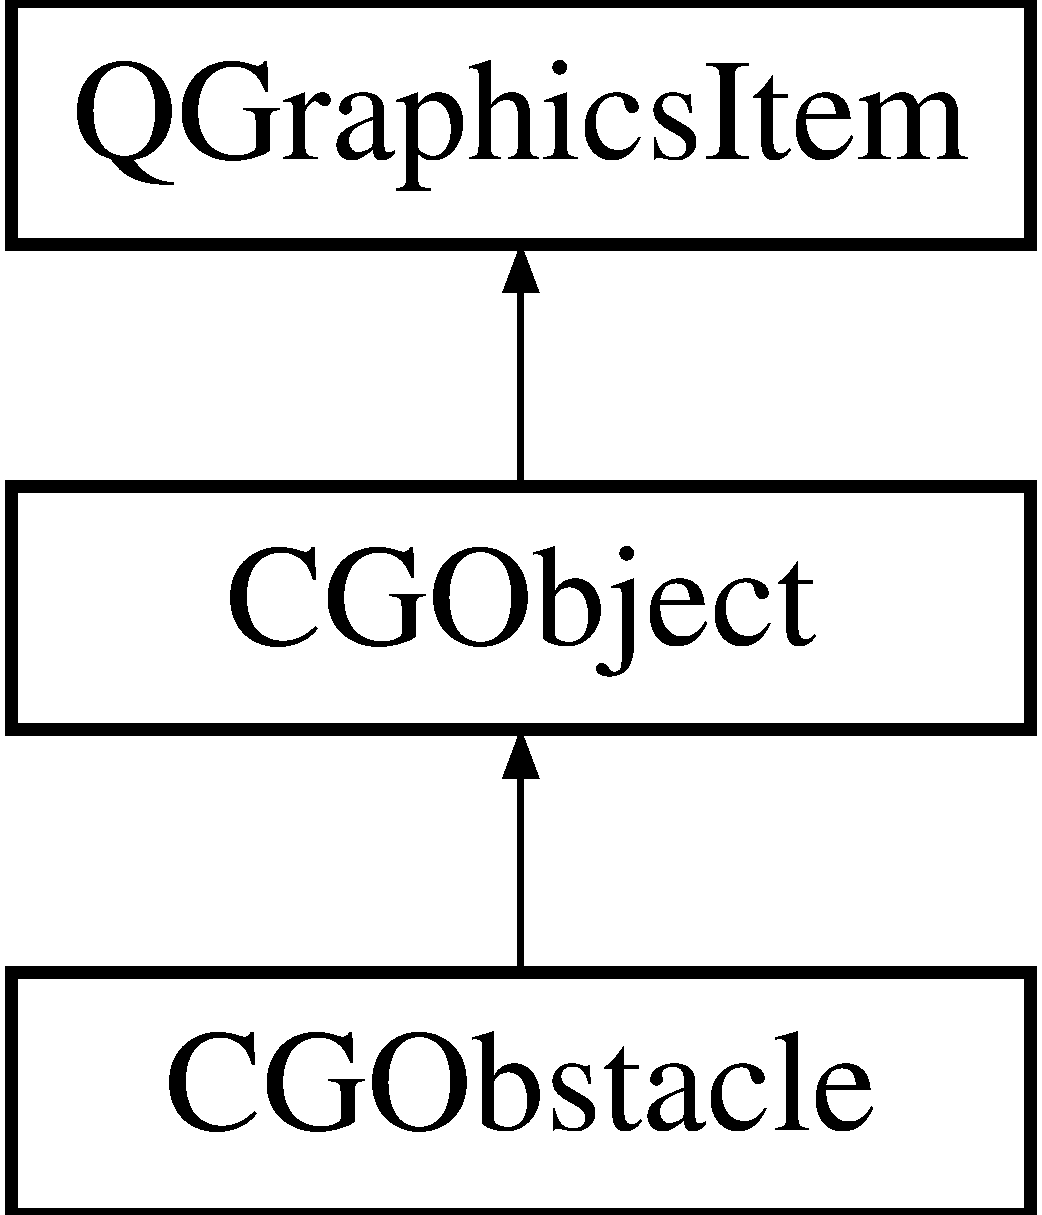
\includegraphics[height=3.000000cm]{class_c_g_obstacle}
\end{center}
\end{figure}
\subsection*{Public Member Functions}
\begin{DoxyCompactItemize}
\item 
\mbox{\hyperlink{class_c_g_obstacle_af085e19a335a0e9c232f3b6766af79cd}{C\+G\+Obstacle}} (\mbox{\hyperlink{class_c_object}{C\+Object}} $\ast$o)
\item 
void \mbox{\hyperlink{class_c_g_obstacle_a4ae41138f5fa9f7929c71f1999df7793}{paint}} (Q\+Painter $\ast$painter, const Q\+Style\+Option\+Graphics\+Item $\ast$option, Q\+Widget $\ast$widget) override
\begin{DoxyCompactList}\small\item\em Funkcja określająca kształt obiektu, jej implementacja zależy od rodzaju klasy pochodnej. \end{DoxyCompactList}\item 
Q\+RectF \mbox{\hyperlink{class_c_g_obstacle_a88a124737ae6f96c6b07316591ecdb34}{bounding\+Rect}} () const override
\begin{DoxyCompactList}\small\item\em Zwraca prostokąt reprezentujący obrys obiektu; potrzebne do prawidłowego odświeżania obiektu na mapie; implementacja różna dla klas pochodnych. \end{DoxyCompactList}\item 
void \mbox{\hyperlink{class_c_g_obstacle_adeb38e94e73f2c3d5d84afbb5e5e0fe7}{advance}} () override
\begin{DoxyCompactList}\small\item\em Funkcja rysująca obiekt na mapie na podstawie parametrów obiektu logicznego. \end{DoxyCompactList}\item 
Q\+Painter\+Path \mbox{\hyperlink{class_c_g_obstacle_a850f592630a96855bc6fb7b8e4eece40}{shape}} () const override
\end{DoxyCompactItemize}
\subsection*{Additional Inherited Members}


\subsection{Detailed Description}
Graficzna reprezentacja przeszkody. 

\subsection{Constructor \& Destructor Documentation}
\mbox{\Hypertarget{class_c_g_obstacle_af085e19a335a0e9c232f3b6766af79cd}\label{class_c_g_obstacle_af085e19a335a0e9c232f3b6766af79cd}} 
\index{C\+G\+Obstacle@{C\+G\+Obstacle}!C\+G\+Obstacle@{C\+G\+Obstacle}}
\index{C\+G\+Obstacle@{C\+G\+Obstacle}!C\+G\+Obstacle@{C\+G\+Obstacle}}
\subsubsection{\texorpdfstring{C\+G\+Obstacle()}{CGObstacle()}}
{\footnotesize\ttfamily C\+G\+Obstacle\+::\+C\+G\+Obstacle (\begin{DoxyParamCaption}\item[{\mbox{\hyperlink{class_c_object}{C\+Object}} $\ast$}]{o }\end{DoxyParamCaption})}



\subsection{Member Function Documentation}
\mbox{\Hypertarget{class_c_g_obstacle_adeb38e94e73f2c3d5d84afbb5e5e0fe7}\label{class_c_g_obstacle_adeb38e94e73f2c3d5d84afbb5e5e0fe7}} 
\index{C\+G\+Obstacle@{C\+G\+Obstacle}!advance@{advance}}
\index{advance@{advance}!C\+G\+Obstacle@{C\+G\+Obstacle}}
\subsubsection{\texorpdfstring{advance()}{advance()}}
{\footnotesize\ttfamily void C\+G\+Obstacle\+::advance (\begin{DoxyParamCaption}{ }\end{DoxyParamCaption})\hspace{0.3cm}{\ttfamily [override]}, {\ttfamily [virtual]}}



Funkcja rysująca obiekt na mapie na podstawie parametrów obiektu logicznego. 



Implements \mbox{\hyperlink{class_c_g_object_a859e765fbb3ab0d6ad73ca58e5e49779}{C\+G\+Object}}.

\mbox{\Hypertarget{class_c_g_obstacle_a88a124737ae6f96c6b07316591ecdb34}\label{class_c_g_obstacle_a88a124737ae6f96c6b07316591ecdb34}} 
\index{C\+G\+Obstacle@{C\+G\+Obstacle}!bounding\+Rect@{bounding\+Rect}}
\index{bounding\+Rect@{bounding\+Rect}!C\+G\+Obstacle@{C\+G\+Obstacle}}
\subsubsection{\texorpdfstring{bounding\+Rect()}{boundingRect()}}
{\footnotesize\ttfamily Q\+RectF C\+G\+Obstacle\+::bounding\+Rect (\begin{DoxyParamCaption}{ }\end{DoxyParamCaption}) const\hspace{0.3cm}{\ttfamily [override]}, {\ttfamily [virtual]}}



Zwraca prostokąt reprezentujący obrys obiektu; potrzebne do prawidłowego odświeżania obiektu na mapie; implementacja różna dla klas pochodnych. 

\begin{DoxyReturn}{Returns}
Q\+RecF reprezentujący obrys obiektu 
\end{DoxyReturn}


Implements \mbox{\hyperlink{class_c_g_object_ab9edf3d10a53c254cdb5d3d8de930207}{C\+G\+Object}}.

\mbox{\Hypertarget{class_c_g_obstacle_a4ae41138f5fa9f7929c71f1999df7793}\label{class_c_g_obstacle_a4ae41138f5fa9f7929c71f1999df7793}} 
\index{C\+G\+Obstacle@{C\+G\+Obstacle}!paint@{paint}}
\index{paint@{paint}!C\+G\+Obstacle@{C\+G\+Obstacle}}
\subsubsection{\texorpdfstring{paint()}{paint()}}
{\footnotesize\ttfamily void C\+G\+Obstacle\+::paint (\begin{DoxyParamCaption}\item[{Q\+Painter $\ast$}]{painter,  }\item[{const Q\+Style\+Option\+Graphics\+Item $\ast$}]{option,  }\item[{Q\+Widget $\ast$}]{widget }\end{DoxyParamCaption})\hspace{0.3cm}{\ttfamily [override]}, {\ttfamily [virtual]}}



Funkcja określająca kształt obiektu, jej implementacja zależy od rodzaju klasy pochodnej. 


\begin{DoxyParams}{Parameters}
{\em painter} & \\
\hline
{\em option} & \\
\hline
{\em widget} & \\
\hline
\end{DoxyParams}


Implements \mbox{\hyperlink{class_c_g_object_a9622c313eb09ca5fc0e34f5d2aaac910}{C\+G\+Object}}.

\mbox{\Hypertarget{class_c_g_obstacle_a850f592630a96855bc6fb7b8e4eece40}\label{class_c_g_obstacle_a850f592630a96855bc6fb7b8e4eece40}} 
\index{C\+G\+Obstacle@{C\+G\+Obstacle}!shape@{shape}}
\index{shape@{shape}!C\+G\+Obstacle@{C\+G\+Obstacle}}
\subsubsection{\texorpdfstring{shape()}{shape()}}
{\footnotesize\ttfamily Q\+Painter\+Path C\+G\+Obstacle\+::shape (\begin{DoxyParamCaption}{ }\end{DoxyParamCaption}) const\hspace{0.3cm}{\ttfamily [override]}}



The documentation for this class was generated from the following files\+:\begin{DoxyCompactItemize}
\item 
\mbox{\hyperlink{cgobstacle_8h}{cgobstacle.\+h}}\item 
\mbox{\hyperlink{cgobstacle_8cpp}{cgobstacle.\+cpp}}\end{DoxyCompactItemize}

\hypertarget{class_c_g_searching_robot}{}\section{C\+G\+Searching\+Robot Class Reference}
\label{class_c_g_searching_robot}\index{C\+G\+Searching\+Robot@{C\+G\+Searching\+Robot}}


Graficzna reprezentacja robota szukającego.  




{\ttfamily \#include $<$cgsearchingrobot.\+h$>$}

Inheritance diagram for C\+G\+Searching\+Robot\+:\begin{figure}[H]
\begin{center}
\leavevmode
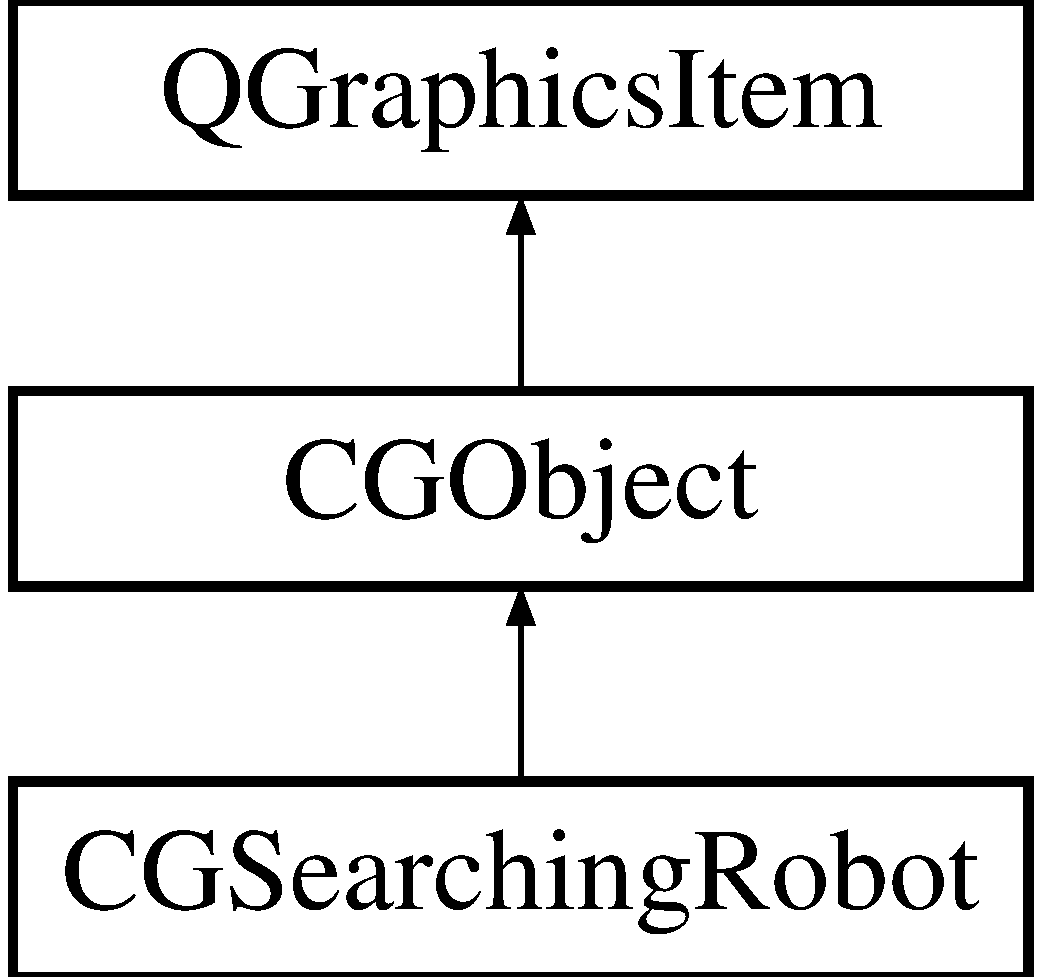
\includegraphics[height=3.000000cm]{class_c_g_searching_robot}
\end{center}
\end{figure}
\subsection*{Public Member Functions}
\begin{DoxyCompactItemize}
\item 
\mbox{\hyperlink{class_c_g_searching_robot_a6d8b0f84b870aa6af83323d72d0bf010}{C\+G\+Searching\+Robot}} (\mbox{\hyperlink{class_c_object}{C\+Object}} $\ast$o)
\item 
void \mbox{\hyperlink{class_c_g_searching_robot_ad6e9d94604256cb9f0fe6e708c4391ad}{paint}} (Q\+Painter $\ast$painter, const Q\+Style\+Option\+Graphics\+Item $\ast$option, Q\+Widget $\ast$widget) override
\begin{DoxyCompactList}\small\item\em Funkcja określająca kształt obiektu, jej implementacja zależy od rodzaju klasy pochodnej. \end{DoxyCompactList}\item 
Q\+RectF \mbox{\hyperlink{class_c_g_searching_robot_aa0cf51f6acdfa865c130f0cd16860625}{bounding\+Rect}} () const override
\begin{DoxyCompactList}\small\item\em Zwraca prostokąt reprezentujący obrys obiektu; potrzebne do prawidłowego odświeżania obiektu na mapie; implementacja różna dla klas pochodnych. \end{DoxyCompactList}\item 
void \mbox{\hyperlink{class_c_g_searching_robot_adcc4b3096e11c25287806428119acb22}{advance}} () override
\begin{DoxyCompactList}\small\item\em Funkcja rysująca obiekt na mapie na podstawie parametrów obiektu logicznego. \end{DoxyCompactList}\item 
Q\+Painter\+Path \mbox{\hyperlink{class_c_g_searching_robot_acd63b054e31c88aaf2070a829e1f897a}{shape}} () const override
\end{DoxyCompactItemize}
\subsection*{Additional Inherited Members}


\subsection{Detailed Description}
Graficzna reprezentacja robota szukającego. 

\subsection{Constructor \& Destructor Documentation}
\mbox{\Hypertarget{class_c_g_searching_robot_a6d8b0f84b870aa6af83323d72d0bf010}\label{class_c_g_searching_robot_a6d8b0f84b870aa6af83323d72d0bf010}} 
\index{C\+G\+Searching\+Robot@{C\+G\+Searching\+Robot}!C\+G\+Searching\+Robot@{C\+G\+Searching\+Robot}}
\index{C\+G\+Searching\+Robot@{C\+G\+Searching\+Robot}!C\+G\+Searching\+Robot@{C\+G\+Searching\+Robot}}
\subsubsection{\texorpdfstring{C\+G\+Searching\+Robot()}{CGSearchingRobot()}}
{\footnotesize\ttfamily C\+G\+Searching\+Robot\+::\+C\+G\+Searching\+Robot (\begin{DoxyParamCaption}\item[{\mbox{\hyperlink{class_c_object}{C\+Object}} $\ast$}]{o }\end{DoxyParamCaption})}



\subsection{Member Function Documentation}
\mbox{\Hypertarget{class_c_g_searching_robot_adcc4b3096e11c25287806428119acb22}\label{class_c_g_searching_robot_adcc4b3096e11c25287806428119acb22}} 
\index{C\+G\+Searching\+Robot@{C\+G\+Searching\+Robot}!advance@{advance}}
\index{advance@{advance}!C\+G\+Searching\+Robot@{C\+G\+Searching\+Robot}}
\subsubsection{\texorpdfstring{advance()}{advance()}}
{\footnotesize\ttfamily void C\+G\+Searching\+Robot\+::advance (\begin{DoxyParamCaption}{ }\end{DoxyParamCaption})\hspace{0.3cm}{\ttfamily [override]}, {\ttfamily [virtual]}}



Funkcja rysująca obiekt na mapie na podstawie parametrów obiektu logicznego. 



Implements \mbox{\hyperlink{class_c_g_object_a859e765fbb3ab0d6ad73ca58e5e49779}{C\+G\+Object}}.

\mbox{\Hypertarget{class_c_g_searching_robot_aa0cf51f6acdfa865c130f0cd16860625}\label{class_c_g_searching_robot_aa0cf51f6acdfa865c130f0cd16860625}} 
\index{C\+G\+Searching\+Robot@{C\+G\+Searching\+Robot}!bounding\+Rect@{bounding\+Rect}}
\index{bounding\+Rect@{bounding\+Rect}!C\+G\+Searching\+Robot@{C\+G\+Searching\+Robot}}
\subsubsection{\texorpdfstring{bounding\+Rect()}{boundingRect()}}
{\footnotesize\ttfamily Q\+RectF C\+G\+Searching\+Robot\+::bounding\+Rect (\begin{DoxyParamCaption}{ }\end{DoxyParamCaption}) const\hspace{0.3cm}{\ttfamily [override]}, {\ttfamily [virtual]}}



Zwraca prostokąt reprezentujący obrys obiektu; potrzebne do prawidłowego odświeżania obiektu na mapie; implementacja różna dla klas pochodnych. 

\begin{DoxyReturn}{Returns}
Q\+RecF reprezentujący obrys obiektu 
\end{DoxyReturn}


Implements \mbox{\hyperlink{class_c_g_object_ab9edf3d10a53c254cdb5d3d8de930207}{C\+G\+Object}}.

\mbox{\Hypertarget{class_c_g_searching_robot_ad6e9d94604256cb9f0fe6e708c4391ad}\label{class_c_g_searching_robot_ad6e9d94604256cb9f0fe6e708c4391ad}} 
\index{C\+G\+Searching\+Robot@{C\+G\+Searching\+Robot}!paint@{paint}}
\index{paint@{paint}!C\+G\+Searching\+Robot@{C\+G\+Searching\+Robot}}
\subsubsection{\texorpdfstring{paint()}{paint()}}
{\footnotesize\ttfamily void C\+G\+Searching\+Robot\+::paint (\begin{DoxyParamCaption}\item[{Q\+Painter $\ast$}]{painter,  }\item[{const Q\+Style\+Option\+Graphics\+Item $\ast$}]{option,  }\item[{Q\+Widget $\ast$}]{widget }\end{DoxyParamCaption})\hspace{0.3cm}{\ttfamily [override]}, {\ttfamily [virtual]}}



Funkcja określająca kształt obiektu, jej implementacja zależy od rodzaju klasy pochodnej. 


\begin{DoxyParams}{Parameters}
{\em painter} & \\
\hline
{\em option} & \\
\hline
{\em widget} & \\
\hline
\end{DoxyParams}


Implements \mbox{\hyperlink{class_c_g_object_a9622c313eb09ca5fc0e34f5d2aaac910}{C\+G\+Object}}.

\mbox{\Hypertarget{class_c_g_searching_robot_acd63b054e31c88aaf2070a829e1f897a}\label{class_c_g_searching_robot_acd63b054e31c88aaf2070a829e1f897a}} 
\index{C\+G\+Searching\+Robot@{C\+G\+Searching\+Robot}!shape@{shape}}
\index{shape@{shape}!C\+G\+Searching\+Robot@{C\+G\+Searching\+Robot}}
\subsubsection{\texorpdfstring{shape()}{shape()}}
{\footnotesize\ttfamily Q\+Painter\+Path C\+G\+Searching\+Robot\+::shape (\begin{DoxyParamCaption}{ }\end{DoxyParamCaption}) const\hspace{0.3cm}{\ttfamily [override]}}



The documentation for this class was generated from the following files\+:\begin{DoxyCompactItemize}
\item 
\mbox{\hyperlink{cgsearchingrobot_8h}{cgsearchingrobot.\+h}}\item 
\mbox{\hyperlink{cgsearchingrobot_8cpp}{cgsearchingrobot.\+cpp}}\end{DoxyCompactItemize}

\hypertarget{class_c_g_treasure}{}\section{C\+G\+Treasure Class Reference}
\label{class_c_g_treasure}\index{C\+G\+Treasure@{C\+G\+Treasure}}


Graficzna reprezentacja skarbu.  




{\ttfamily \#include $<$cgtreasure.\+h$>$}

Inheritance diagram for C\+G\+Treasure\+:\begin{figure}[H]
\begin{center}
\leavevmode
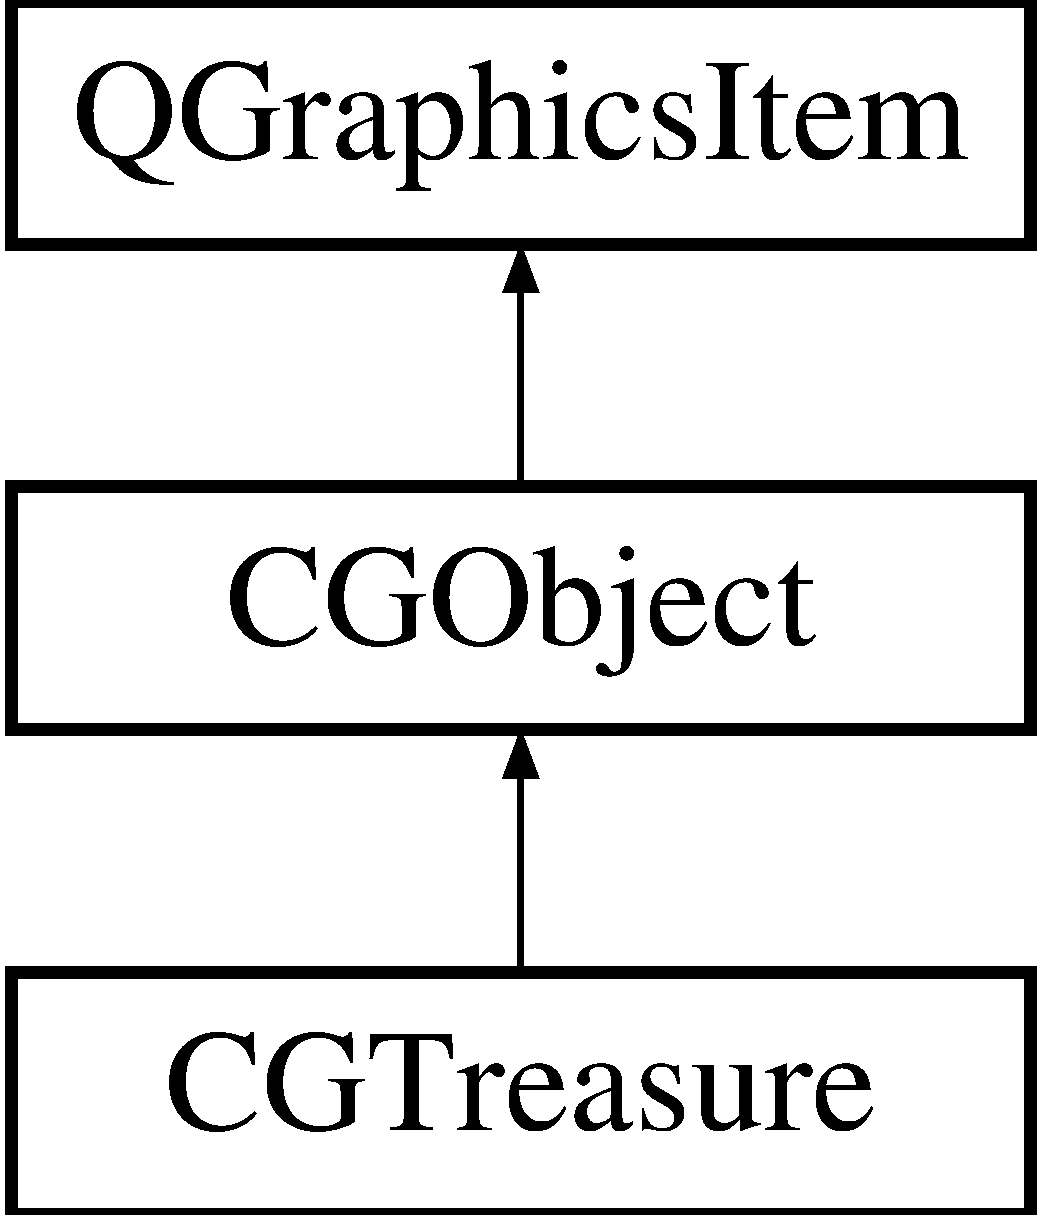
\includegraphics[height=3.000000cm]{class_c_g_treasure}
\end{center}
\end{figure}
\subsection*{Public Member Functions}
\begin{DoxyCompactItemize}
\item 
\mbox{\hyperlink{class_c_g_treasure_a325defc3d5c7f5648d7c8d339a0be527}{C\+G\+Treasure}} (\mbox{\hyperlink{class_c_object}{C\+Object}} $\ast$o)
\item 
void \mbox{\hyperlink{class_c_g_treasure_aeab69a95590acb46aa4d20422be96560}{paint}} (Q\+Painter $\ast$painter, const Q\+Style\+Option\+Graphics\+Item $\ast$option, Q\+Widget $\ast$widget) override
\begin{DoxyCompactList}\small\item\em Funkcja określająca kształt obiektu, jej implementacja zależy od rodzaju klasy pochodnej. \end{DoxyCompactList}\item 
Q\+RectF \mbox{\hyperlink{class_c_g_treasure_a103be7d49202d07d9260917a7d6e8429}{bounding\+Rect}} () const override
\begin{DoxyCompactList}\small\item\em Zwraca prostokąt reprezentujący obrys obiektu; potrzebne do prawidłowego odświeżania obiektu na mapie; implementacja różna dla klas pochodnych. \end{DoxyCompactList}\item 
void \mbox{\hyperlink{class_c_g_treasure_a4b8a13bcae320e63a87a32a804606190}{advance}} () override
\begin{DoxyCompactList}\small\item\em Funkcja rysująca obiekt na mapie na podstawie parametrów obiektu logicznego. \end{DoxyCompactList}\item 
Q\+Painter\+Path \mbox{\hyperlink{class_c_g_treasure_a021ffe6c72146aa0e3789cf9d111ccb2}{shape}} () const override
\end{DoxyCompactItemize}
\subsection*{Additional Inherited Members}


\subsection{Detailed Description}
Graficzna reprezentacja skarbu. 

\subsection{Constructor \& Destructor Documentation}
\mbox{\Hypertarget{class_c_g_treasure_a325defc3d5c7f5648d7c8d339a0be527}\label{class_c_g_treasure_a325defc3d5c7f5648d7c8d339a0be527}} 
\index{C\+G\+Treasure@{C\+G\+Treasure}!C\+G\+Treasure@{C\+G\+Treasure}}
\index{C\+G\+Treasure@{C\+G\+Treasure}!C\+G\+Treasure@{C\+G\+Treasure}}
\subsubsection{\texorpdfstring{C\+G\+Treasure()}{CGTreasure()}}
{\footnotesize\ttfamily C\+G\+Treasure\+::\+C\+G\+Treasure (\begin{DoxyParamCaption}\item[{\mbox{\hyperlink{class_c_object}{C\+Object}} $\ast$}]{o }\end{DoxyParamCaption})}



\subsection{Member Function Documentation}
\mbox{\Hypertarget{class_c_g_treasure_a4b8a13bcae320e63a87a32a804606190}\label{class_c_g_treasure_a4b8a13bcae320e63a87a32a804606190}} 
\index{C\+G\+Treasure@{C\+G\+Treasure}!advance@{advance}}
\index{advance@{advance}!C\+G\+Treasure@{C\+G\+Treasure}}
\subsubsection{\texorpdfstring{advance()}{advance()}}
{\footnotesize\ttfamily void C\+G\+Treasure\+::advance (\begin{DoxyParamCaption}{ }\end{DoxyParamCaption})\hspace{0.3cm}{\ttfamily [override]}, {\ttfamily [virtual]}}



Funkcja rysująca obiekt na mapie na podstawie parametrów obiektu logicznego. 



Implements \mbox{\hyperlink{class_c_g_object_a859e765fbb3ab0d6ad73ca58e5e49779}{C\+G\+Object}}.

\mbox{\Hypertarget{class_c_g_treasure_a103be7d49202d07d9260917a7d6e8429}\label{class_c_g_treasure_a103be7d49202d07d9260917a7d6e8429}} 
\index{C\+G\+Treasure@{C\+G\+Treasure}!bounding\+Rect@{bounding\+Rect}}
\index{bounding\+Rect@{bounding\+Rect}!C\+G\+Treasure@{C\+G\+Treasure}}
\subsubsection{\texorpdfstring{bounding\+Rect()}{boundingRect()}}
{\footnotesize\ttfamily Q\+RectF C\+G\+Treasure\+::bounding\+Rect (\begin{DoxyParamCaption}{ }\end{DoxyParamCaption}) const\hspace{0.3cm}{\ttfamily [override]}, {\ttfamily [virtual]}}



Zwraca prostokąt reprezentujący obrys obiektu; potrzebne do prawidłowego odświeżania obiektu na mapie; implementacja różna dla klas pochodnych. 

\begin{DoxyReturn}{Returns}
Q\+RecF reprezentujący obrys obiektu 
\end{DoxyReturn}


Implements \mbox{\hyperlink{class_c_g_object_ab9edf3d10a53c254cdb5d3d8de930207}{C\+G\+Object}}.

\mbox{\Hypertarget{class_c_g_treasure_aeab69a95590acb46aa4d20422be96560}\label{class_c_g_treasure_aeab69a95590acb46aa4d20422be96560}} 
\index{C\+G\+Treasure@{C\+G\+Treasure}!paint@{paint}}
\index{paint@{paint}!C\+G\+Treasure@{C\+G\+Treasure}}
\subsubsection{\texorpdfstring{paint()}{paint()}}
{\footnotesize\ttfamily void C\+G\+Treasure\+::paint (\begin{DoxyParamCaption}\item[{Q\+Painter $\ast$}]{painter,  }\item[{const Q\+Style\+Option\+Graphics\+Item $\ast$}]{option,  }\item[{Q\+Widget $\ast$}]{widget }\end{DoxyParamCaption})\hspace{0.3cm}{\ttfamily [override]}, {\ttfamily [virtual]}}



Funkcja określająca kształt obiektu, jej implementacja zależy od rodzaju klasy pochodnej. 


\begin{DoxyParams}{Parameters}
{\em painter} & \\
\hline
{\em option} & \\
\hline
{\em widget} & \\
\hline
\end{DoxyParams}


Implements \mbox{\hyperlink{class_c_g_object_a9622c313eb09ca5fc0e34f5d2aaac910}{C\+G\+Object}}.

\mbox{\Hypertarget{class_c_g_treasure_a021ffe6c72146aa0e3789cf9d111ccb2}\label{class_c_g_treasure_a021ffe6c72146aa0e3789cf9d111ccb2}} 
\index{C\+G\+Treasure@{C\+G\+Treasure}!shape@{shape}}
\index{shape@{shape}!C\+G\+Treasure@{C\+G\+Treasure}}
\subsubsection{\texorpdfstring{shape()}{shape()}}
{\footnotesize\ttfamily Q\+Painter\+Path C\+G\+Treasure\+::shape (\begin{DoxyParamCaption}{ }\end{DoxyParamCaption}) const\hspace{0.3cm}{\ttfamily [override]}}



The documentation for this class was generated from the following files\+:\begin{DoxyCompactItemize}
\item 
\mbox{\hyperlink{cgtreasure_8h}{cgtreasure.\+h}}\item 
\mbox{\hyperlink{cgtreasure_8cpp}{cgtreasure.\+cpp}}\end{DoxyCompactItemize}

\hypertarget{class_c_map}{}\section{C\+Map Class Reference}
\label{class_c_map}\index{C\+Map@{C\+Map}}


Mapa, na której poruszają się wszystkie obiekty.  




{\ttfamily \#include $<$cmap.\+h$>$}

\subsection*{Public Member Functions}
\begin{DoxyCompactItemize}
\item 
\mbox{\hyperlink{class_c_map_a23632998cdecdd0b9c77c799e5d5d51b}{C\+Map}} (Q\+Graphics\+Scene $\ast$scene)
\begin{DoxyCompactList}\small\item\em Konstruktor wymaga podania wskaźnika do sceny oraz tworzy określoną ilość obiektów różnego typu na mapie. \end{DoxyCompactList}\item 
Q\+Graphics\+Scene $\ast$ \mbox{\hyperlink{class_c_map_ac2282caabd7d3830bd1c731177883e50}{get\+Scene}} ()
\begin{DoxyCompactList}\small\item\em Funkcja zwracająca wskaźnik do sceny. \end{DoxyCompactList}\item 
std\+::vector$<$ \mbox{\hyperlink{class_c_object}{C\+Object}} $\ast$ $>$ \mbox{\hyperlink{class_c_map_ae6b5f2e5ca9db035092b730ad92a4aaf}{get\+Object\+List}} ()
\begin{DoxyCompactList}\small\item\em Funkcja zwracająca wskaźnik na wszystkie obiekty logiczne przypisane do mapy. \end{DoxyCompactList}\item 
std\+::vector$<$ \mbox{\hyperlink{class_c_g_object}{C\+G\+Object}} $\ast$ $>$ \mbox{\hyperlink{class_c_map_ab37b3b5bf85c57a891ed2fd591a01ea9}{get\+G\+Object\+List}} ()
\begin{DoxyCompactList}\small\item\em Funkcja zwracająca wskaźnik na wszystkie obiekty graficzne przypisane do mapy. \end{DoxyCompactList}\item 
std\+::vector$<$ \mbox{\hyperlink{class_c_object}{C\+Object}} $\ast$ $>$ \mbox{\hyperlink{class_c_map_aee9422cd38e050f52fb42bf2e7f4e8ed}{get\+Neighboors\+List}} (\mbox{\hyperlink{class_c_object}{C\+Object}} $\ast$o)
\begin{DoxyCompactList}\small\item\em Funkcja zwracająca wektor innych obiektów znajdujących się w zasięgu wskazanego obiektu. \end{DoxyCompactList}\item 
void \mbox{\hyperlink{class_c_map_a4b22b964e9d16e428c0a56b15b235c82}{add\+Object}} (\mbox{\hyperlink{class_c_object}{C\+Object}} $\ast$object)
\begin{DoxyCompactList}\small\item\em Dodaje wskazany obiekt logiczny do listy obiektów znajdujących się na mapie. \end{DoxyCompactList}\item 
void \mbox{\hyperlink{class_c_map_adfb0980e5f2153cd6b287a010795c6b4}{add\+G\+Object}} (\mbox{\hyperlink{class_c_g_object}{C\+G\+Object}} $\ast$gobject)
\begin{DoxyCompactList}\small\item\em Dodaje wskazany obiekt graficzny do listy obiektów znajdujących się na mapie. \end{DoxyCompactList}\item 
void \mbox{\hyperlink{class_c_map_a55bccb7dd240a21de6e5d12df054d0cb}{delete\+From\+Map}} (\mbox{\hyperlink{class_c_object}{C\+Object}} $\ast$o)
\begin{DoxyCompactList}\small\item\em Usuwa z listy obiektów na mapie obiekt graficzny oraz odpowiadający mu obiekt logiczny. \end{DoxyCompactList}\item 
{\footnotesize template$<$class object\+\_\+type , class gobject\+\_\+type $>$ }\\void \mbox{\hyperlink{class_c_map_a448bdffc8a0a0fcbd39e1e7661b5d6ab}{add}} (int n)
\begin{DoxyCompactList}\small\item\em Szablon służący do tworzenia na mapie nowych obiektów o podanym typie param n Ilość obiektów danego typu, które chcemy utworzyć \end{DoxyCompactList}\item 
{\footnotesize template$<$class object\+\_\+type , class gobject\+\_\+type $>$ }\\void \mbox{\hyperlink{class_c_map_a194d39490529731472920eac44df1548}{spawn}} (int x)
\begin{DoxyCompactList}\small\item\em Szablon służący do tworzenia obiektu danego typu z prawdopodobieństwem 1/x, wywoływany przy każdym kroku programu param x Określa prawdopodobieństwo, z jakim dodany zostanie obiekt. \end{DoxyCompactList}\end{DoxyCompactItemize}


\subsection{Detailed Description}
Mapa, na której poruszają się wszystkie obiekty. 

\subsection{Constructor \& Destructor Documentation}
\mbox{\Hypertarget{class_c_map_a23632998cdecdd0b9c77c799e5d5d51b}\label{class_c_map_a23632998cdecdd0b9c77c799e5d5d51b}} 
\index{C\+Map@{C\+Map}!C\+Map@{C\+Map}}
\index{C\+Map@{C\+Map}!C\+Map@{C\+Map}}
\subsubsection{\texorpdfstring{C\+Map()}{CMap()}}
{\footnotesize\ttfamily C\+Map\+::\+C\+Map (\begin{DoxyParamCaption}\item[{Q\+Graphics\+Scene $\ast$}]{scene }\end{DoxyParamCaption})}



Konstruktor wymaga podania wskaźnika do sceny oraz tworzy określoną ilość obiektów różnego typu na mapie. 


\begin{DoxyParams}{Parameters}
{\em scene} & Scena, na której umieszczone zostaną wszystkie obiekty \\
\hline
\end{DoxyParams}


\subsection{Member Function Documentation}
\mbox{\Hypertarget{class_c_map_a448bdffc8a0a0fcbd39e1e7661b5d6ab}\label{class_c_map_a448bdffc8a0a0fcbd39e1e7661b5d6ab}} 
\index{C\+Map@{C\+Map}!add@{add}}
\index{add@{add}!C\+Map@{C\+Map}}
\subsubsection{\texorpdfstring{add()}{add()}}
{\footnotesize\ttfamily template$<$class object\+\_\+type , class gobject\+\_\+type $>$ \\
void C\+Map\+::add (\begin{DoxyParamCaption}\item[{int}]{n }\end{DoxyParamCaption})\hspace{0.3cm}{\ttfamily [inline]}}



Szablon służący do tworzenia na mapie nowych obiektów o podanym typie param n Ilość obiektów danego typu, które chcemy utworzyć 

\mbox{\Hypertarget{class_c_map_adfb0980e5f2153cd6b287a010795c6b4}\label{class_c_map_adfb0980e5f2153cd6b287a010795c6b4}} 
\index{C\+Map@{C\+Map}!add\+G\+Object@{add\+G\+Object}}
\index{add\+G\+Object@{add\+G\+Object}!C\+Map@{C\+Map}}
\subsubsection{\texorpdfstring{add\+G\+Object()}{addGObject()}}
{\footnotesize\ttfamily void C\+Map\+::add\+G\+Object (\begin{DoxyParamCaption}\item[{\mbox{\hyperlink{class_c_g_object}{C\+G\+Object}} $\ast$}]{gobject }\end{DoxyParamCaption})}



Dodaje wskazany obiekt graficzny do listy obiektów znajdujących się na mapie. 


\begin{DoxyParams}{Parameters}
{\em gobject} & Obiekt, który należy dodać do mapy \\
\hline
\end{DoxyParams}
\mbox{\Hypertarget{class_c_map_a4b22b964e9d16e428c0a56b15b235c82}\label{class_c_map_a4b22b964e9d16e428c0a56b15b235c82}} 
\index{C\+Map@{C\+Map}!add\+Object@{add\+Object}}
\index{add\+Object@{add\+Object}!C\+Map@{C\+Map}}
\subsubsection{\texorpdfstring{add\+Object()}{addObject()}}
{\footnotesize\ttfamily void C\+Map\+::add\+Object (\begin{DoxyParamCaption}\item[{\mbox{\hyperlink{class_c_object}{C\+Object}} $\ast$}]{object }\end{DoxyParamCaption})}



Dodaje wskazany obiekt logiczny do listy obiektów znajdujących się na mapie. 


\begin{DoxyParams}{Parameters}
{\em object} & Obiekt, który należy dodać do mapy \\
\hline
\end{DoxyParams}
\mbox{\Hypertarget{class_c_map_a55bccb7dd240a21de6e5d12df054d0cb}\label{class_c_map_a55bccb7dd240a21de6e5d12df054d0cb}} 
\index{C\+Map@{C\+Map}!delete\+From\+Map@{delete\+From\+Map}}
\index{delete\+From\+Map@{delete\+From\+Map}!C\+Map@{C\+Map}}
\subsubsection{\texorpdfstring{delete\+From\+Map()}{deleteFromMap()}}
{\footnotesize\ttfamily void C\+Map\+::delete\+From\+Map (\begin{DoxyParamCaption}\item[{\mbox{\hyperlink{class_c_object}{C\+Object}} $\ast$}]{o }\end{DoxyParamCaption})}



Usuwa z listy obiektów na mapie obiekt graficzny oraz odpowiadający mu obiekt logiczny. 


\begin{DoxyParams}{Parameters}
{\em o} & Obiekt, który chcemy usunąc z mapy \\
\hline
\end{DoxyParams}
\mbox{\Hypertarget{class_c_map_ab37b3b5bf85c57a891ed2fd591a01ea9}\label{class_c_map_ab37b3b5bf85c57a891ed2fd591a01ea9}} 
\index{C\+Map@{C\+Map}!get\+G\+Object\+List@{get\+G\+Object\+List}}
\index{get\+G\+Object\+List@{get\+G\+Object\+List}!C\+Map@{C\+Map}}
\subsubsection{\texorpdfstring{get\+G\+Object\+List()}{getGObjectList()}}
{\footnotesize\ttfamily std\+::vector$<$ \mbox{\hyperlink{class_c_g_object}{C\+G\+Object}} $\ast$ $>$ C\+Map\+::get\+G\+Object\+List (\begin{DoxyParamCaption}{ }\end{DoxyParamCaption})}



Funkcja zwracająca wskaźnik na wszystkie obiekty graficzne przypisane do mapy. 

\begin{DoxyReturn}{Returns}
G\+Object\+List 
\end{DoxyReturn}
\mbox{\Hypertarget{class_c_map_aee9422cd38e050f52fb42bf2e7f4e8ed}\label{class_c_map_aee9422cd38e050f52fb42bf2e7f4e8ed}} 
\index{C\+Map@{C\+Map}!get\+Neighboors\+List@{get\+Neighboors\+List}}
\index{get\+Neighboors\+List@{get\+Neighboors\+List}!C\+Map@{C\+Map}}
\subsubsection{\texorpdfstring{get\+Neighboors\+List()}{getNeighboorsList()}}
{\footnotesize\ttfamily vector$<$ \mbox{\hyperlink{class_c_object}{C\+Object}} $\ast$ $>$ C\+Map\+::get\+Neighboors\+List (\begin{DoxyParamCaption}\item[{\mbox{\hyperlink{class_c_object}{C\+Object}} $\ast$}]{o }\end{DoxyParamCaption})}



Funkcja zwracająca wektor innych obiektów znajdujących się w zasięgu wskazanego obiektu. 


\begin{DoxyParams}{Parameters}
{\em o} & Obiekt, dla którego sprawdzane jest otoczenie \\
\hline
\end{DoxyParams}
\begin{DoxyReturn}{Returns}
Wektor obiektów, dla których odległość od o jest mniejsza od o.\+range 
\end{DoxyReturn}
\mbox{\Hypertarget{class_c_map_ae6b5f2e5ca9db035092b730ad92a4aaf}\label{class_c_map_ae6b5f2e5ca9db035092b730ad92a4aaf}} 
\index{C\+Map@{C\+Map}!get\+Object\+List@{get\+Object\+List}}
\index{get\+Object\+List@{get\+Object\+List}!C\+Map@{C\+Map}}
\subsubsection{\texorpdfstring{get\+Object\+List()}{getObjectList()}}
{\footnotesize\ttfamily std\+::vector$<$ \mbox{\hyperlink{class_c_object}{C\+Object}} $\ast$ $>$ C\+Map\+::get\+Object\+List (\begin{DoxyParamCaption}{ }\end{DoxyParamCaption})}



Funkcja zwracająca wskaźnik na wszystkie obiekty logiczne przypisane do mapy. 

\begin{DoxyReturn}{Returns}
Object\+List 
\end{DoxyReturn}
\mbox{\Hypertarget{class_c_map_ac2282caabd7d3830bd1c731177883e50}\label{class_c_map_ac2282caabd7d3830bd1c731177883e50}} 
\index{C\+Map@{C\+Map}!get\+Scene@{get\+Scene}}
\index{get\+Scene@{get\+Scene}!C\+Map@{C\+Map}}
\subsubsection{\texorpdfstring{get\+Scene()}{getScene()}}
{\footnotesize\ttfamily Q\+Graphics\+Scene $\ast$ C\+Map\+::get\+Scene (\begin{DoxyParamCaption}{ }\end{DoxyParamCaption})}



Funkcja zwracająca wskaźnik do sceny. 

\begin{DoxyReturn}{Returns}
scene 
\end{DoxyReturn}
\mbox{\Hypertarget{class_c_map_a194d39490529731472920eac44df1548}\label{class_c_map_a194d39490529731472920eac44df1548}} 
\index{C\+Map@{C\+Map}!spawn@{spawn}}
\index{spawn@{spawn}!C\+Map@{C\+Map}}
\subsubsection{\texorpdfstring{spawn()}{spawn()}}
{\footnotesize\ttfamily template$<$class object\+\_\+type , class gobject\+\_\+type $>$ \\
void C\+Map\+::spawn (\begin{DoxyParamCaption}\item[{int}]{x }\end{DoxyParamCaption})\hspace{0.3cm}{\ttfamily [inline]}}



Szablon służący do tworzenia obiektu danego typu z prawdopodobieństwem 1/x, wywoływany przy każdym kroku programu param x Określa prawdopodobieństwo, z jakim dodany zostanie obiekt. 



The documentation for this class was generated from the following files\+:\begin{DoxyCompactItemize}
\item 
\mbox{\hyperlink{cmap_8h}{cmap.\+h}}\item 
\mbox{\hyperlink{cmap_8cpp}{cmap.\+cpp}}\end{DoxyCompactItemize}

\hypertarget{class_c_mine}{}\section{C\+Mine Class Reference}
\label{class_c_mine}\index{C\+Mine@{C\+Mine}}


Mina niszcząca roboty, które na nią wpadną  




{\ttfamily \#include $<$cmine.\+h$>$}

Inheritance diagram for C\+Mine\+:\begin{figure}[H]
\begin{center}
\leavevmode
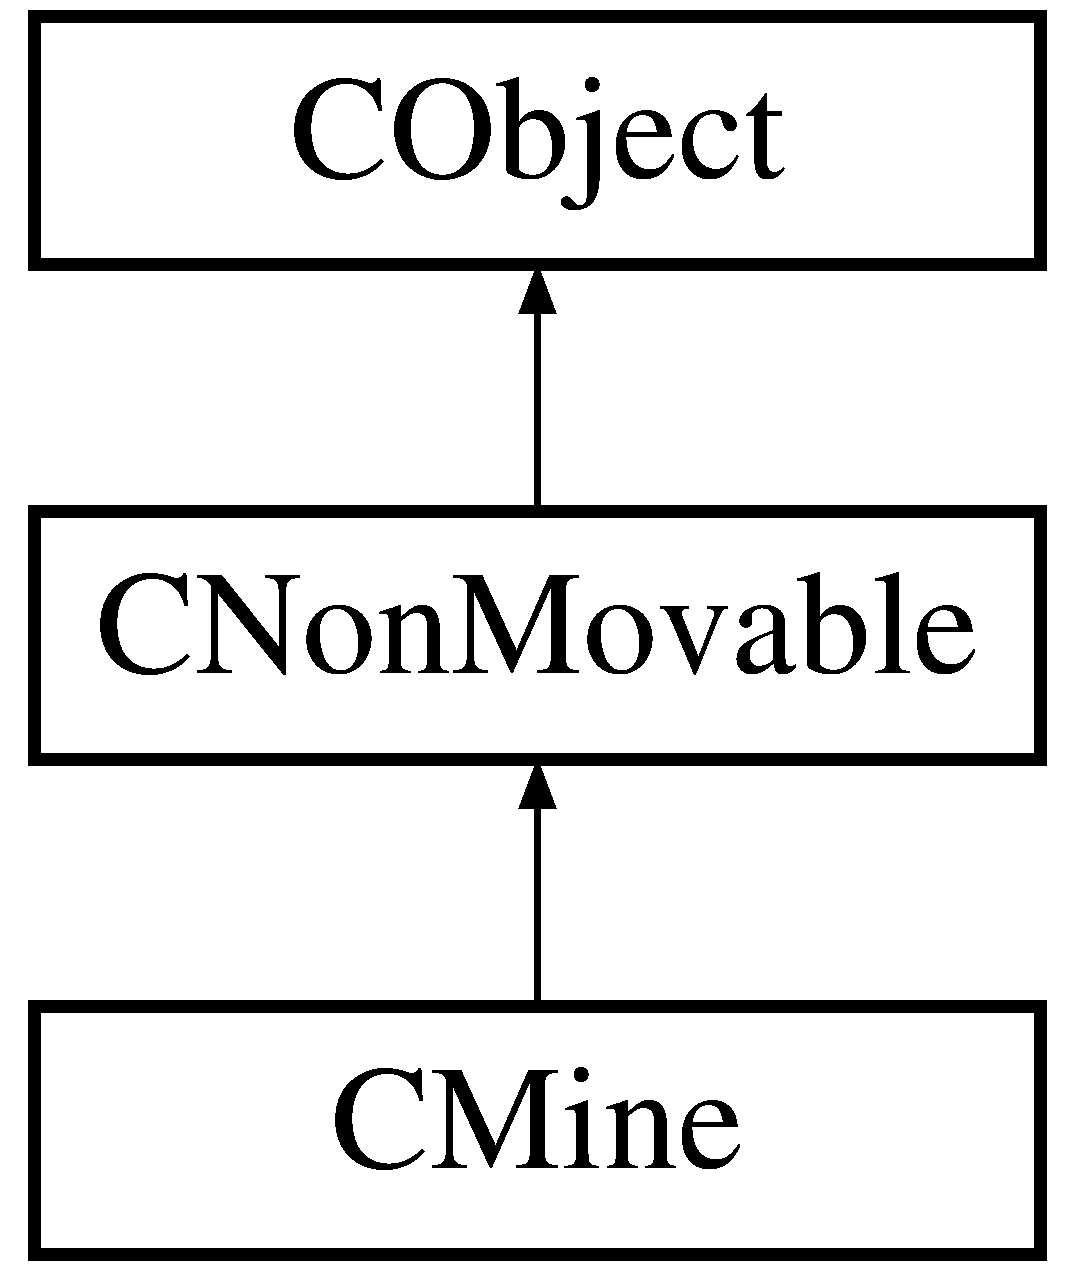
\includegraphics[height=3.000000cm]{class_c_mine}
\end{center}
\end{figure}
\subsection*{Public Member Functions}
\begin{DoxyCompactItemize}
\item 
\mbox{\hyperlink{class_c_mine_ab9f50e2a84a1e768155a2554b629d03d}{C\+Mine}} (\mbox{\hyperlink{class_c_map}{C\+Map}} $\ast$m)
\item 
virtual \mbox{\hyperlink{class_c_mine_ae19438d30c9e697e7911aab5901e1192}{$\sim$\+C\+Mine}} ()
\item 
void \mbox{\hyperlink{class_c_mine_aef4825eff1e61d284d3da7a2d630acb5}{update}} ()
\begin{DoxyCompactList}\small\item\em Sprawdza, czy z miną kolidują jakieś roboty. \end{DoxyCompactList}\item 
void \mbox{\hyperlink{class_c_mine_ae7ecce2601b654160e8bd4edf84723ee}{destroy}} (std\+::vector$<$ \mbox{\hyperlink{class_c_robot}{C\+Robot}} $\ast$$>$ robots)
\begin{DoxyCompactList}\small\item\em Niszczy robota kolidującego z miną \end{DoxyCompactList}\end{DoxyCompactItemize}
\subsection*{Additional Inherited Members}


\subsection{Detailed Description}
Mina niszcząca roboty, które na nią wpadną 

\subsection{Constructor \& Destructor Documentation}
\mbox{\Hypertarget{class_c_mine_ab9f50e2a84a1e768155a2554b629d03d}\label{class_c_mine_ab9f50e2a84a1e768155a2554b629d03d}} 
\index{C\+Mine@{C\+Mine}!C\+Mine@{C\+Mine}}
\index{C\+Mine@{C\+Mine}!C\+Mine@{C\+Mine}}
\subsubsection{\texorpdfstring{C\+Mine()}{CMine()}}
{\footnotesize\ttfamily C\+Mine\+::\+C\+Mine (\begin{DoxyParamCaption}\item[{\mbox{\hyperlink{class_c_map}{C\+Map}} $\ast$}]{m }\end{DoxyParamCaption})}

\mbox{\Hypertarget{class_c_mine_ae19438d30c9e697e7911aab5901e1192}\label{class_c_mine_ae19438d30c9e697e7911aab5901e1192}} 
\index{C\+Mine@{C\+Mine}!````~C\+Mine@{$\sim$\+C\+Mine}}
\index{````~C\+Mine@{$\sim$\+C\+Mine}!C\+Mine@{C\+Mine}}
\subsubsection{\texorpdfstring{$\sim$\+C\+Mine()}{~CMine()}}
{\footnotesize\ttfamily C\+Mine\+::$\sim$\+C\+Mine (\begin{DoxyParamCaption}{ }\end{DoxyParamCaption})\hspace{0.3cm}{\ttfamily [virtual]}}



\subsection{Member Function Documentation}
\mbox{\Hypertarget{class_c_mine_ae7ecce2601b654160e8bd4edf84723ee}\label{class_c_mine_ae7ecce2601b654160e8bd4edf84723ee}} 
\index{C\+Mine@{C\+Mine}!destroy@{destroy}}
\index{destroy@{destroy}!C\+Mine@{C\+Mine}}
\subsubsection{\texorpdfstring{destroy()}{destroy()}}
{\footnotesize\ttfamily void C\+Mine\+::destroy (\begin{DoxyParamCaption}\item[{std\+::vector$<$ \mbox{\hyperlink{class_c_robot}{C\+Robot}} $\ast$$>$}]{robots }\end{DoxyParamCaption})}



Niszczy robota kolidującego z miną 


\begin{DoxyParams}{Parameters}
{\em robots} & Robot, którego należy usunąć \\
\hline
\end{DoxyParams}
\mbox{\Hypertarget{class_c_mine_aef4825eff1e61d284d3da7a2d630acb5}\label{class_c_mine_aef4825eff1e61d284d3da7a2d630acb5}} 
\index{C\+Mine@{C\+Mine}!update@{update}}
\index{update@{update}!C\+Mine@{C\+Mine}}
\subsubsection{\texorpdfstring{update()}{update()}}
{\footnotesize\ttfamily void C\+Mine\+::update (\begin{DoxyParamCaption}{ }\end{DoxyParamCaption})\hspace{0.3cm}{\ttfamily [virtual]}}



Sprawdza, czy z miną kolidują jakieś roboty. 



Implements \mbox{\hyperlink{class_c_non_movable_ace03bea0246940c6c5c0b26ffa1ef165}{C\+Non\+Movable}}.



The documentation for this class was generated from the following files\+:\begin{DoxyCompactItemize}
\item 
\mbox{\hyperlink{cmine_8h}{cmine.\+h}}\item 
\mbox{\hyperlink{cmine_8cpp}{cmine.\+cpp}}\end{DoxyCompactItemize}

\hypertarget{class_c_movable}{}\section{C\+Movable Class Reference}
\label{class_c_movable}\index{C\+Movable@{C\+Movable}}


Klasa reprezentująca obiekty z możliwością poruszania się po mapie.  




{\ttfamily \#include $<$cmovable.\+h$>$}

Inheritance diagram for C\+Movable\+:\begin{figure}[H]
\begin{center}
\leavevmode
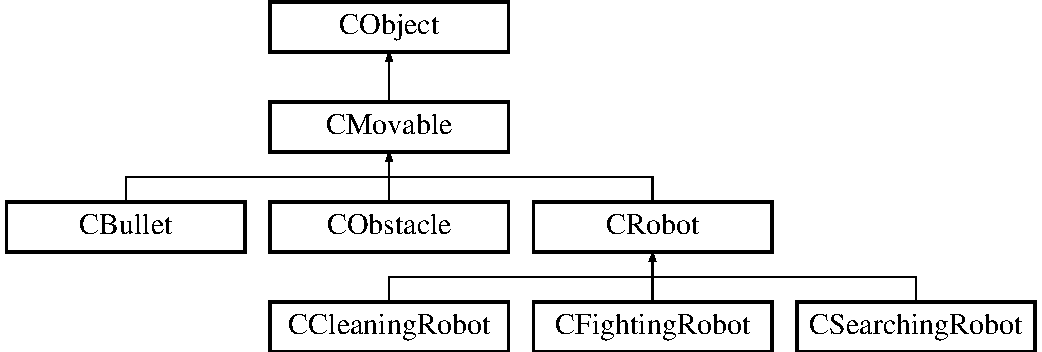
\includegraphics[height=4.000000cm]{class_c_movable}
\end{center}
\end{figure}
\subsection*{Public Member Functions}
\begin{DoxyCompactItemize}
\item 
\mbox{\hyperlink{class_c_movable_a5f049731afad44da86ff6e3684c258e9}{C\+Movable}} (qreal xv, qreal yv, qreal anglev, qreal rangev, \mbox{\hyperlink{class_c_map}{C\+Map}} $\ast$m)
\item 
virtual void \mbox{\hyperlink{class_c_movable_af45fc62960d86ef62949d078141e9d62}{update}} ()=0
\begin{DoxyCompactList}\small\item\em Funkcja wywoływana przy każdym kroku programu dla wszystkich obiektów, oddziaływuje na otoczenie oraz podejmuje decyzje na podstawie tego otoczenia, implementacja jest różna dla każdej z podklas na najniższym szczeblu hierarchii dziedziczenia. \end{DoxyCompactList}\item 
virtual void \mbox{\hyperlink{class_c_movable_a8e66e106f13362d24462ce0c9d0431af}{move}} ()=0
\begin{DoxyCompactList}\small\item\em Funkcja zmieniająca położenie obiektu przy każdym kroku; implementacja zależy od typu obieku. \end{DoxyCompactList}\end{DoxyCompactItemize}
\subsection*{Additional Inherited Members}


\subsection{Detailed Description}
Klasa reprezentująca obiekty z możliwością poruszania się po mapie. 

\subsection{Constructor \& Destructor Documentation}
\mbox{\Hypertarget{class_c_movable_a5f049731afad44da86ff6e3684c258e9}\label{class_c_movable_a5f049731afad44da86ff6e3684c258e9}} 
\index{C\+Movable@{C\+Movable}!C\+Movable@{C\+Movable}}
\index{C\+Movable@{C\+Movable}!C\+Movable@{C\+Movable}}
\subsubsection{\texorpdfstring{C\+Movable()}{CMovable()}}
{\footnotesize\ttfamily C\+Movable\+::\+C\+Movable (\begin{DoxyParamCaption}\item[{qreal}]{xv,  }\item[{qreal}]{yv,  }\item[{qreal}]{anglev,  }\item[{qreal}]{rangev,  }\item[{\mbox{\hyperlink{class_c_map}{C\+Map}} $\ast$}]{m }\end{DoxyParamCaption})}



\subsection{Member Function Documentation}
\mbox{\Hypertarget{class_c_movable_a8e66e106f13362d24462ce0c9d0431af}\label{class_c_movable_a8e66e106f13362d24462ce0c9d0431af}} 
\index{C\+Movable@{C\+Movable}!move@{move}}
\index{move@{move}!C\+Movable@{C\+Movable}}
\subsubsection{\texorpdfstring{move()}{move()}}
{\footnotesize\ttfamily virtual void C\+Movable\+::move (\begin{DoxyParamCaption}{ }\end{DoxyParamCaption})\hspace{0.3cm}{\ttfamily [pure virtual]}}



Funkcja zmieniająca położenie obiektu przy każdym kroku; implementacja zależy od typu obieku. 



Implemented in \mbox{\hyperlink{class_c_bullet_a693e95f219a9a642e3977bb48be0cf5d}{C\+Bullet}}, \mbox{\hyperlink{class_c_robot_a1de9be879213eadf7ded27caedb84598}{C\+Robot}}, \mbox{\hyperlink{class_c_obstacle_a4b2e4989c993dd7f79cd66fd485c3c88}{C\+Obstacle}}, \mbox{\hyperlink{class_c_cleaning_robot_a1ad227a5f3508a8e78fcecae7d3de53b}{C\+Cleaning\+Robot}}, \mbox{\hyperlink{class_c_searching_robot_a2c2150e7fd1cefbb5851e039cd76572f}{C\+Searching\+Robot}}, and \mbox{\hyperlink{class_c_fighting_robot_af644acbba178e256566e9dbd230aa4db}{C\+Fighting\+Robot}}.

\mbox{\Hypertarget{class_c_movable_af45fc62960d86ef62949d078141e9d62}\label{class_c_movable_af45fc62960d86ef62949d078141e9d62}} 
\index{C\+Movable@{C\+Movable}!update@{update}}
\index{update@{update}!C\+Movable@{C\+Movable}}
\subsubsection{\texorpdfstring{update()}{update()}}
{\footnotesize\ttfamily virtual void C\+Movable\+::update (\begin{DoxyParamCaption}{ }\end{DoxyParamCaption})\hspace{0.3cm}{\ttfamily [pure virtual]}}



Funkcja wywoływana przy każdym kroku programu dla wszystkich obiektów, oddziaływuje na otoczenie oraz podejmuje decyzje na podstawie tego otoczenia, implementacja jest różna dla każdej z podklas na najniższym szczeblu hierarchii dziedziczenia. 



Implements \mbox{\hyperlink{class_c_object_acb42ca516e836d0267ddb9a0556916a9}{C\+Object}}.



Implemented in \mbox{\hyperlink{class_c_bullet_a9685917f7fc76d417e03744223b1b2c6}{C\+Bullet}}, \mbox{\hyperlink{class_c_robot_a8ad8d55a840ced20f85a2a045e9e24ef}{C\+Robot}}, \mbox{\hyperlink{class_c_cleaning_robot_afd8b3a58abfc91ebdce32af3686c5e9f}{C\+Cleaning\+Robot}}, \mbox{\hyperlink{class_c_searching_robot_a6e9cdc9eccd32a470d8953f1a3cccd46}{C\+Searching\+Robot}}, \mbox{\hyperlink{class_c_fighting_robot_a3ae0ea383f809766e53c81348a07daaa}{C\+Fighting\+Robot}}, and \mbox{\hyperlink{class_c_obstacle_a9aeb124d28bdef3430954f5e2b5ae0f0}{C\+Obstacle}}.



The documentation for this class was generated from the following files\+:\begin{DoxyCompactItemize}
\item 
\mbox{\hyperlink{cmovable_8h}{cmovable.\+h}}\item 
\mbox{\hyperlink{cmovable_8cpp}{cmovable.\+cpp}}\end{DoxyCompactItemize}

\hypertarget{class_c_non_movable}{}\section{C\+Non\+Movable Class Reference}
\label{class_c_non_movable}\index{C\+Non\+Movable@{C\+Non\+Movable}}


Klasa reprezentująca nieruchome obiekty na mapie.  




{\ttfamily \#include $<$cnonmovable.\+h$>$}

Inheritance diagram for C\+Non\+Movable\+:\begin{figure}[H]
\begin{center}
\leavevmode
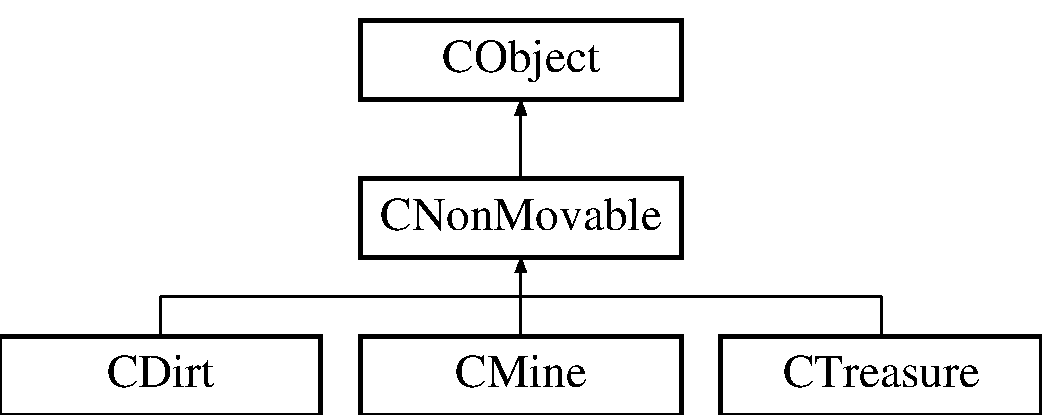
\includegraphics[height=3.000000cm]{class_c_non_movable}
\end{center}
\end{figure}
\subsection*{Public Member Functions}
\begin{DoxyCompactItemize}
\item 
\mbox{\hyperlink{class_c_non_movable_abe455ba26ac2d5b3eb5e99e7a282b9b7}{C\+Non\+Movable}} (qreal xv, qreal yv, qreal anglev, qreal rangev, qreal valuev, \mbox{\hyperlink{class_c_map}{C\+Map}} $\ast$m)
\item 
qreal \mbox{\hyperlink{class_c_non_movable_a34204726d749b5eb66ed763119a46163}{getvalue}} ()
\begin{DoxyCompactList}\small\item\em Funkcja zwracająca wartość value. \end{DoxyCompactList}\item 
virtual void \mbox{\hyperlink{class_c_non_movable_ace03bea0246940c6c5c0b26ffa1ef165}{update}} ()=0
\begin{DoxyCompactList}\small\item\em Funkcja wywoływana przy każdym kroku programu dla wszystkich obiektów, oddziaływuje na otoczenie oraz podejmuje decyzje na podstawie tego otoczenia, implementacja jest różna dla każdej z podklas na najniższym szczeblu hierarchii dziedziczenia. \end{DoxyCompactList}\end{DoxyCompactItemize}
\subsection*{Protected Attributes}
\begin{DoxyCompactItemize}
\item 
qreal \mbox{\hyperlink{class_c_non_movable_aaa6f737556a51a132b8cc89255b8c096}{value}}
\begin{DoxyCompactList}\small\item\em Zmienna reprezentująca wielkość danego obiektu lub jego wartość \end{DoxyCompactList}\end{DoxyCompactItemize}


\subsection{Detailed Description}
Klasa reprezentująca nieruchome obiekty na mapie. 

\subsection{Constructor \& Destructor Documentation}
\mbox{\Hypertarget{class_c_non_movable_abe455ba26ac2d5b3eb5e99e7a282b9b7}\label{class_c_non_movable_abe455ba26ac2d5b3eb5e99e7a282b9b7}} 
\index{C\+Non\+Movable@{C\+Non\+Movable}!C\+Non\+Movable@{C\+Non\+Movable}}
\index{C\+Non\+Movable@{C\+Non\+Movable}!C\+Non\+Movable@{C\+Non\+Movable}}
\subsubsection{\texorpdfstring{C\+Non\+Movable()}{CNonMovable()}}
{\footnotesize\ttfamily C\+Non\+Movable\+::\+C\+Non\+Movable (\begin{DoxyParamCaption}\item[{qreal}]{xv,  }\item[{qreal}]{yv,  }\item[{qreal}]{anglev,  }\item[{qreal}]{rangev,  }\item[{qreal}]{valuev,  }\item[{\mbox{\hyperlink{class_c_map}{C\+Map}} $\ast$}]{m }\end{DoxyParamCaption})}



\subsection{Member Function Documentation}
\mbox{\Hypertarget{class_c_non_movable_a34204726d749b5eb66ed763119a46163}\label{class_c_non_movable_a34204726d749b5eb66ed763119a46163}} 
\index{C\+Non\+Movable@{C\+Non\+Movable}!getvalue@{getvalue}}
\index{getvalue@{getvalue}!C\+Non\+Movable@{C\+Non\+Movable}}
\subsubsection{\texorpdfstring{getvalue()}{getvalue()}}
{\footnotesize\ttfamily qreal C\+Non\+Movable\+::getvalue (\begin{DoxyParamCaption}{ }\end{DoxyParamCaption})}



Funkcja zwracająca wartość value. 

\begin{DoxyReturn}{Returns}
value 
\end{DoxyReturn}
\mbox{\Hypertarget{class_c_non_movable_ace03bea0246940c6c5c0b26ffa1ef165}\label{class_c_non_movable_ace03bea0246940c6c5c0b26ffa1ef165}} 
\index{C\+Non\+Movable@{C\+Non\+Movable}!update@{update}}
\index{update@{update}!C\+Non\+Movable@{C\+Non\+Movable}}
\subsubsection{\texorpdfstring{update()}{update()}}
{\footnotesize\ttfamily virtual void C\+Non\+Movable\+::update (\begin{DoxyParamCaption}{ }\end{DoxyParamCaption})\hspace{0.3cm}{\ttfamily [pure virtual]}}



Funkcja wywoływana przy każdym kroku programu dla wszystkich obiektów, oddziaływuje na otoczenie oraz podejmuje decyzje na podstawie tego otoczenia, implementacja jest różna dla każdej z podklas na najniższym szczeblu hierarchii dziedziczenia. 



Implements \mbox{\hyperlink{class_c_object_acb42ca516e836d0267ddb9a0556916a9}{C\+Object}}.



Implemented in \mbox{\hyperlink{class_c_mine_aef4825eff1e61d284d3da7a2d630acb5}{C\+Mine}}, \mbox{\hyperlink{class_c_dirt_a0f077e7fde1b397f08659f65d28cf573}{C\+Dirt}}, and \mbox{\hyperlink{class_c_treasure_a5030f2a7279aa608c40741f9e7040a90}{C\+Treasure}}.



\subsection{Member Data Documentation}
\mbox{\Hypertarget{class_c_non_movable_aaa6f737556a51a132b8cc89255b8c096}\label{class_c_non_movable_aaa6f737556a51a132b8cc89255b8c096}} 
\index{C\+Non\+Movable@{C\+Non\+Movable}!value@{value}}
\index{value@{value}!C\+Non\+Movable@{C\+Non\+Movable}}
\subsubsection{\texorpdfstring{value}{value}}
{\footnotesize\ttfamily qreal C\+Non\+Movable\+::value\hspace{0.3cm}{\ttfamily [protected]}}



Zmienna reprezentująca wielkość danego obiektu lub jego wartość 



The documentation for this class was generated from the following files\+:\begin{DoxyCompactItemize}
\item 
\mbox{\hyperlink{cnonmovable_8h}{cnonmovable.\+h}}\item 
\mbox{\hyperlink{cnonmovable_8cpp}{cnonmovable.\+cpp}}\end{DoxyCompactItemize}

\hypertarget{class_c_object}{}\section{C\+Object Class Reference}
\label{class_c_object}\index{C\+Object@{C\+Object}}


Klasa reprezentująca każdy obiekt na mapie.  




{\ttfamily \#include $<$cobject.\+h$>$}

Inheritance diagram for C\+Object\+:\begin{figure}[H]
\begin{center}
\leavevmode
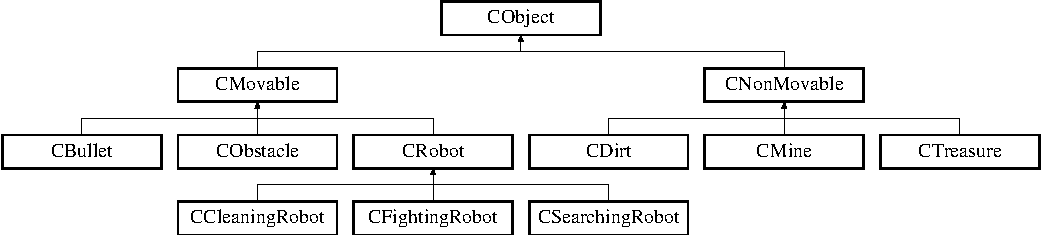
\includegraphics[height=3.137255cm]{class_c_object}
\end{center}
\end{figure}
\subsection*{Public Member Functions}
\begin{DoxyCompactItemize}
\item 
\mbox{\hyperlink{class_c_object_ab8bac765156b93002423cd43e853611f}{C\+Object}} (qreal xv, qreal yv, qreal anglev, qreal rangev, \mbox{\hyperlink{class_c_map}{C\+Map}} $\ast$m)
\begin{DoxyCompactList}\small\item\em Konstruktor pozwala tylko na stworzenie obiektu o konkretnych parametrach; kształt obiektu określany jest przez konstruktory klas dziedziczących w zależności od rodzaju obiektu. \end{DoxyCompactList}\item 
virtual void \mbox{\hyperlink{class_c_object_acb42ca516e836d0267ddb9a0556916a9}{update}} ()=0
\begin{DoxyCompactList}\small\item\em Funkcja wywoływana przy każdym kroku programu dla wszystkich obiektów, oddziaływuje na otoczenie oraz podejmuje decyzje na podstawie tego otoczenia, implementacja jest różna dla każdej z podklas na najniższym szczeblu hierarchii dziedziczenia. \end{DoxyCompactList}\item 
qreal \mbox{\hyperlink{class_c_object_a9199c97746518fd8eb029033d7539fbb}{getX}} ()
\begin{DoxyCompactList}\small\item\em Zwraca wartość współrzędnej x obiektu. \end{DoxyCompactList}\item 
qreal \mbox{\hyperlink{class_c_object_ac9ce72541d4420b65ec5abf7478f6e62}{getY}} ()
\begin{DoxyCompactList}\small\item\em Zwraca wartość współrzędnej y obiektu. \end{DoxyCompactList}\item 
qreal \mbox{\hyperlink{class_c_object_af1c8e71b2974e222f4b164f70dd7ffc4}{get\+Angle}} ()
\begin{DoxyCompactList}\small\item\em Zwraca kąt, pod jakim znajduje się obiekt(w radianach) \end{DoxyCompactList}\item 
qreal \mbox{\hyperlink{class_c_object_a8d0881ca2211266500a3d4af11cf8824}{get\+Range}} ()
\begin{DoxyCompactList}\small\item\em Zwraca zasięg obiektu. \end{DoxyCompactList}\item 
\mbox{\hyperlink{class_c_map}{C\+Map}} $\ast$ \mbox{\hyperlink{class_c_object_a57ea53dbd6d12a6da554f24d7b6c0d5d}{get\+Map}} ()
\begin{DoxyCompactList}\small\item\em Zwraca wskaźnik do mapy, na której znajduje się obiekt. \end{DoxyCompactList}\item 
qreal \mbox{\hyperlink{class_c_object_ad8e89183e35939476e2c6e0afb832f89}{get\+Width}} ()
\begin{DoxyCompactList}\small\item\em Zwraca szerokość obiektu. \end{DoxyCompactList}\item 
qreal \mbox{\hyperlink{class_c_object_ab1f242475368097db1eea253b9cc77e1}{get\+Height}} ()
\begin{DoxyCompactList}\small\item\em Zwraca wysokość obiektu. \end{DoxyCompactList}\item 
\mbox{\hyperlink{cobject_8h_a45cde9abb508c62d67c3bb2b9bf566a5}{shape}} \mbox{\hyperlink{class_c_object_aca839368d91bd68f3d46288316a86807}{get\+Shape}} ()
\begin{DoxyCompactList}\small\item\em Zwraca kształt obiektu. \end{DoxyCompactList}\item 
qreal \mbox{\hyperlink{class_c_object_a451ca4149ae1de4dfe39370c3abbe919}{distance}} (\mbox{\hyperlink{class_c_object}{C\+Object}} $\ast$o)
\begin{DoxyCompactList}\small\item\em Zwraca odległość między obiektem, dla którego wywoływana jest metoda oraz obiektem, do którego przyjmuje wskaźnik. \end{DoxyCompactList}\item 
qreal \mbox{\hyperlink{class_c_object_aabaf82a62b691b0666a0bbe9431d3b22}{collision\+Distance}} (\mbox{\hyperlink{class_c_object}{C\+Object}} $\ast$o)
\begin{DoxyCompactList}\small\item\em Na podstawie kształtu obiektów oblicza maksymalną odległość, przy której nie kolidują one ze sobą \end{DoxyCompactList}\item 
bool \mbox{\hyperlink{class_c_object_ad744a67920a169209f631f9e34f1d891}{collides\+With}} (\mbox{\hyperlink{class_c_object}{C\+Object}} $\ast$o)
\begin{DoxyCompactList}\small\item\em Zwraca informację o tym, czy dany obiekt koliduje z obiektem, dla którego wywoływana jest metoda. \end{DoxyCompactList}\item 
bool \mbox{\hyperlink{class_c_object_a24bf5bc6cf7e76478ac7ccc7c79cdd72}{will\+Collide}} (\mbox{\hyperlink{class_c_object}{C\+Object}} $\ast$o, qreal this\+Speed, qreal o\+Speed)
\begin{DoxyCompactList}\small\item\em Zwraca informację o tym, czy dwa obiekty o różnych prędkościach po wykonaniu ruchu będą ze sobą kolidować \end{DoxyCompactList}\end{DoxyCompactItemize}
\subsection*{Protected Attributes}
\begin{DoxyCompactItemize}
\item 
qreal \mbox{\hyperlink{class_c_object_acb23178c7b65e6cf37f9ab95128cd8d2}{x}}
\begin{DoxyCompactList}\small\item\em Współrzędna x. \end{DoxyCompactList}\item 
qreal \mbox{\hyperlink{class_c_object_a22fd03bdf2bc5c7058e4c2a9c9237c64}{y}}
\begin{DoxyCompactList}\small\item\em Współrzędna y. \end{DoxyCompactList}\item 
qreal \mbox{\hyperlink{class_c_object_a9ac381be23878447d48800b16d773efa}{angle}}
\begin{DoxyCompactList}\small\item\em Orientacja obiektu. \end{DoxyCompactList}\item 
qreal \mbox{\hyperlink{class_c_object_a0d3f8546df4d7620602646e7661d905e}{range}}
\begin{DoxyCompactList}\small\item\em Promień, w jakim obiekt może zauważać inne obiekty. \end{DoxyCompactList}\item 
\mbox{\hyperlink{class_c_map}{C\+Map}} $\ast$ \mbox{\hyperlink{class_c_object_a958cfe5f141fdab246af5da849f98d07}{map}}
\begin{DoxyCompactList}\small\item\em Wskaźnik na mapę, na której znajduje się obiekt. \end{DoxyCompactList}\item 
\mbox{\hyperlink{cobject_8h_a45cde9abb508c62d67c3bb2b9bf566a5}{shape}} \mbox{\hyperlink{class_c_object_a97a0d16c78ba0afc53f6df41055e6d94}{object\+Shape}}
\begin{DoxyCompactList}\small\item\em Kształt obiektu używany przy obliczaniu kolizji. \end{DoxyCompactList}\item 
qreal \mbox{\hyperlink{class_c_object_a6fceaa9b662c540109880306373fef4a}{width}}
\begin{DoxyCompactList}\small\item\em Szerokość obiektu. \end{DoxyCompactList}\item 
qreal \mbox{\hyperlink{class_c_object_a80f942a5fb6676096b7ab105842a6bd3}{height}}
\begin{DoxyCompactList}\small\item\em Wysokość obiektu. \end{DoxyCompactList}\end{DoxyCompactItemize}


\subsection{Detailed Description}
Klasa reprezentująca każdy obiekt na mapie. 

\subsection{Constructor \& Destructor Documentation}
\mbox{\Hypertarget{class_c_object_ab8bac765156b93002423cd43e853611f}\label{class_c_object_ab8bac765156b93002423cd43e853611f}} 
\index{C\+Object@{C\+Object}!C\+Object@{C\+Object}}
\index{C\+Object@{C\+Object}!C\+Object@{C\+Object}}
\subsubsection{\texorpdfstring{C\+Object()}{CObject()}}
{\footnotesize\ttfamily C\+Object\+::\+C\+Object (\begin{DoxyParamCaption}\item[{qreal}]{xv,  }\item[{qreal}]{yv,  }\item[{qreal}]{anglev,  }\item[{qreal}]{rangev,  }\item[{\mbox{\hyperlink{class_c_map}{C\+Map}} $\ast$}]{m }\end{DoxyParamCaption})}



Konstruktor pozwala tylko na stworzenie obiektu o konkretnych parametrach; kształt obiektu określany jest przez konstruktory klas dziedziczących w zależności od rodzaju obiektu. 


\begin{DoxyParams}{Parameters}
{\em xv} & Współrzędna x \\
\hline
{\em yv} & Współrzędna y \\
\hline
{\em anglev} & Orientacja obiektu \\
\hline
{\em rangev} & Zasięg obiektu \\
\hline
{\em m} & Wskaźnik na mapę, na której znajduje się obiekt \\
\hline
\end{DoxyParams}


\subsection{Member Function Documentation}
\mbox{\Hypertarget{class_c_object_ad744a67920a169209f631f9e34f1d891}\label{class_c_object_ad744a67920a169209f631f9e34f1d891}} 
\index{C\+Object@{C\+Object}!collides\+With@{collides\+With}}
\index{collides\+With@{collides\+With}!C\+Object@{C\+Object}}
\subsubsection{\texorpdfstring{collides\+With()}{collidesWith()}}
{\footnotesize\ttfamily bool C\+Object\+::collides\+With (\begin{DoxyParamCaption}\item[{\mbox{\hyperlink{class_c_object}{C\+Object}} $\ast$}]{o }\end{DoxyParamCaption})}



Zwraca informację o tym, czy dany obiekt koliduje z obiektem, dla którego wywoływana jest metoda. 


\begin{DoxyParams}{Parameters}
{\em o} & Obiekt, dla którego sprawdzana jest kolizja \\
\hline
\end{DoxyParams}
\begin{DoxyReturn}{Returns}
1 oznacza kolizję, 0 brak kolizji 
\end{DoxyReturn}
\mbox{\Hypertarget{class_c_object_aabaf82a62b691b0666a0bbe9431d3b22}\label{class_c_object_aabaf82a62b691b0666a0bbe9431d3b22}} 
\index{C\+Object@{C\+Object}!collision\+Distance@{collision\+Distance}}
\index{collision\+Distance@{collision\+Distance}!C\+Object@{C\+Object}}
\subsubsection{\texorpdfstring{collision\+Distance()}{collisionDistance()}}
{\footnotesize\ttfamily qreal C\+Object\+::collision\+Distance (\begin{DoxyParamCaption}\item[{\mbox{\hyperlink{class_c_object}{C\+Object}} $\ast$}]{o }\end{DoxyParamCaption})}



Na podstawie kształtu obiektów oblicza maksymalną odległość, przy której nie kolidują one ze sobą 


\begin{DoxyParams}{Parameters}
{\em o} & Obiekt, dla którego liczona jest odległość \\
\hline
\end{DoxyParams}
\begin{DoxyReturn}{Returns}
Dystans w metryce euklidesowej 
\end{DoxyReturn}
\mbox{\Hypertarget{class_c_object_a451ca4149ae1de4dfe39370c3abbe919}\label{class_c_object_a451ca4149ae1de4dfe39370c3abbe919}} 
\index{C\+Object@{C\+Object}!distance@{distance}}
\index{distance@{distance}!C\+Object@{C\+Object}}
\subsubsection{\texorpdfstring{distance()}{distance()}}
{\footnotesize\ttfamily qreal C\+Object\+::distance (\begin{DoxyParamCaption}\item[{\mbox{\hyperlink{class_c_object}{C\+Object}} $\ast$}]{o }\end{DoxyParamCaption})}



Zwraca odległość między obiektem, dla którego wywoływana jest metoda oraz obiektem, do którego przyjmuje wskaźnik. 


\begin{DoxyParams}{Parameters}
{\em o} & Obiekt, dla którego liczona jest odległość \\
\hline
\end{DoxyParams}
\begin{DoxyReturn}{Returns}
Dystans między obiektami w metryce euklidesowej 
\end{DoxyReturn}
\mbox{\Hypertarget{class_c_object_af1c8e71b2974e222f4b164f70dd7ffc4}\label{class_c_object_af1c8e71b2974e222f4b164f70dd7ffc4}} 
\index{C\+Object@{C\+Object}!get\+Angle@{get\+Angle}}
\index{get\+Angle@{get\+Angle}!C\+Object@{C\+Object}}
\subsubsection{\texorpdfstring{get\+Angle()}{getAngle()}}
{\footnotesize\ttfamily qreal C\+Object\+::get\+Angle (\begin{DoxyParamCaption}{ }\end{DoxyParamCaption})}



Zwraca kąt, pod jakim znajduje się obiekt(w radianach) 

\begin{DoxyReturn}{Returns}
angle 
\end{DoxyReturn}
\mbox{\Hypertarget{class_c_object_ab1f242475368097db1eea253b9cc77e1}\label{class_c_object_ab1f242475368097db1eea253b9cc77e1}} 
\index{C\+Object@{C\+Object}!get\+Height@{get\+Height}}
\index{get\+Height@{get\+Height}!C\+Object@{C\+Object}}
\subsubsection{\texorpdfstring{get\+Height()}{getHeight()}}
{\footnotesize\ttfamily qreal C\+Object\+::get\+Height (\begin{DoxyParamCaption}{ }\end{DoxyParamCaption})}



Zwraca wysokość obiektu. 

\begin{DoxyReturn}{Returns}
height 
\end{DoxyReturn}
\mbox{\Hypertarget{class_c_object_a57ea53dbd6d12a6da554f24d7b6c0d5d}\label{class_c_object_a57ea53dbd6d12a6da554f24d7b6c0d5d}} 
\index{C\+Object@{C\+Object}!get\+Map@{get\+Map}}
\index{get\+Map@{get\+Map}!C\+Object@{C\+Object}}
\subsubsection{\texorpdfstring{get\+Map()}{getMap()}}
{\footnotesize\ttfamily \mbox{\hyperlink{class_c_map}{C\+Map}} $\ast$ C\+Object\+::get\+Map (\begin{DoxyParamCaption}{ }\end{DoxyParamCaption})}



Zwraca wskaźnik do mapy, na której znajduje się obiekt. 

\begin{DoxyReturn}{Returns}
map 
\end{DoxyReturn}
\mbox{\Hypertarget{class_c_object_a8d0881ca2211266500a3d4af11cf8824}\label{class_c_object_a8d0881ca2211266500a3d4af11cf8824}} 
\index{C\+Object@{C\+Object}!get\+Range@{get\+Range}}
\index{get\+Range@{get\+Range}!C\+Object@{C\+Object}}
\subsubsection{\texorpdfstring{get\+Range()}{getRange()}}
{\footnotesize\ttfamily qreal C\+Object\+::get\+Range (\begin{DoxyParamCaption}{ }\end{DoxyParamCaption})}



Zwraca zasięg obiektu. 

\begin{DoxyReturn}{Returns}
range 
\end{DoxyReturn}
\mbox{\Hypertarget{class_c_object_aca839368d91bd68f3d46288316a86807}\label{class_c_object_aca839368d91bd68f3d46288316a86807}} 
\index{C\+Object@{C\+Object}!get\+Shape@{get\+Shape}}
\index{get\+Shape@{get\+Shape}!C\+Object@{C\+Object}}
\subsubsection{\texorpdfstring{get\+Shape()}{getShape()}}
{\footnotesize\ttfamily int C\+Object\+::get\+Shape (\begin{DoxyParamCaption}{ }\end{DoxyParamCaption})}



Zwraca kształt obiektu. 

\begin{DoxyReturn}{Returns}
shape 
\end{DoxyReturn}
\mbox{\Hypertarget{class_c_object_ad8e89183e35939476e2c6e0afb832f89}\label{class_c_object_ad8e89183e35939476e2c6e0afb832f89}} 
\index{C\+Object@{C\+Object}!get\+Width@{get\+Width}}
\index{get\+Width@{get\+Width}!C\+Object@{C\+Object}}
\subsubsection{\texorpdfstring{get\+Width()}{getWidth()}}
{\footnotesize\ttfamily qreal C\+Object\+::get\+Width (\begin{DoxyParamCaption}{ }\end{DoxyParamCaption})}



Zwraca szerokość obiektu. 

\begin{DoxyReturn}{Returns}
width 
\end{DoxyReturn}
\mbox{\Hypertarget{class_c_object_a9199c97746518fd8eb029033d7539fbb}\label{class_c_object_a9199c97746518fd8eb029033d7539fbb}} 
\index{C\+Object@{C\+Object}!getX@{getX}}
\index{getX@{getX}!C\+Object@{C\+Object}}
\subsubsection{\texorpdfstring{get\+X()}{getX()}}
{\footnotesize\ttfamily qreal C\+Object\+::getX (\begin{DoxyParamCaption}{ }\end{DoxyParamCaption})}



Zwraca wartość współrzędnej x obiektu. 

\begin{DoxyReturn}{Returns}
x 
\end{DoxyReturn}
\mbox{\Hypertarget{class_c_object_ac9ce72541d4420b65ec5abf7478f6e62}\label{class_c_object_ac9ce72541d4420b65ec5abf7478f6e62}} 
\index{C\+Object@{C\+Object}!getY@{getY}}
\index{getY@{getY}!C\+Object@{C\+Object}}
\subsubsection{\texorpdfstring{get\+Y()}{getY()}}
{\footnotesize\ttfamily qreal C\+Object\+::getY (\begin{DoxyParamCaption}{ }\end{DoxyParamCaption})}



Zwraca wartość współrzędnej y obiektu. 

\begin{DoxyReturn}{Returns}
y 
\end{DoxyReturn}
\mbox{\Hypertarget{class_c_object_acb42ca516e836d0267ddb9a0556916a9}\label{class_c_object_acb42ca516e836d0267ddb9a0556916a9}} 
\index{C\+Object@{C\+Object}!update@{update}}
\index{update@{update}!C\+Object@{C\+Object}}
\subsubsection{\texorpdfstring{update()}{update()}}
{\footnotesize\ttfamily virtual void C\+Object\+::update (\begin{DoxyParamCaption}{ }\end{DoxyParamCaption})\hspace{0.3cm}{\ttfamily [pure virtual]}}



Funkcja wywoływana przy każdym kroku programu dla wszystkich obiektów, oddziaływuje na otoczenie oraz podejmuje decyzje na podstawie tego otoczenia, implementacja jest różna dla każdej z podklas na najniższym szczeblu hierarchii dziedziczenia. 



Implemented in \mbox{\hyperlink{class_c_bullet_a9685917f7fc76d417e03744223b1b2c6}{C\+Bullet}}, \mbox{\hyperlink{class_c_robot_a8ad8d55a840ced20f85a2a045e9e24ef}{C\+Robot}}, \mbox{\hyperlink{class_c_cleaning_robot_afd8b3a58abfc91ebdce32af3686c5e9f}{C\+Cleaning\+Robot}}, \mbox{\hyperlink{class_c_searching_robot_a6e9cdc9eccd32a470d8953f1a3cccd46}{C\+Searching\+Robot}}, \mbox{\hyperlink{class_c_fighting_robot_a3ae0ea383f809766e53c81348a07daaa}{C\+Fighting\+Robot}}, \mbox{\hyperlink{class_c_obstacle_a9aeb124d28bdef3430954f5e2b5ae0f0}{C\+Obstacle}}, \mbox{\hyperlink{class_c_non_movable_ace03bea0246940c6c5c0b26ffa1ef165}{C\+Non\+Movable}}, \mbox{\hyperlink{class_c_mine_aef4825eff1e61d284d3da7a2d630acb5}{C\+Mine}}, \mbox{\hyperlink{class_c_dirt_a0f077e7fde1b397f08659f65d28cf573}{C\+Dirt}}, \mbox{\hyperlink{class_c_treasure_a5030f2a7279aa608c40741f9e7040a90}{C\+Treasure}}, and \mbox{\hyperlink{class_c_movable_af45fc62960d86ef62949d078141e9d62}{C\+Movable}}.

\mbox{\Hypertarget{class_c_object_a24bf5bc6cf7e76478ac7ccc7c79cdd72}\label{class_c_object_a24bf5bc6cf7e76478ac7ccc7c79cdd72}} 
\index{C\+Object@{C\+Object}!will\+Collide@{will\+Collide}}
\index{will\+Collide@{will\+Collide}!C\+Object@{C\+Object}}
\subsubsection{\texorpdfstring{will\+Collide()}{willCollide()}}
{\footnotesize\ttfamily bool C\+Object\+::will\+Collide (\begin{DoxyParamCaption}\item[{\mbox{\hyperlink{class_c_object}{C\+Object}} $\ast$}]{o,  }\item[{qreal}]{this\+Speed,  }\item[{qreal}]{o\+Speed }\end{DoxyParamCaption})}



Zwraca informację o tym, czy dwa obiekty o różnych prędkościach po wykonaniu ruchu będą ze sobą kolidować 


\begin{DoxyParams}{Parameters}
{\em o} & Obiekt, dla którego sprawdzana jest ewentualna kolizja \\
\hline
{\em this\+Speed} & Prędkość, z jaką porusza się obiekt, dla którego wywoływana jest metoda \\
\hline
{\em o\+Speed} & Prędkość obiektu, dla którego sprawdazana jest kolizja \\
\hline
\end{DoxyParams}
\begin{DoxyReturn}{Returns}
1 oznacza kolizję w następnej turze, 0 oznacza jej brak 
\end{DoxyReturn}


\subsection{Member Data Documentation}
\mbox{\Hypertarget{class_c_object_a9ac381be23878447d48800b16d773efa}\label{class_c_object_a9ac381be23878447d48800b16d773efa}} 
\index{C\+Object@{C\+Object}!angle@{angle}}
\index{angle@{angle}!C\+Object@{C\+Object}}
\subsubsection{\texorpdfstring{angle}{angle}}
{\footnotesize\ttfamily qreal C\+Object\+::angle\hspace{0.3cm}{\ttfamily [protected]}}



Orientacja obiektu. 

\mbox{\Hypertarget{class_c_object_a80f942a5fb6676096b7ab105842a6bd3}\label{class_c_object_a80f942a5fb6676096b7ab105842a6bd3}} 
\index{C\+Object@{C\+Object}!height@{height}}
\index{height@{height}!C\+Object@{C\+Object}}
\subsubsection{\texorpdfstring{height}{height}}
{\footnotesize\ttfamily qreal C\+Object\+::height\hspace{0.3cm}{\ttfamily [protected]}}



Wysokość obiektu. 

\mbox{\Hypertarget{class_c_object_a958cfe5f141fdab246af5da849f98d07}\label{class_c_object_a958cfe5f141fdab246af5da849f98d07}} 
\index{C\+Object@{C\+Object}!map@{map}}
\index{map@{map}!C\+Object@{C\+Object}}
\subsubsection{\texorpdfstring{map}{map}}
{\footnotesize\ttfamily \mbox{\hyperlink{class_c_map}{C\+Map}}$\ast$ C\+Object\+::map\hspace{0.3cm}{\ttfamily [protected]}}



Wskaźnik na mapę, na której znajduje się obiekt. 

\mbox{\Hypertarget{class_c_object_a97a0d16c78ba0afc53f6df41055e6d94}\label{class_c_object_a97a0d16c78ba0afc53f6df41055e6d94}} 
\index{C\+Object@{C\+Object}!object\+Shape@{object\+Shape}}
\index{object\+Shape@{object\+Shape}!C\+Object@{C\+Object}}
\subsubsection{\texorpdfstring{object\+Shape}{objectShape}}
{\footnotesize\ttfamily \mbox{\hyperlink{cobject_8h_a45cde9abb508c62d67c3bb2b9bf566a5}{shape}} C\+Object\+::object\+Shape\hspace{0.3cm}{\ttfamily [protected]}}



Kształt obiektu używany przy obliczaniu kolizji. 

\mbox{\Hypertarget{class_c_object_a0d3f8546df4d7620602646e7661d905e}\label{class_c_object_a0d3f8546df4d7620602646e7661d905e}} 
\index{C\+Object@{C\+Object}!range@{range}}
\index{range@{range}!C\+Object@{C\+Object}}
\subsubsection{\texorpdfstring{range}{range}}
{\footnotesize\ttfamily qreal C\+Object\+::range\hspace{0.3cm}{\ttfamily [protected]}}



Promień, w jakim obiekt może zauważać inne obiekty. 

\mbox{\Hypertarget{class_c_object_a6fceaa9b662c540109880306373fef4a}\label{class_c_object_a6fceaa9b662c540109880306373fef4a}} 
\index{C\+Object@{C\+Object}!width@{width}}
\index{width@{width}!C\+Object@{C\+Object}}
\subsubsection{\texorpdfstring{width}{width}}
{\footnotesize\ttfamily qreal C\+Object\+::width\hspace{0.3cm}{\ttfamily [protected]}}



Szerokość obiektu. 

\mbox{\Hypertarget{class_c_object_acb23178c7b65e6cf37f9ab95128cd8d2}\label{class_c_object_acb23178c7b65e6cf37f9ab95128cd8d2}} 
\index{C\+Object@{C\+Object}!x@{x}}
\index{x@{x}!C\+Object@{C\+Object}}
\subsubsection{\texorpdfstring{x}{x}}
{\footnotesize\ttfamily qreal C\+Object\+::x\hspace{0.3cm}{\ttfamily [protected]}}



Współrzędna x. 

\mbox{\Hypertarget{class_c_object_a22fd03bdf2bc5c7058e4c2a9c9237c64}\label{class_c_object_a22fd03bdf2bc5c7058e4c2a9c9237c64}} 
\index{C\+Object@{C\+Object}!y@{y}}
\index{y@{y}!C\+Object@{C\+Object}}
\subsubsection{\texorpdfstring{y}{y}}
{\footnotesize\ttfamily qreal C\+Object\+::y\hspace{0.3cm}{\ttfamily [protected]}}



Współrzędna y. 



The documentation for this class was generated from the following files\+:\begin{DoxyCompactItemize}
\item 
\mbox{\hyperlink{cobject_8h}{cobject.\+h}}\item 
\mbox{\hyperlink{cobject_8cpp}{cobject.\+cpp}}\end{DoxyCompactItemize}

\hypertarget{class_c_obstacle}{}\section{C\+Obstacle Class Reference}
\label{class_c_obstacle}\index{C\+Obstacle@{C\+Obstacle}}


Przeszkody poruszające się po mapie po linii prostej.  




{\ttfamily \#include $<$cobstacle.\+h$>$}

Inheritance diagram for C\+Obstacle\+:\begin{figure}[H]
\begin{center}
\leavevmode
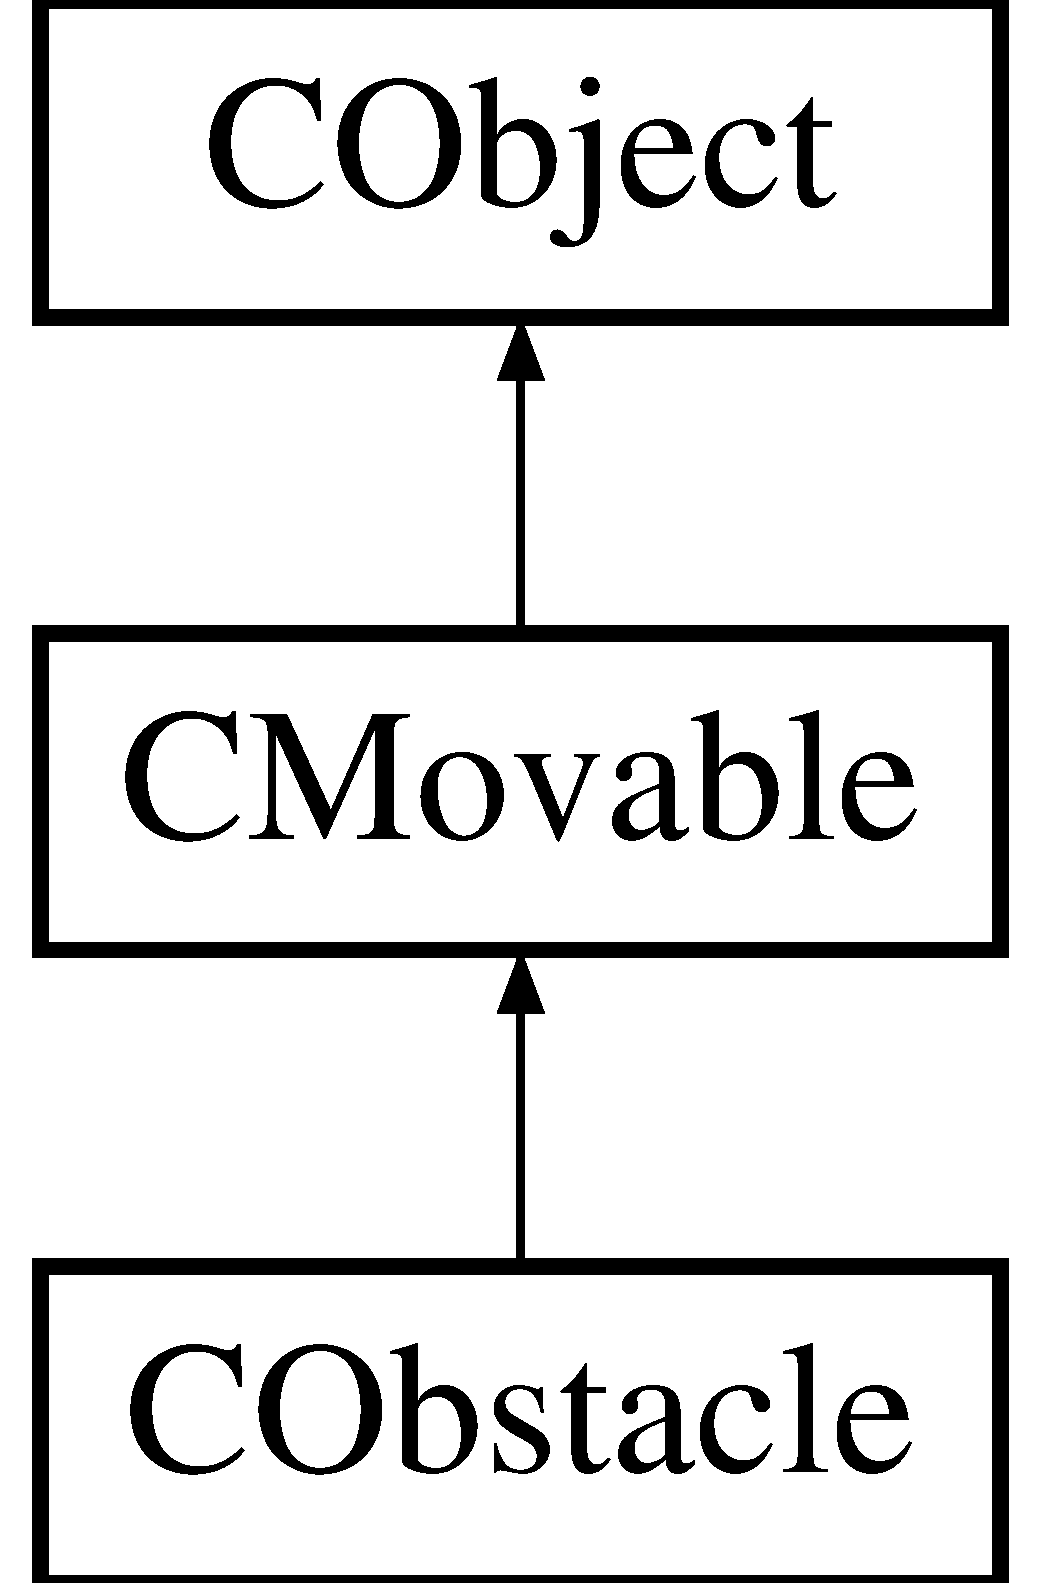
\includegraphics[height=3.000000cm]{class_c_obstacle}
\end{center}
\end{figure}
\subsection*{Public Member Functions}
\begin{DoxyCompactItemize}
\item 
\mbox{\hyperlink{class_c_obstacle_a3e105dc417eb5657e7cb1837259c235f}{C\+Obstacle}} (qreal xv, qreal yv, \mbox{\hyperlink{class_c_map}{C\+Map}} $\ast$m)
\item 
\mbox{\hyperlink{class_c_obstacle_ab1e0b16a38505ad38f085f7d87953c07}{C\+Obstacle}} (\mbox{\hyperlink{class_c_map}{C\+Map}} $\ast$m)
\item 
virtual \mbox{\hyperlink{class_c_obstacle_a10d5f9ec49321980b3cf46f868bc5f34}{$\sim$\+C\+Obstacle}} ()
\item 
void \mbox{\hyperlink{class_c_obstacle_a9aeb124d28bdef3430954f5e2b5ae0f0}{update}} ()
\begin{DoxyCompactList}\small\item\em Sprawdza, czy zajdzie kolizja z inną przeszkodą, jeśli tak, próbuje uniknąć kolizji(jedna z przeszkód zatrzymuje się); jeśli nastąpi kolizja z nieruchomym obiektem, obiekt ten jest niszczony; jeśli przeszkoda wyjdzie poza mapę, wywoływana jest funkcja \mbox{\hyperlink{class_c_obstacle_ae3aded0a2ac060a2124250a42ddacee4}{turn()}}; jeśli nie nastąpi kolizja z inną przeszkodą lub wyjście poza mapę, \mbox{\hyperlink{class_c_obstacle_a4b2e4989c993dd7f79cd66fd485c3c88}{move()}} \end{DoxyCompactList}\item 
void \mbox{\hyperlink{class_c_obstacle_a4b2e4989c993dd7f79cd66fd485c3c88}{move}} ()
\begin{DoxyCompactList}\small\item\em Zmienia współrzędne obiektu o odpowiednią prędkość w kierunku określonym przez jego orientację \end{DoxyCompactList}\item 
void \mbox{\hyperlink{class_c_obstacle_ae3aded0a2ac060a2124250a42ddacee4}{turn}} ()
\begin{DoxyCompactList}\small\item\em Odwraca obiekt o 180$\ast$. \end{DoxyCompactList}\end{DoxyCompactItemize}
\subsection*{Additional Inherited Members}


\subsection{Detailed Description}
Przeszkody poruszające się po mapie po linii prostej. 

\subsection{Constructor \& Destructor Documentation}
\mbox{\Hypertarget{class_c_obstacle_a3e105dc417eb5657e7cb1837259c235f}\label{class_c_obstacle_a3e105dc417eb5657e7cb1837259c235f}} 
\index{C\+Obstacle@{C\+Obstacle}!C\+Obstacle@{C\+Obstacle}}
\index{C\+Obstacle@{C\+Obstacle}!C\+Obstacle@{C\+Obstacle}}
\subsubsection{\texorpdfstring{C\+Obstacle()}{CObstacle()}\hspace{0.1cm}{\footnotesize\ttfamily [1/2]}}
{\footnotesize\ttfamily C\+Obstacle\+::\+C\+Obstacle (\begin{DoxyParamCaption}\item[{qreal}]{xv,  }\item[{qreal}]{yv,  }\item[{\mbox{\hyperlink{class_c_map}{C\+Map}} $\ast$}]{m }\end{DoxyParamCaption})}

\mbox{\Hypertarget{class_c_obstacle_ab1e0b16a38505ad38f085f7d87953c07}\label{class_c_obstacle_ab1e0b16a38505ad38f085f7d87953c07}} 
\index{C\+Obstacle@{C\+Obstacle}!C\+Obstacle@{C\+Obstacle}}
\index{C\+Obstacle@{C\+Obstacle}!C\+Obstacle@{C\+Obstacle}}
\subsubsection{\texorpdfstring{C\+Obstacle()}{CObstacle()}\hspace{0.1cm}{\footnotesize\ttfamily [2/2]}}
{\footnotesize\ttfamily C\+Obstacle\+::\+C\+Obstacle (\begin{DoxyParamCaption}\item[{\mbox{\hyperlink{class_c_map}{C\+Map}} $\ast$}]{m }\end{DoxyParamCaption})}

\mbox{\Hypertarget{class_c_obstacle_a10d5f9ec49321980b3cf46f868bc5f34}\label{class_c_obstacle_a10d5f9ec49321980b3cf46f868bc5f34}} 
\index{C\+Obstacle@{C\+Obstacle}!````~C\+Obstacle@{$\sim$\+C\+Obstacle}}
\index{````~C\+Obstacle@{$\sim$\+C\+Obstacle}!C\+Obstacle@{C\+Obstacle}}
\subsubsection{\texorpdfstring{$\sim$\+C\+Obstacle()}{~CObstacle()}}
{\footnotesize\ttfamily C\+Obstacle\+::$\sim$\+C\+Obstacle (\begin{DoxyParamCaption}{ }\end{DoxyParamCaption})\hspace{0.3cm}{\ttfamily [virtual]}}



\subsection{Member Function Documentation}
\mbox{\Hypertarget{class_c_obstacle_a4b2e4989c993dd7f79cd66fd485c3c88}\label{class_c_obstacle_a4b2e4989c993dd7f79cd66fd485c3c88}} 
\index{C\+Obstacle@{C\+Obstacle}!move@{move}}
\index{move@{move}!C\+Obstacle@{C\+Obstacle}}
\subsubsection{\texorpdfstring{move()}{move()}}
{\footnotesize\ttfamily void C\+Obstacle\+::move (\begin{DoxyParamCaption}{ }\end{DoxyParamCaption})\hspace{0.3cm}{\ttfamily [virtual]}}



Zmienia współrzędne obiektu o odpowiednią prędkość w kierunku określonym przez jego orientację 



Implements \mbox{\hyperlink{class_c_movable_a8e66e106f13362d24462ce0c9d0431af}{C\+Movable}}.

\mbox{\Hypertarget{class_c_obstacle_ae3aded0a2ac060a2124250a42ddacee4}\label{class_c_obstacle_ae3aded0a2ac060a2124250a42ddacee4}} 
\index{C\+Obstacle@{C\+Obstacle}!turn@{turn}}
\index{turn@{turn}!C\+Obstacle@{C\+Obstacle}}
\subsubsection{\texorpdfstring{turn()}{turn()}}
{\footnotesize\ttfamily void C\+Obstacle\+::turn (\begin{DoxyParamCaption}{ }\end{DoxyParamCaption})}



Odwraca obiekt o 180$\ast$. 

\mbox{\Hypertarget{class_c_obstacle_a9aeb124d28bdef3430954f5e2b5ae0f0}\label{class_c_obstacle_a9aeb124d28bdef3430954f5e2b5ae0f0}} 
\index{C\+Obstacle@{C\+Obstacle}!update@{update}}
\index{update@{update}!C\+Obstacle@{C\+Obstacle}}
\subsubsection{\texorpdfstring{update()}{update()}}
{\footnotesize\ttfamily void C\+Obstacle\+::update (\begin{DoxyParamCaption}{ }\end{DoxyParamCaption})\hspace{0.3cm}{\ttfamily [virtual]}}



Sprawdza, czy zajdzie kolizja z inną przeszkodą, jeśli tak, próbuje uniknąć kolizji(jedna z przeszkód zatrzymuje się); jeśli nastąpi kolizja z nieruchomym obiektem, obiekt ten jest niszczony; jeśli przeszkoda wyjdzie poza mapę, wywoływana jest funkcja \mbox{\hyperlink{class_c_obstacle_ae3aded0a2ac060a2124250a42ddacee4}{turn()}}; jeśli nie nastąpi kolizja z inną przeszkodą lub wyjście poza mapę, \mbox{\hyperlink{class_c_obstacle_a4b2e4989c993dd7f79cd66fd485c3c88}{move()}} 



Implements \mbox{\hyperlink{class_c_movable_af45fc62960d86ef62949d078141e9d62}{C\+Movable}}.



The documentation for this class was generated from the following files\+:\begin{DoxyCompactItemize}
\item 
\mbox{\hyperlink{cobstacle_8h}{cobstacle.\+h}}\item 
\mbox{\hyperlink{cobstacle_8cpp}{cobstacle.\+cpp}}\end{DoxyCompactItemize}

\hypertarget{class_c_program}{}\section{C\+Program Class Reference}
\label{class_c_program}\index{C\+Program@{C\+Program}}


Klasa zarządzająca działaniem programu.  




{\ttfamily \#include $<$cprogram.\+h$>$}

Inheritance diagram for C\+Program\+:\begin{figure}[H]
\begin{center}
\leavevmode
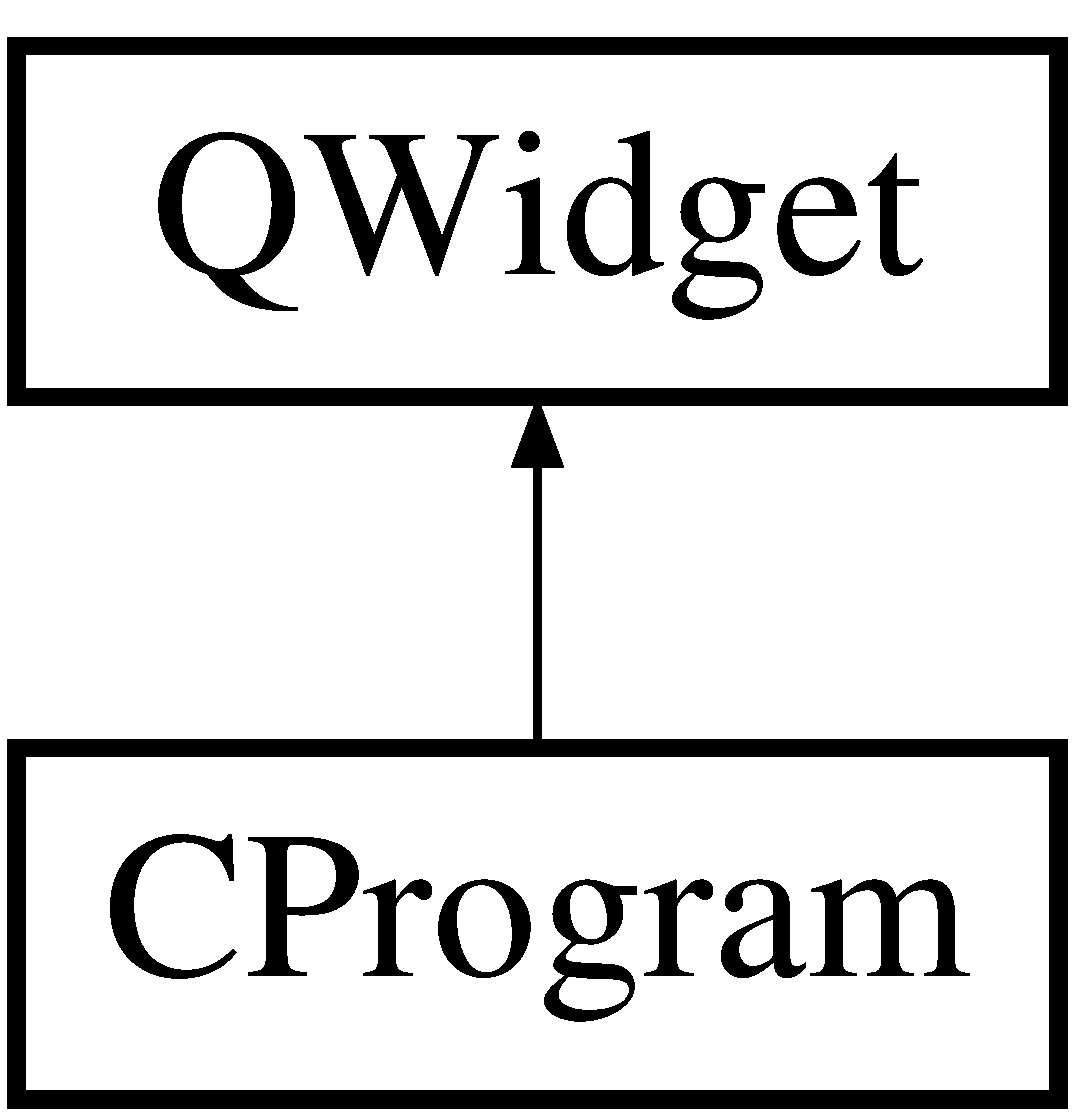
\includegraphics[height=2.000000cm]{class_c_program}
\end{center}
\end{figure}
\subsection*{Public Slots}
\begin{DoxyCompactItemize}
\item 
void \mbox{\hyperlink{class_c_program_a643bd73f256632b72a7d6182e8e7d807}{step}} ()
\begin{DoxyCompactList}\small\item\em W każdym kroku wywoływana jest funkcja update() dla wszystkich obiektów logicznych na mapie, następnie dla wszystkich obiektów graficznych wywoływana jest funkcja advance(), na koniec każdego kroku losowo dodawane są do mapy obiekty różnego typu aby w programie cały czas coś się działo. \end{DoxyCompactList}\end{DoxyCompactItemize}
\subsection*{Public Member Functions}
\begin{DoxyCompactItemize}
\item 
\mbox{\hyperlink{class_c_program_a74d3ca01d5e8b892f37684254ae546ed}{C\+Program}} ()
\begin{DoxyCompactList}\small\item\em Konstruktor programu tworzy scenę oraz widok, ustawia ich paramtery oraz tworzy mapę, a następnie inicjalizuje timer wywołujący co pewien okres czasu funkcję \mbox{\hyperlink{class_c_program_a643bd73f256632b72a7d6182e8e7d807}{step()}} \end{DoxyCompactList}\end{DoxyCompactItemize}


\subsection{Detailed Description}
Klasa zarządzająca działaniem programu. 

\subsection{Constructor \& Destructor Documentation}
\mbox{\Hypertarget{class_c_program_a74d3ca01d5e8b892f37684254ae546ed}\label{class_c_program_a74d3ca01d5e8b892f37684254ae546ed}} 
\index{C\+Program@{C\+Program}!C\+Program@{C\+Program}}
\index{C\+Program@{C\+Program}!C\+Program@{C\+Program}}
\subsubsection{\texorpdfstring{C\+Program()}{CProgram()}}
{\footnotesize\ttfamily C\+Program\+::\+C\+Program (\begin{DoxyParamCaption}{ }\end{DoxyParamCaption})}



Konstruktor programu tworzy scenę oraz widok, ustawia ich paramtery oraz tworzy mapę, a następnie inicjalizuje timer wywołujący co pewien okres czasu funkcję \mbox{\hyperlink{class_c_program_a643bd73f256632b72a7d6182e8e7d807}{step()}} 



\subsection{Member Function Documentation}
\mbox{\Hypertarget{class_c_program_a643bd73f256632b72a7d6182e8e7d807}\label{class_c_program_a643bd73f256632b72a7d6182e8e7d807}} 
\index{C\+Program@{C\+Program}!step@{step}}
\index{step@{step}!C\+Program@{C\+Program}}
\subsubsection{\texorpdfstring{step}{step}}
{\footnotesize\ttfamily void C\+Program\+::step (\begin{DoxyParamCaption}{ }\end{DoxyParamCaption})\hspace{0.3cm}{\ttfamily [slot]}}



W każdym kroku wywoływana jest funkcja update() dla wszystkich obiektów logicznych na mapie, następnie dla wszystkich obiektów graficznych wywoływana jest funkcja advance(), na koniec każdego kroku losowo dodawane są do mapy obiekty różnego typu aby w programie cały czas coś się działo. 



The documentation for this class was generated from the following files\+:\begin{DoxyCompactItemize}
\item 
\mbox{\hyperlink{cprogram_8h}{cprogram.\+h}}\item 
\mbox{\hyperlink{cprogram_8cpp}{cprogram.\+cpp}}\end{DoxyCompactItemize}

\hypertarget{class_c_robot}{}\section{C\+Robot Class Reference}
\label{class_c_robot}\index{C\+Robot@{C\+Robot}}


Klasa reprezentująca robota.  




{\ttfamily \#include $<$crobot.\+h$>$}

Inheritance diagram for C\+Robot\+:\begin{figure}[H]
\begin{center}
\leavevmode
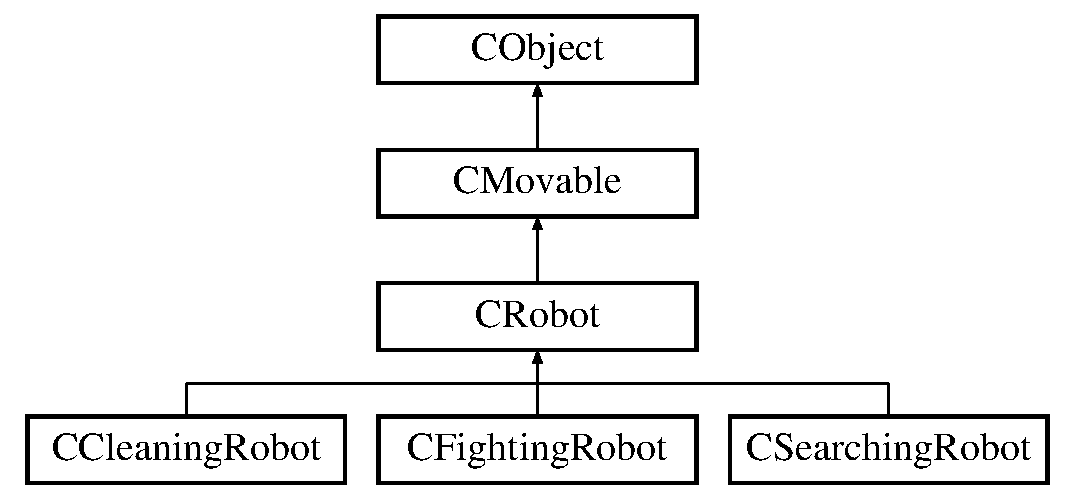
\includegraphics[height=4.000000cm]{class_c_robot}
\end{center}
\end{figure}
\subsection*{Public Member Functions}
\begin{DoxyCompactItemize}
\item 
\mbox{\hyperlink{class_c_robot_a9769daad02498cf1d6c7f91b9ed27ff5}{C\+Robot}} (\mbox{\hyperlink{class_c_map}{C\+Map}} $\ast$m)
\begin{DoxyCompactList}\small\item\em Umieszcza robota na mapie w losowym miejscu z losowymi parametrami. \end{DoxyCompactList}\item 
\mbox{\hyperlink{class_c_robot_a9efdb5f31b4380e2aff141e6c55f8515}{C\+Robot}} (qreal xv, qreal yv, \mbox{\hyperlink{class_c_map}{C\+Map}} $\ast$m)
\begin{DoxyCompactList}\small\item\em Umieszcza robota w konrektnym miejscu z losowymi parametrami. \end{DoxyCompactList}\item 
\mbox{\hyperlink{class_c_robot_a39050adcb2119ac8b3bd7042704b487a}{C\+Robot}} (qreal xv, qreal yv, qreal anglev, qreal rangev, \mbox{\hyperlink{class_c_map}{C\+Map}} $\ast$m)
\begin{DoxyCompactList}\small\item\em Umieszcza robota w konkretnym miejscu z konkretnymi parametrami. \end{DoxyCompactList}\item 
virtual void \mbox{\hyperlink{class_c_robot_a8ad8d55a840ced20f85a2a045e9e24ef}{update}} ()=0
\begin{DoxyCompactList}\small\item\em Funkcja wywoływana przy każdym kroku programu dla wszystkich obiektów, oddziaływuje na otoczenie oraz podejmuje decyzje na podstawie tego otoczenia, implementacja jest różna dla każdej z podklas na najniższym szczeblu hierarchii dziedziczenia. \end{DoxyCompactList}\item 
virtual void \mbox{\hyperlink{class_c_robot_a1de9be879213eadf7ded27caedb84598}{move}} ()=0
\begin{DoxyCompactList}\small\item\em Funkcja zmieniająca położenie obiektu przy każdym kroku; implementacja zależy od typu obieku. \end{DoxyCompactList}\item 
void \mbox{\hyperlink{class_c_robot_a5d173b8f2c8fae09df01a8f1fc9211fb}{add\+Item}} (\mbox{\hyperlink{class_c_non_movable}{C\+Non\+Movable}} $\ast$item)
\begin{DoxyCompactList}\small\item\em Funkcja dodająca nieruchomy obiekt do listy obiektów przechowywanych przez robota. \end{DoxyCompactList}\item 
void \mbox{\hyperlink{class_c_robot_a9a819529f710ae6d9dc376c78e6c5657}{move\+Randomly}} ()
\begin{DoxyCompactList}\small\item\em Funkcja zmieniająca położenie robota o jego prędkość w kierunku określonym przez orientację; losowo zmienia kąt o niewielką wartość, aby roboty nie jeździły cały czas po prostej. \end{DoxyCompactList}\item 
void \mbox{\hyperlink{class_c_robot_adc5f5ff12284e09613bae149ed8ded2c}{return\+To\+Map}} ()
\begin{DoxyCompactList}\small\item\em Funkcja, która obraca robota tak, aby wrócił on na planszę \end{DoxyCompactList}\item 
void \mbox{\hyperlink{class_c_robot_a9bab21d24d736824d37283811abfb5fd}{go\+To}} (\mbox{\hyperlink{class_c_object}{C\+Object}} $\ast$o)
\begin{DoxyCompactList}\small\item\em Robot porusza się tak, aby zbliżyć się do podanego obiektu. \end{DoxyCompactList}\item 
void \mbox{\hyperlink{class_c_robot_ae667593c574d4ec859de15d5ae7e7c22}{avoid}} (std\+::vector$<$ \mbox{\hyperlink{class_c_non_movable}{C\+Non\+Movable}} $\ast$$>$ o, std\+::vector$<$ \mbox{\hyperlink{class_c_robot}{C\+Robot}} $\ast$$>$ r, std\+::vector$<$ \mbox{\hyperlink{class_c_obstacle}{C\+Obstacle}} $\ast$$>$ ob)
\begin{DoxyCompactList}\small\item\em Robot porusza się tak, aby oddalić się od podanych obiektów i uniknąć zderzeń z nimi. \end{DoxyCompactList}\end{DoxyCompactItemize}
\subsection*{Protected Attributes}
\begin{DoxyCompactItemize}
\item 
std\+::vector$<$ \mbox{\hyperlink{class_c_non_movable}{C\+Non\+Movable}} $\ast$ $>$ \mbox{\hyperlink{class_c_robot_a8f676285c6d121ae209047b467c48947}{items}}
\begin{DoxyCompactList}\small\item\em Lista nieruchomych obiektów zebranych przez robota. \end{DoxyCompactList}\end{DoxyCompactItemize}


\subsection{Detailed Description}
Klasa reprezentująca robota. 

\subsection{Constructor \& Destructor Documentation}
\mbox{\Hypertarget{class_c_robot_a9769daad02498cf1d6c7f91b9ed27ff5}\label{class_c_robot_a9769daad02498cf1d6c7f91b9ed27ff5}} 
\index{C\+Robot@{C\+Robot}!C\+Robot@{C\+Robot}}
\index{C\+Robot@{C\+Robot}!C\+Robot@{C\+Robot}}
\subsubsection{\texorpdfstring{C\+Robot()}{CRobot()}\hspace{0.1cm}{\footnotesize\ttfamily [1/3]}}
{\footnotesize\ttfamily C\+Robot\+::\+C\+Robot (\begin{DoxyParamCaption}\item[{\mbox{\hyperlink{class_c_map}{C\+Map}} $\ast$}]{m }\end{DoxyParamCaption})}



Umieszcza robota na mapie w losowym miejscu z losowymi parametrami. 

\mbox{\Hypertarget{class_c_robot_a9efdb5f31b4380e2aff141e6c55f8515}\label{class_c_robot_a9efdb5f31b4380e2aff141e6c55f8515}} 
\index{C\+Robot@{C\+Robot}!C\+Robot@{C\+Robot}}
\index{C\+Robot@{C\+Robot}!C\+Robot@{C\+Robot}}
\subsubsection{\texorpdfstring{C\+Robot()}{CRobot()}\hspace{0.1cm}{\footnotesize\ttfamily [2/3]}}
{\footnotesize\ttfamily C\+Robot\+::\+C\+Robot (\begin{DoxyParamCaption}\item[{qreal}]{xv,  }\item[{qreal}]{yv,  }\item[{\mbox{\hyperlink{class_c_map}{C\+Map}} $\ast$}]{m }\end{DoxyParamCaption})}



Umieszcza robota w konrektnym miejscu z losowymi parametrami. 


\begin{DoxyParams}{Parameters}
{\em xv} & Współrzędna x \\
\hline
{\em yv} & Współrzędna y \\
\hline
\end{DoxyParams}
\mbox{\Hypertarget{class_c_robot_a39050adcb2119ac8b3bd7042704b487a}\label{class_c_robot_a39050adcb2119ac8b3bd7042704b487a}} 
\index{C\+Robot@{C\+Robot}!C\+Robot@{C\+Robot}}
\index{C\+Robot@{C\+Robot}!C\+Robot@{C\+Robot}}
\subsubsection{\texorpdfstring{C\+Robot()}{CRobot()}\hspace{0.1cm}{\footnotesize\ttfamily [3/3]}}
{\footnotesize\ttfamily C\+Robot\+::\+C\+Robot (\begin{DoxyParamCaption}\item[{qreal}]{xv,  }\item[{qreal}]{yv,  }\item[{qreal}]{anglev,  }\item[{qreal}]{rangev,  }\item[{\mbox{\hyperlink{class_c_map}{C\+Map}} $\ast$}]{m }\end{DoxyParamCaption})}



Umieszcza robota w konkretnym miejscu z konkretnymi parametrami. 


\begin{DoxyParams}{Parameters}
{\em xv} & Współrzędna x \\
\hline
{\em yv} & Współrzędna y \\
\hline
{\em anglev} & Orientacja \\
\hline
{\em rangev} & Zasięg \\
\hline
\end{DoxyParams}


\subsection{Member Function Documentation}
\mbox{\Hypertarget{class_c_robot_a5d173b8f2c8fae09df01a8f1fc9211fb}\label{class_c_robot_a5d173b8f2c8fae09df01a8f1fc9211fb}} 
\index{C\+Robot@{C\+Robot}!add\+Item@{add\+Item}}
\index{add\+Item@{add\+Item}!C\+Robot@{C\+Robot}}
\subsubsection{\texorpdfstring{add\+Item()}{addItem()}}
{\footnotesize\ttfamily void C\+Robot\+::add\+Item (\begin{DoxyParamCaption}\item[{\mbox{\hyperlink{class_c_non_movable}{C\+Non\+Movable}} $\ast$}]{item }\end{DoxyParamCaption})}



Funkcja dodająca nieruchomy obiekt do listy obiektów przechowywanych przez robota. 


\begin{DoxyParams}{Parameters}
{\em item} & Obiekt, który jest dodawany \\
\hline
\end{DoxyParams}
\mbox{\Hypertarget{class_c_robot_ae667593c574d4ec859de15d5ae7e7c22}\label{class_c_robot_ae667593c574d4ec859de15d5ae7e7c22}} 
\index{C\+Robot@{C\+Robot}!avoid@{avoid}}
\index{avoid@{avoid}!C\+Robot@{C\+Robot}}
\subsubsection{\texorpdfstring{avoid()}{avoid()}}
{\footnotesize\ttfamily void C\+Robot\+::avoid (\begin{DoxyParamCaption}\item[{std\+::vector$<$ \mbox{\hyperlink{class_c_non_movable}{C\+Non\+Movable}} $\ast$$>$}]{o,  }\item[{std\+::vector$<$ \mbox{\hyperlink{class_c_robot}{C\+Robot}} $\ast$$>$}]{r,  }\item[{std\+::vector$<$ \mbox{\hyperlink{class_c_obstacle}{C\+Obstacle}} $\ast$$>$}]{ob }\end{DoxyParamCaption})}



Robot porusza się tak, aby oddalić się od podanych obiektów i uniknąć zderzeń z nimi. 


\begin{DoxyParams}{Parameters}
{\em o} & Nieruchome obiekty, które należy omijać \\
\hline
{\em r} & Roboty, które należy omijać lub przepuszczać \\
\hline
{\em ob} & Przeszkody, które należy omijać lub przepuszczać \\
\hline
\end{DoxyParams}
\mbox{\Hypertarget{class_c_robot_a9bab21d24d736824d37283811abfb5fd}\label{class_c_robot_a9bab21d24d736824d37283811abfb5fd}} 
\index{C\+Robot@{C\+Robot}!go\+To@{go\+To}}
\index{go\+To@{go\+To}!C\+Robot@{C\+Robot}}
\subsubsection{\texorpdfstring{go\+To()}{goTo()}}
{\footnotesize\ttfamily void C\+Robot\+::go\+To (\begin{DoxyParamCaption}\item[{\mbox{\hyperlink{class_c_object}{C\+Object}} $\ast$}]{o }\end{DoxyParamCaption})}



Robot porusza się tak, aby zbliżyć się do podanego obiektu. 


\begin{DoxyParams}{Parameters}
{\em o} & Obiekt, w którego kierunku robot ma się poruszać \\
\hline
\end{DoxyParams}
\mbox{\Hypertarget{class_c_robot_a1de9be879213eadf7ded27caedb84598}\label{class_c_robot_a1de9be879213eadf7ded27caedb84598}} 
\index{C\+Robot@{C\+Robot}!move@{move}}
\index{move@{move}!C\+Robot@{C\+Robot}}
\subsubsection{\texorpdfstring{move()}{move()}}
{\footnotesize\ttfamily virtual void C\+Robot\+::move (\begin{DoxyParamCaption}{ }\end{DoxyParamCaption})\hspace{0.3cm}{\ttfamily [pure virtual]}}



Funkcja zmieniająca położenie obiektu przy każdym kroku; implementacja zależy od typu obieku. 



Implements \mbox{\hyperlink{class_c_movable_a8e66e106f13362d24462ce0c9d0431af}{C\+Movable}}.



Implemented in \mbox{\hyperlink{class_c_cleaning_robot_a1ad227a5f3508a8e78fcecae7d3de53b}{C\+Cleaning\+Robot}}, \mbox{\hyperlink{class_c_searching_robot_a2c2150e7fd1cefbb5851e039cd76572f}{C\+Searching\+Robot}}, and \mbox{\hyperlink{class_c_fighting_robot_af644acbba178e256566e9dbd230aa4db}{C\+Fighting\+Robot}}.

\mbox{\Hypertarget{class_c_robot_a9a819529f710ae6d9dc376c78e6c5657}\label{class_c_robot_a9a819529f710ae6d9dc376c78e6c5657}} 
\index{C\+Robot@{C\+Robot}!move\+Randomly@{move\+Randomly}}
\index{move\+Randomly@{move\+Randomly}!C\+Robot@{C\+Robot}}
\subsubsection{\texorpdfstring{move\+Randomly()}{moveRandomly()}}
{\footnotesize\ttfamily void C\+Robot\+::move\+Randomly (\begin{DoxyParamCaption}{ }\end{DoxyParamCaption})}



Funkcja zmieniająca położenie robota o jego prędkość w kierunku określonym przez orientację; losowo zmienia kąt o niewielką wartość, aby roboty nie jeździły cały czas po prostej. 

\mbox{\Hypertarget{class_c_robot_adc5f5ff12284e09613bae149ed8ded2c}\label{class_c_robot_adc5f5ff12284e09613bae149ed8ded2c}} 
\index{C\+Robot@{C\+Robot}!return\+To\+Map@{return\+To\+Map}}
\index{return\+To\+Map@{return\+To\+Map}!C\+Robot@{C\+Robot}}
\subsubsection{\texorpdfstring{return\+To\+Map()}{returnToMap()}}
{\footnotesize\ttfamily void C\+Robot\+::return\+To\+Map (\begin{DoxyParamCaption}{ }\end{DoxyParamCaption})}



Funkcja, która obraca robota tak, aby wrócił on na planszę 

\mbox{\Hypertarget{class_c_robot_a8ad8d55a840ced20f85a2a045e9e24ef}\label{class_c_robot_a8ad8d55a840ced20f85a2a045e9e24ef}} 
\index{C\+Robot@{C\+Robot}!update@{update}}
\index{update@{update}!C\+Robot@{C\+Robot}}
\subsubsection{\texorpdfstring{update()}{update()}}
{\footnotesize\ttfamily virtual void C\+Robot\+::update (\begin{DoxyParamCaption}{ }\end{DoxyParamCaption})\hspace{0.3cm}{\ttfamily [pure virtual]}}



Funkcja wywoływana przy każdym kroku programu dla wszystkich obiektów, oddziaływuje na otoczenie oraz podejmuje decyzje na podstawie tego otoczenia, implementacja jest różna dla każdej z podklas na najniższym szczeblu hierarchii dziedziczenia. 



Implements \mbox{\hyperlink{class_c_movable_af45fc62960d86ef62949d078141e9d62}{C\+Movable}}.



Implemented in \mbox{\hyperlink{class_c_cleaning_robot_afd8b3a58abfc91ebdce32af3686c5e9f}{C\+Cleaning\+Robot}}, \mbox{\hyperlink{class_c_searching_robot_a6e9cdc9eccd32a470d8953f1a3cccd46}{C\+Searching\+Robot}}, and \mbox{\hyperlink{class_c_fighting_robot_a3ae0ea383f809766e53c81348a07daaa}{C\+Fighting\+Robot}}.



\subsection{Member Data Documentation}
\mbox{\Hypertarget{class_c_robot_a8f676285c6d121ae209047b467c48947}\label{class_c_robot_a8f676285c6d121ae209047b467c48947}} 
\index{C\+Robot@{C\+Robot}!items@{items}}
\index{items@{items}!C\+Robot@{C\+Robot}}
\subsubsection{\texorpdfstring{items}{items}}
{\footnotesize\ttfamily std\+::vector$<$\mbox{\hyperlink{class_c_non_movable}{C\+Non\+Movable}}$\ast$$>$ C\+Robot\+::items\hspace{0.3cm}{\ttfamily [protected]}}



Lista nieruchomych obiektów zebranych przez robota. 



The documentation for this class was generated from the following files\+:\begin{DoxyCompactItemize}
\item 
\mbox{\hyperlink{crobot_8h}{crobot.\+h}}\item 
\mbox{\hyperlink{crobot_8cpp}{crobot.\+cpp}}\end{DoxyCompactItemize}

\hypertarget{class_c_searching_robot}{}\section{C\+Searching\+Robot Class Reference}
\label{class_c_searching_robot}\index{C\+Searching\+Robot@{C\+Searching\+Robot}}


Robot zajmujący się szukaniem skarbów.  




{\ttfamily \#include $<$csearchingrobot.\+h$>$}

Inheritance diagram for C\+Searching\+Robot\+:\begin{figure}[H]
\begin{center}
\leavevmode
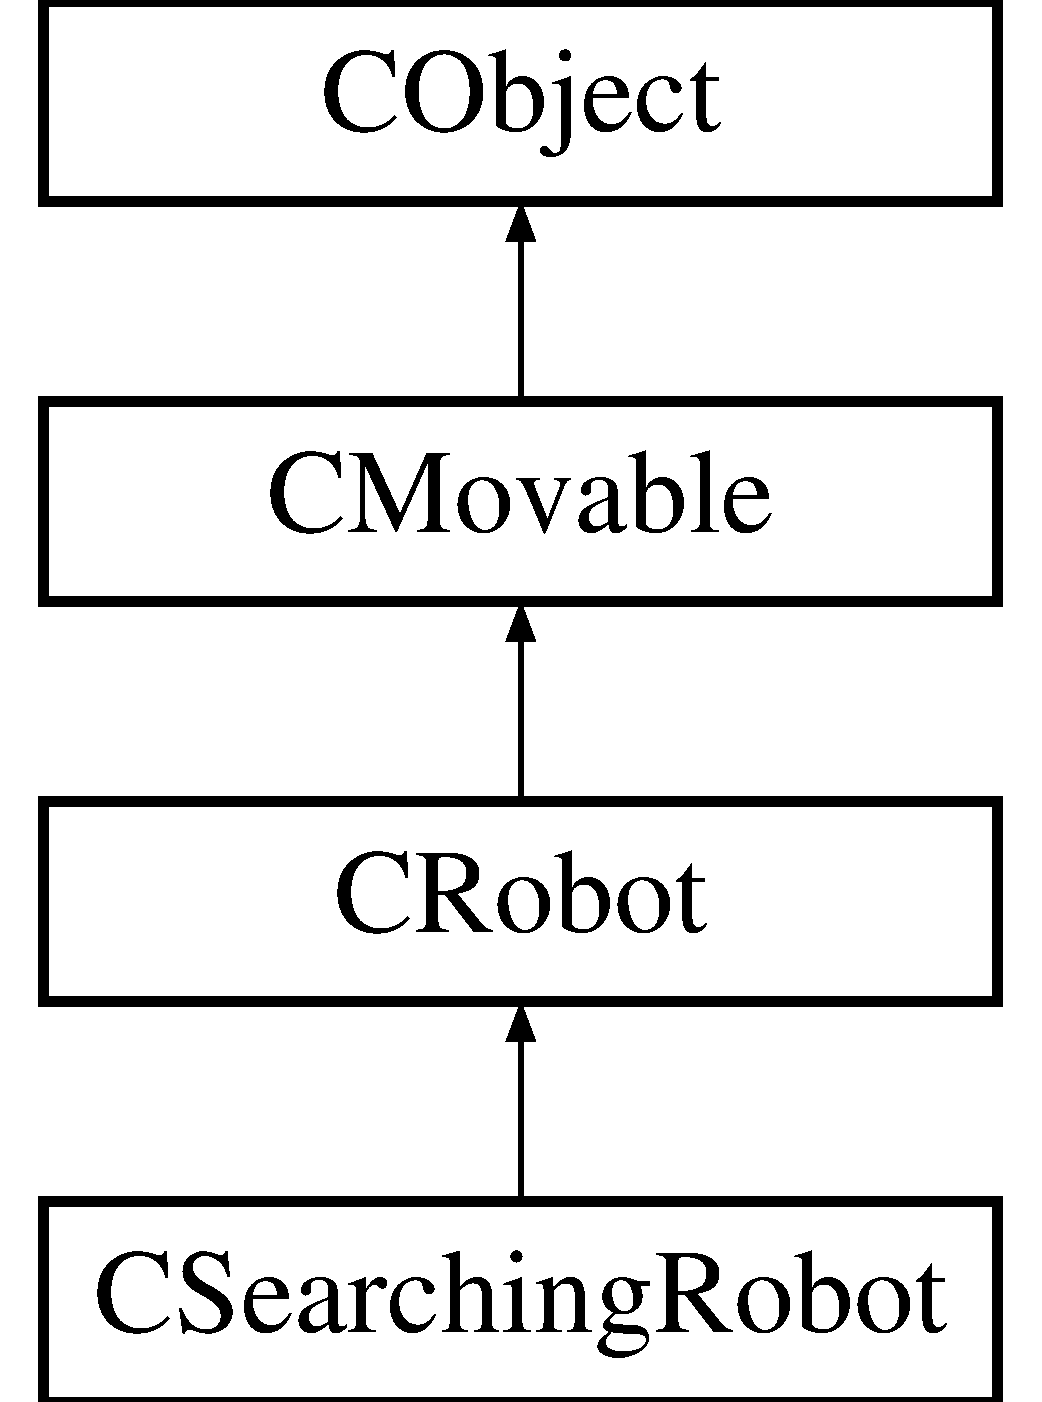
\includegraphics[height=4.000000cm]{class_c_searching_robot}
\end{center}
\end{figure}
\subsection*{Public Member Functions}
\begin{DoxyCompactItemize}
\item 
\mbox{\hyperlink{class_c_searching_robot_a94c25b4cc475f118b8d6521b169a3b09}{C\+Searching\+Robot}} (\mbox{\hyperlink{class_c_map}{C\+Map}} $\ast$m)
\item 
\mbox{\hyperlink{class_c_searching_robot_a4b9874d7d35fabecc7953bf31ab18fc1}{C\+Searching\+Robot}} (qreal xv, qreal yv, \mbox{\hyperlink{class_c_map}{C\+Map}} $\ast$m)
\item 
\mbox{\hyperlink{class_c_searching_robot_a89fb6d088efb21dfa85395c587f0e12d}{C\+Searching\+Robot}} (qreal xv, qreal yv, qreal anglev, qreal rangev, \mbox{\hyperlink{class_c_map}{C\+Map}} $\ast$m)
\item 
virtual \mbox{\hyperlink{class_c_searching_robot_aaa18ea94f4bd833465f9801faef6bd75}{$\sim$\+C\+Searching\+Robot}} ()
\item 
void \mbox{\hyperlink{class_c_searching_robot_a2c2150e7fd1cefbb5851e039cd76572f}{move}} ()
\begin{DoxyCompactList}\small\item\em Funkcja stara się w pierwszej kolejności uniknąć kolizji z innymi obiektami; jeśli nie wystąpi kolizja, sprawdzane jest, czy robot jest na mapie; jeśli nie jest na mapie, próbuje wrócić i kończy ruch; w przeciwnym wypadku kieruje się w stronę najbliższego skarbu, o ile jakieś są w zasięgu; jeśli w pobliżu nie ma żadnych brudów, robot porusza się losowo. \end{DoxyCompactList}\item 
void \mbox{\hyperlink{class_c_searching_robot_a6e9cdc9eccd32a470d8953f1a3cccd46}{update}} ()
\begin{DoxyCompactList}\small\item\em Funkcja sprawdza, czy występują kolizje z jakimiś skarbami i zbiera ewentualne kolidujące skarby; następnie wywoływana jest funkcja \mbox{\hyperlink{class_c_searching_robot_a2c2150e7fd1cefbb5851e039cd76572f}{move()}} \end{DoxyCompactList}\item 
void \mbox{\hyperlink{class_c_searching_robot_a1f09a0003c1c7c309895745a2dbad885}{collect}} (\mbox{\hyperlink{class_c_treasure}{C\+Treasure}} $\ast$treasure)
\begin{DoxyCompactList}\small\item\em Funkcja dodająca do listy zebranych obiektów podany skarb. \end{DoxyCompactList}\end{DoxyCompactItemize}
\subsection*{Additional Inherited Members}


\subsection{Detailed Description}
Robot zajmujący się szukaniem skarbów. 

\subsection{Constructor \& Destructor Documentation}
\mbox{\Hypertarget{class_c_searching_robot_a94c25b4cc475f118b8d6521b169a3b09}\label{class_c_searching_robot_a94c25b4cc475f118b8d6521b169a3b09}} 
\index{C\+Searching\+Robot@{C\+Searching\+Robot}!C\+Searching\+Robot@{C\+Searching\+Robot}}
\index{C\+Searching\+Robot@{C\+Searching\+Robot}!C\+Searching\+Robot@{C\+Searching\+Robot}}
\subsubsection{\texorpdfstring{C\+Searching\+Robot()}{CSearchingRobot()}\hspace{0.1cm}{\footnotesize\ttfamily [1/3]}}
{\footnotesize\ttfamily C\+Searching\+Robot\+::\+C\+Searching\+Robot (\begin{DoxyParamCaption}\item[{\mbox{\hyperlink{class_c_map}{C\+Map}} $\ast$}]{m }\end{DoxyParamCaption})}

\mbox{\Hypertarget{class_c_searching_robot_a4b9874d7d35fabecc7953bf31ab18fc1}\label{class_c_searching_robot_a4b9874d7d35fabecc7953bf31ab18fc1}} 
\index{C\+Searching\+Robot@{C\+Searching\+Robot}!C\+Searching\+Robot@{C\+Searching\+Robot}}
\index{C\+Searching\+Robot@{C\+Searching\+Robot}!C\+Searching\+Robot@{C\+Searching\+Robot}}
\subsubsection{\texorpdfstring{C\+Searching\+Robot()}{CSearchingRobot()}\hspace{0.1cm}{\footnotesize\ttfamily [2/3]}}
{\footnotesize\ttfamily C\+Searching\+Robot\+::\+C\+Searching\+Robot (\begin{DoxyParamCaption}\item[{qreal}]{xv,  }\item[{qreal}]{yv,  }\item[{\mbox{\hyperlink{class_c_map}{C\+Map}} $\ast$}]{m }\end{DoxyParamCaption})}

\mbox{\Hypertarget{class_c_searching_robot_a89fb6d088efb21dfa85395c587f0e12d}\label{class_c_searching_robot_a89fb6d088efb21dfa85395c587f0e12d}} 
\index{C\+Searching\+Robot@{C\+Searching\+Robot}!C\+Searching\+Robot@{C\+Searching\+Robot}}
\index{C\+Searching\+Robot@{C\+Searching\+Robot}!C\+Searching\+Robot@{C\+Searching\+Robot}}
\subsubsection{\texorpdfstring{C\+Searching\+Robot()}{CSearchingRobot()}\hspace{0.1cm}{\footnotesize\ttfamily [3/3]}}
{\footnotesize\ttfamily C\+Searching\+Robot\+::\+C\+Searching\+Robot (\begin{DoxyParamCaption}\item[{qreal}]{xv,  }\item[{qreal}]{yv,  }\item[{qreal}]{anglev,  }\item[{qreal}]{rangev,  }\item[{\mbox{\hyperlink{class_c_map}{C\+Map}} $\ast$}]{m }\end{DoxyParamCaption})}

\mbox{\Hypertarget{class_c_searching_robot_aaa18ea94f4bd833465f9801faef6bd75}\label{class_c_searching_robot_aaa18ea94f4bd833465f9801faef6bd75}} 
\index{C\+Searching\+Robot@{C\+Searching\+Robot}!````~C\+Searching\+Robot@{$\sim$\+C\+Searching\+Robot}}
\index{````~C\+Searching\+Robot@{$\sim$\+C\+Searching\+Robot}!C\+Searching\+Robot@{C\+Searching\+Robot}}
\subsubsection{\texorpdfstring{$\sim$\+C\+Searching\+Robot()}{~CSearchingRobot()}}
{\footnotesize\ttfamily C\+Searching\+Robot\+::$\sim$\+C\+Searching\+Robot (\begin{DoxyParamCaption}{ }\end{DoxyParamCaption})\hspace{0.3cm}{\ttfamily [virtual]}}



\subsection{Member Function Documentation}
\mbox{\Hypertarget{class_c_searching_robot_a1f09a0003c1c7c309895745a2dbad885}\label{class_c_searching_robot_a1f09a0003c1c7c309895745a2dbad885}} 
\index{C\+Searching\+Robot@{C\+Searching\+Robot}!collect@{collect}}
\index{collect@{collect}!C\+Searching\+Robot@{C\+Searching\+Robot}}
\subsubsection{\texorpdfstring{collect()}{collect()}}
{\footnotesize\ttfamily void C\+Searching\+Robot\+::collect (\begin{DoxyParamCaption}\item[{\mbox{\hyperlink{class_c_treasure}{C\+Treasure}} $\ast$}]{treasure }\end{DoxyParamCaption})}



Funkcja dodająca do listy zebranych obiektów podany skarb. 


\begin{DoxyParams}{Parameters}
{\em treasure} & Skarb, który należy zebrać \\
\hline
\end{DoxyParams}
\mbox{\Hypertarget{class_c_searching_robot_a2c2150e7fd1cefbb5851e039cd76572f}\label{class_c_searching_robot_a2c2150e7fd1cefbb5851e039cd76572f}} 
\index{C\+Searching\+Robot@{C\+Searching\+Robot}!move@{move}}
\index{move@{move}!C\+Searching\+Robot@{C\+Searching\+Robot}}
\subsubsection{\texorpdfstring{move()}{move()}}
{\footnotesize\ttfamily void C\+Searching\+Robot\+::move (\begin{DoxyParamCaption}{ }\end{DoxyParamCaption})\hspace{0.3cm}{\ttfamily [virtual]}}



Funkcja stara się w pierwszej kolejności uniknąć kolizji z innymi obiektami; jeśli nie wystąpi kolizja, sprawdzane jest, czy robot jest na mapie; jeśli nie jest na mapie, próbuje wrócić i kończy ruch; w przeciwnym wypadku kieruje się w stronę najbliższego skarbu, o ile jakieś są w zasięgu; jeśli w pobliżu nie ma żadnych brudów, robot porusza się losowo. 



Implements \mbox{\hyperlink{class_c_robot_a1de9be879213eadf7ded27caedb84598}{C\+Robot}}.

\mbox{\Hypertarget{class_c_searching_robot_a6e9cdc9eccd32a470d8953f1a3cccd46}\label{class_c_searching_robot_a6e9cdc9eccd32a470d8953f1a3cccd46}} 
\index{C\+Searching\+Robot@{C\+Searching\+Robot}!update@{update}}
\index{update@{update}!C\+Searching\+Robot@{C\+Searching\+Robot}}
\subsubsection{\texorpdfstring{update()}{update()}}
{\footnotesize\ttfamily void C\+Searching\+Robot\+::update (\begin{DoxyParamCaption}{ }\end{DoxyParamCaption})\hspace{0.3cm}{\ttfamily [virtual]}}



Funkcja sprawdza, czy występują kolizje z jakimiś skarbami i zbiera ewentualne kolidujące skarby; następnie wywoływana jest funkcja \mbox{\hyperlink{class_c_searching_robot_a2c2150e7fd1cefbb5851e039cd76572f}{move()}} 



Implements \mbox{\hyperlink{class_c_robot_a8ad8d55a840ced20f85a2a045e9e24ef}{C\+Robot}}.



The documentation for this class was generated from the following files\+:\begin{DoxyCompactItemize}
\item 
\mbox{\hyperlink{csearchingrobot_8h}{csearchingrobot.\+h}}\item 
\mbox{\hyperlink{csearchingrobot_8cpp}{csearchingrobot.\+cpp}}\end{DoxyCompactItemize}

\hypertarget{class_c_treasure}{}\section{C\+Treasure Class Reference}
\label{class_c_treasure}\index{C\+Treasure@{C\+Treasure}}


Obiekty zbierane przez roboty zajmujące się ich szukaniem.  




{\ttfamily \#include $<$ctreasure.\+h$>$}

Inheritance diagram for C\+Treasure\+:\begin{figure}[H]
\begin{center}
\leavevmode
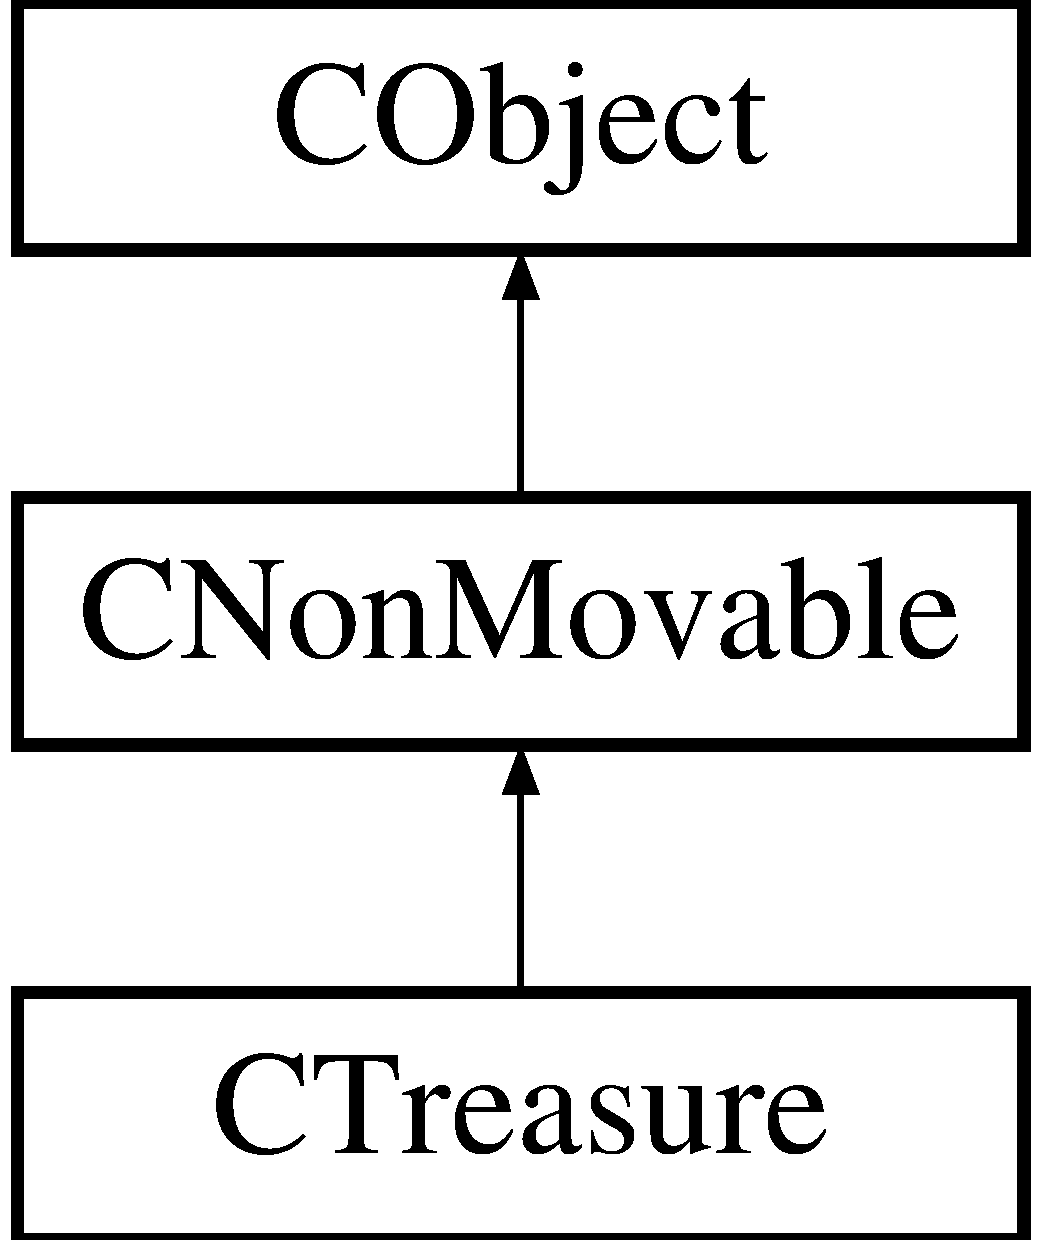
\includegraphics[height=3.000000cm]{class_c_treasure}
\end{center}
\end{figure}
\subsection*{Public Member Functions}
\begin{DoxyCompactItemize}
\item 
\mbox{\hyperlink{class_c_treasure_aeb12f1d0197b6be908d30c5a36596a17}{C\+Treasure}} (\mbox{\hyperlink{class_c_map}{C\+Map}} $\ast$m)
\item 
virtual \mbox{\hyperlink{class_c_treasure_ad8197def05d5e5583f71a9d5e4ed8161}{$\sim$\+C\+Treasure}} ()
\item 
void \mbox{\hyperlink{class_c_treasure_a5030f2a7279aa608c40741f9e7040a90}{update}} ()
\begin{DoxyCompactList}\small\item\em Wartość skarbu wraz z upływem czasu maleje. \end{DoxyCompactList}\item 
void \mbox{\hyperlink{class_c_treasure_a00a58d2aea1c7844e502c8bcb3576678}{get\+Collected}} ()
\begin{DoxyCompactList}\small\item\em Funkcja usuwająca obiekt z mapy. \end{DoxyCompactList}\end{DoxyCompactItemize}
\subsection*{Additional Inherited Members}


\subsection{Detailed Description}
Obiekty zbierane przez roboty zajmujące się ich szukaniem. 

\subsection{Constructor \& Destructor Documentation}
\mbox{\Hypertarget{class_c_treasure_aeb12f1d0197b6be908d30c5a36596a17}\label{class_c_treasure_aeb12f1d0197b6be908d30c5a36596a17}} 
\index{C\+Treasure@{C\+Treasure}!C\+Treasure@{C\+Treasure}}
\index{C\+Treasure@{C\+Treasure}!C\+Treasure@{C\+Treasure}}
\subsubsection{\texorpdfstring{C\+Treasure()}{CTreasure()}}
{\footnotesize\ttfamily C\+Treasure\+::\+C\+Treasure (\begin{DoxyParamCaption}\item[{\mbox{\hyperlink{class_c_map}{C\+Map}} $\ast$}]{m }\end{DoxyParamCaption})}

\mbox{\Hypertarget{class_c_treasure_ad8197def05d5e5583f71a9d5e4ed8161}\label{class_c_treasure_ad8197def05d5e5583f71a9d5e4ed8161}} 
\index{C\+Treasure@{C\+Treasure}!````~C\+Treasure@{$\sim$\+C\+Treasure}}
\index{````~C\+Treasure@{$\sim$\+C\+Treasure}!C\+Treasure@{C\+Treasure}}
\subsubsection{\texorpdfstring{$\sim$\+C\+Treasure()}{~CTreasure()}}
{\footnotesize\ttfamily C\+Treasure\+::$\sim$\+C\+Treasure (\begin{DoxyParamCaption}{ }\end{DoxyParamCaption})\hspace{0.3cm}{\ttfamily [virtual]}}



\subsection{Member Function Documentation}
\mbox{\Hypertarget{class_c_treasure_a00a58d2aea1c7844e502c8bcb3576678}\label{class_c_treasure_a00a58d2aea1c7844e502c8bcb3576678}} 
\index{C\+Treasure@{C\+Treasure}!get\+Collected@{get\+Collected}}
\index{get\+Collected@{get\+Collected}!C\+Treasure@{C\+Treasure}}
\subsubsection{\texorpdfstring{get\+Collected()}{getCollected()}}
{\footnotesize\ttfamily void C\+Treasure\+::get\+Collected (\begin{DoxyParamCaption}{ }\end{DoxyParamCaption})}



Funkcja usuwająca obiekt z mapy. 

\mbox{\Hypertarget{class_c_treasure_a5030f2a7279aa608c40741f9e7040a90}\label{class_c_treasure_a5030f2a7279aa608c40741f9e7040a90}} 
\index{C\+Treasure@{C\+Treasure}!update@{update}}
\index{update@{update}!C\+Treasure@{C\+Treasure}}
\subsubsection{\texorpdfstring{update()}{update()}}
{\footnotesize\ttfamily void C\+Treasure\+::update (\begin{DoxyParamCaption}{ }\end{DoxyParamCaption})\hspace{0.3cm}{\ttfamily [virtual]}}



Wartość skarbu wraz z upływem czasu maleje. 



Implements \mbox{\hyperlink{class_c_non_movable_ace03bea0246940c6c5c0b26ffa1ef165}{C\+Non\+Movable}}.



The documentation for this class was generated from the following files\+:\begin{DoxyCompactItemize}
\item 
\mbox{\hyperlink{ctreasure_8h}{ctreasure.\+h}}\item 
\mbox{\hyperlink{ctreasure_8cpp}{ctreasure.\+cpp}}\end{DoxyCompactItemize}

\chapter{File Documentation}
\hypertarget{cbullet_8cpp}{}\section{cbullet.\+cpp File Reference}
\label{cbullet_8cpp}\index{cbullet.\+cpp@{cbullet.\+cpp}}
{\ttfamily \#include \char`\"{}cbullet.\+h\char`\"{}}\newline
{\ttfamily \#include \char`\"{}cmap.\+h\char`\"{}}\newline

\hypertarget{cbullet_8h}{}\section{cbullet.\+h File Reference}
\label{cbullet_8h}\index{cbullet.\+h@{cbullet.\+h}}
{\ttfamily \#include \char`\"{}cmovable.\+h\char`\"{}}\newline
{\ttfamily \#include \char`\"{}cfightingrobot.\+h\char`\"{}}\newline
\subsection*{Classes}
\begin{DoxyCompactItemize}
\item 
class \mbox{\hyperlink{class_c_bullet}{C\+Bullet}}
\begin{DoxyCompactList}\small\item\em Pociski wystrzeliwywane przez roboty walczące. \end{DoxyCompactList}\end{DoxyCompactItemize}
\subsection*{Variables}
\begin{DoxyCompactItemize}
\item 
const int \mbox{\hyperlink{cbullet_8h_a2bb9465b72111b2aaa64551b7d929370}{bullet\+Speed}} = 30
\begin{DoxyCompactList}\small\item\em Stała określająca prędkość pocisku. \end{DoxyCompactList}\item 
const int \mbox{\hyperlink{cbullet_8h_a61f37da317cca96a9841d87517c29190}{bullet\+Lifetime}} = 4
\begin{DoxyCompactList}\small\item\em Stała określająca czas życia pocisku. \end{DoxyCompactList}\item 
const int \mbox{\hyperlink{cbullet_8h_a67da44a72756bb61a26f9f0f5c8c6c92}{bullet\+Size}} = 10
\begin{DoxyCompactList}\small\item\em Stała określająca wielkość pocisku. \end{DoxyCompactList}\end{DoxyCompactItemize}


\subsection{Variable Documentation}
\mbox{\Hypertarget{cbullet_8h_a61f37da317cca96a9841d87517c29190}\label{cbullet_8h_a61f37da317cca96a9841d87517c29190}} 
\index{cbullet.\+h@{cbullet.\+h}!bullet\+Lifetime@{bullet\+Lifetime}}
\index{bullet\+Lifetime@{bullet\+Lifetime}!cbullet.\+h@{cbullet.\+h}}
\subsubsection{\texorpdfstring{bullet\+Lifetime}{bulletLifetime}}
{\footnotesize\ttfamily const int bullet\+Lifetime = 4}



Stała określająca czas życia pocisku. 

\mbox{\Hypertarget{cbullet_8h_a67da44a72756bb61a26f9f0f5c8c6c92}\label{cbullet_8h_a67da44a72756bb61a26f9f0f5c8c6c92}} 
\index{cbullet.\+h@{cbullet.\+h}!bullet\+Size@{bullet\+Size}}
\index{bullet\+Size@{bullet\+Size}!cbullet.\+h@{cbullet.\+h}}
\subsubsection{\texorpdfstring{bullet\+Size}{bulletSize}}
{\footnotesize\ttfamily const int bullet\+Size = 10}



Stała określająca wielkość pocisku. 

\mbox{\Hypertarget{cbullet_8h_a2bb9465b72111b2aaa64551b7d929370}\label{cbullet_8h_a2bb9465b72111b2aaa64551b7d929370}} 
\index{cbullet.\+h@{cbullet.\+h}!bullet\+Speed@{bullet\+Speed}}
\index{bullet\+Speed@{bullet\+Speed}!cbullet.\+h@{cbullet.\+h}}
\subsubsection{\texorpdfstring{bullet\+Speed}{bulletSpeed}}
{\footnotesize\ttfamily const int bullet\+Speed = 30}



Stała określająca prędkość pocisku. 


\hypertarget{ccleaningrobot_8cpp}{}\section{ccleaningrobot.\+cpp File Reference}
\label{ccleaningrobot_8cpp}\index{ccleaningrobot.\+cpp@{ccleaningrobot.\+cpp}}
{\ttfamily \#include \char`\"{}ccleaningrobot.\+h\char`\"{}}\newline
{\ttfamily \#include $<$Q\+Random\+Generator$>$}\newline
{\ttfamily \#include \char`\"{}cmap.\+h\char`\"{}}\newline

\hypertarget{ccleaningrobot_8h}{}\section{ccleaningrobot.\+h File Reference}
\label{ccleaningrobot_8h}\index{ccleaningrobot.\+h@{ccleaningrobot.\+h}}
{\ttfamily \#include \char`\"{}crobot.\+h\char`\"{}}\newline
{\ttfamily \#include \char`\"{}cdirt.\+h\char`\"{}}\newline
\subsection*{Classes}
\begin{DoxyCompactItemize}
\item 
class \mbox{\hyperlink{class_c_cleaning_robot}{C\+Cleaning\+Robot}}
\begin{DoxyCompactList}\small\item\em Robot zajmujący się sprzątaniem brudów z mapy. \end{DoxyCompactList}\end{DoxyCompactItemize}

\hypertarget{cdirt_8cpp}{}\section{cdirt.\+cpp File Reference}
\label{cdirt_8cpp}\index{cdirt.\+cpp@{cdirt.\+cpp}}
{\ttfamily \#include \char`\"{}cdirt.\+h\char`\"{}}\newline
{\ttfamily \#include $<$Q\+Random\+Generator$>$}\newline
{\ttfamily \#include \char`\"{}cmap.\+h\char`\"{}}\newline

\hypertarget{cdirt_8h}{}\section{cdirt.\+h File Reference}
\label{cdirt_8h}\index{cdirt.\+h@{cdirt.\+h}}
{\ttfamily \#include \char`\"{}cnonmovable.\+h\char`\"{}}\newline
\subsection*{Classes}
\begin{DoxyCompactItemize}
\item 
class \mbox{\hyperlink{class_c_dirt}{C\+Dirt}}
\begin{DoxyCompactList}\small\item\em Brudy zbierane przez roboty sprzątające. \end{DoxyCompactList}\end{DoxyCompactItemize}

\hypertarget{cfightingrobot_8cpp}{}\section{cfightingrobot.\+cpp File Reference}
\label{cfightingrobot_8cpp}\index{cfightingrobot.\+cpp@{cfightingrobot.\+cpp}}
{\ttfamily \#include \char`\"{}cfightingrobot.\+h\char`\"{}}\newline
{\ttfamily \#include $<$Q\+Random\+Generator$>$}\newline
{\ttfamily \#include \char`\"{}ccleaningrobot.\+h\char`\"{}}\newline
{\ttfamily \#include \char`\"{}csearchingrobot.\+h\char`\"{}}\newline
{\ttfamily \#include \char`\"{}cmap.\+h\char`\"{}}\newline
{\ttfamily \#include \char`\"{}cbullet.\+h\char`\"{}}\newline
{\ttfamily \#include \char`\"{}cgbullet.\+h\char`\"{}}\newline

\hypertarget{cfightingrobot_8h}{}\section{cfightingrobot.\+h File Reference}
\label{cfightingrobot_8h}\index{cfightingrobot.\+h@{cfightingrobot.\+h}}
{\ttfamily \#include \char`\"{}crobot.\+h\char`\"{}}\newline
\subsection*{Classes}
\begin{DoxyCompactItemize}
\item 
class \mbox{\hyperlink{class_c_fighting_robot}{C\+Fighting\+Robot}}
\begin{DoxyCompactList}\small\item\em Robot atakujący inne roboty. \end{DoxyCompactList}\end{DoxyCompactItemize}

\hypertarget{cgbullet_8cpp}{}\section{cgbullet.\+cpp File Reference}
\label{cgbullet_8cpp}\index{cgbullet.\+cpp@{cgbullet.\+cpp}}
{\ttfamily \#include \char`\"{}cgbullet.\+h\char`\"{}}\newline

\hypertarget{cgbullet_8h}{}\section{cgbullet.\+h File Reference}
\label{cgbullet_8h}\index{cgbullet.\+h@{cgbullet.\+h}}
{\ttfamily \#include \char`\"{}cgobject.\+h\char`\"{}}\newline
{\ttfamily \#include \char`\"{}cbullet.\+h\char`\"{}}\newline
\subsection*{Classes}
\begin{DoxyCompactItemize}
\item 
class \mbox{\hyperlink{class_c_g_bullet}{C\+G\+Bullet}}
\begin{DoxyCompactList}\small\item\em Graficzna reprezentacja pocisku. \end{DoxyCompactList}\end{DoxyCompactItemize}

\hypertarget{cgcleaningrobot_8cpp}{}\section{cgcleaningrobot.\+cpp File Reference}
\label{cgcleaningrobot_8cpp}\index{cgcleaningrobot.\+cpp@{cgcleaningrobot.\+cpp}}
{\ttfamily \#include \char`\"{}cgcleaningrobot.\+h\char`\"{}}\newline

\hypertarget{cgcleaningrobot_8h}{}\section{cgcleaningrobot.\+h File Reference}
\label{cgcleaningrobot_8h}\index{cgcleaningrobot.\+h@{cgcleaningrobot.\+h}}
{\ttfamily \#include \char`\"{}cgobject.\+h\char`\"{}}\newline
{\ttfamily \#include \char`\"{}ccleaningrobot.\+h\char`\"{}}\newline
\subsection*{Classes}
\begin{DoxyCompactItemize}
\item 
class \mbox{\hyperlink{class_c_g_cleaning_robot}{C\+G\+Cleaning\+Robot}}
\begin{DoxyCompactList}\small\item\em Graficzna reprezentacja robota czyszczącego. \end{DoxyCompactList}\end{DoxyCompactItemize}

\hypertarget{cgdirt_8cpp}{}\section{cgdirt.\+cpp File Reference}
\label{cgdirt_8cpp}\index{cgdirt.\+cpp@{cgdirt.\+cpp}}
{\ttfamily \#include \char`\"{}cgdirt.\+h\char`\"{}}\newline

\hypertarget{cgdirt_8h}{}\section{cgdirt.\+h File Reference}
\label{cgdirt_8h}\index{cgdirt.\+h@{cgdirt.\+h}}
{\ttfamily \#include \char`\"{}cgobject.\+h\char`\"{}}\newline
{\ttfamily \#include \char`\"{}cdirt.\+h\char`\"{}}\newline
\subsection*{Classes}
\begin{DoxyCompactItemize}
\item 
class \mbox{\hyperlink{class_c_g_dirt}{C\+G\+Dirt}}
\begin{DoxyCompactList}\small\item\em Graficzna reprezentacja brudu. \end{DoxyCompactList}\end{DoxyCompactItemize}

\hypertarget{cgfightingrobot_8cpp}{}\section{cgfightingrobot.\+cpp File Reference}
\label{cgfightingrobot_8cpp}\index{cgfightingrobot.\+cpp@{cgfightingrobot.\+cpp}}
{\ttfamily \#include \char`\"{}cgfightingrobot.\+h\char`\"{}}\newline

\hypertarget{cgfightingrobot_8h}{}\section{cgfightingrobot.\+h File Reference}
\label{cgfightingrobot_8h}\index{cgfightingrobot.\+h@{cgfightingrobot.\+h}}
{\ttfamily \#include \char`\"{}cgobject.\+h\char`\"{}}\newline
{\ttfamily \#include \char`\"{}cfightingrobot.\+h\char`\"{}}\newline
\subsection*{Classes}
\begin{DoxyCompactItemize}
\item 
class \mbox{\hyperlink{class_c_g_fighting_robot}{C\+G\+Fighting\+Robot}}
\begin{DoxyCompactList}\small\item\em Graficzna reprezentacja robota walczącego. \end{DoxyCompactList}\end{DoxyCompactItemize}

\hypertarget{cgmine_8cpp}{}\section{cgmine.\+cpp File Reference}
\label{cgmine_8cpp}\index{cgmine.\+cpp@{cgmine.\+cpp}}
{\ttfamily \#include \char`\"{}cgmine.\+h\char`\"{}}\newline

\hypertarget{cgmine_8h}{}\section{cgmine.\+h File Reference}
\label{cgmine_8h}\index{cgmine.\+h@{cgmine.\+h}}
{\ttfamily \#include \char`\"{}cgobject.\+h\char`\"{}}\newline
{\ttfamily \#include \char`\"{}cmine.\+h\char`\"{}}\newline
\subsection*{Classes}
\begin{DoxyCompactItemize}
\item 
class \mbox{\hyperlink{class_c_g_mine}{C\+G\+Mine}}
\begin{DoxyCompactList}\small\item\em Graficzna reprezentacja miny. \end{DoxyCompactList}\end{DoxyCompactItemize}

\hypertarget{cgobject_8cpp}{}\section{cgobject.\+cpp File Reference}
\label{cgobject_8cpp}\index{cgobject.\+cpp@{cgobject.\+cpp}}
{\ttfamily \#include \char`\"{}cgobject.\+h\char`\"{}}\newline

\hypertarget{cgobject_8h}{}\section{cgobject.\+h File Reference}
\label{cgobject_8h}\index{cgobject.\+h@{cgobject.\+h}}
{\ttfamily \#include $<$Q\+Graphics\+Item$>$}\newline
{\ttfamily \#include $<$Q\+Painter$>$}\newline
{\ttfamily \#include \char`\"{}cobject.\+h\char`\"{}}\newline
\subsection*{Classes}
\begin{DoxyCompactItemize}
\item 
class \mbox{\hyperlink{class_c_g_object}{C\+G\+Object}}
\begin{DoxyCompactList}\small\item\em Klasa służąca do wyświetlania na mapie obiektów logicznych. \end{DoxyCompactList}\end{DoxyCompactItemize}

\hypertarget{cgobstacle_8cpp}{}\section{cgobstacle.\+cpp File Reference}
\label{cgobstacle_8cpp}\index{cgobstacle.\+cpp@{cgobstacle.\+cpp}}
{\ttfamily \#include \char`\"{}cgobstacle.\+h\char`\"{}}\newline

\hypertarget{cgobstacle_8h}{}\section{cgobstacle.\+h File Reference}
\label{cgobstacle_8h}\index{cgobstacle.\+h@{cgobstacle.\+h}}
{\ttfamily \#include \char`\"{}cgobject.\+h\char`\"{}}\newline
{\ttfamily \#include \char`\"{}cobstacle.\+h\char`\"{}}\newline
\subsection*{Classes}
\begin{DoxyCompactItemize}
\item 
class \mbox{\hyperlink{class_c_g_obstacle}{C\+G\+Obstacle}}
\begin{DoxyCompactList}\small\item\em Graficzna reprezentacja przeszkody. \end{DoxyCompactList}\end{DoxyCompactItemize}

\hypertarget{cgsearchingrobot_8cpp}{}\section{cgsearchingrobot.\+cpp File Reference}
\label{cgsearchingrobot_8cpp}\index{cgsearchingrobot.\+cpp@{cgsearchingrobot.\+cpp}}
{\ttfamily \#include \char`\"{}cgsearchingrobot.\+h\char`\"{}}\newline

\hypertarget{cgsearchingrobot_8h}{}\section{cgsearchingrobot.\+h File Reference}
\label{cgsearchingrobot_8h}\index{cgsearchingrobot.\+h@{cgsearchingrobot.\+h}}
{\ttfamily \#include \char`\"{}cgobject.\+h\char`\"{}}\newline
{\ttfamily \#include \char`\"{}csearchingrobot.\+h\char`\"{}}\newline
\subsection*{Classes}
\begin{DoxyCompactItemize}
\item 
class \mbox{\hyperlink{class_c_g_searching_robot}{C\+G\+Searching\+Robot}}
\begin{DoxyCompactList}\small\item\em Graficzna reprezentacja robota szukającego. \end{DoxyCompactList}\end{DoxyCompactItemize}

\hypertarget{cgtreasure_8cpp}{}\section{cgtreasure.\+cpp File Reference}
\label{cgtreasure_8cpp}\index{cgtreasure.\+cpp@{cgtreasure.\+cpp}}
{\ttfamily \#include \char`\"{}cgtreasure.\+h\char`\"{}}\newline

\hypertarget{cgtreasure_8h}{}\section{cgtreasure.\+h File Reference}
\label{cgtreasure_8h}\index{cgtreasure.\+h@{cgtreasure.\+h}}
{\ttfamily \#include \char`\"{}cgobject.\+h\char`\"{}}\newline
{\ttfamily \#include \char`\"{}ctreasure.\+h\char`\"{}}\newline
\subsection*{Classes}
\begin{DoxyCompactItemize}
\item 
class \mbox{\hyperlink{class_c_g_treasure}{C\+G\+Treasure}}
\begin{DoxyCompactList}\small\item\em Graficzna reprezentacja skarbu. \end{DoxyCompactList}\end{DoxyCompactItemize}

\hypertarget{cmap_8cpp}{}\section{cmap.\+cpp File Reference}
\label{cmap_8cpp}\index{cmap.\+cpp@{cmap.\+cpp}}
{\ttfamily \#include \char`\"{}cmap.\+h\char`\"{}}\newline
{\ttfamily \#include $<$Q\+Application$>$}\newline
{\ttfamily \#include $<$Q\+Graphics\+View$>$}\newline
{\ttfamily \#include \char`\"{}math.\+h\char`\"{}}\newline

\hypertarget{cmap_8h}{}\section{cmap.\+h File Reference}
\label{cmap_8h}\index{cmap.\+h@{cmap.\+h}}
{\ttfamily \#include \char`\"{}cgobject.\+h\char`\"{}}\newline
{\ttfamily \#include \char`\"{}cobject.\+h\char`\"{}}\newline
{\ttfamily \#include $<$Q\+Graphics\+Scene$>$}\newline
{\ttfamily \#include \char`\"{}ccleaningrobot.\+h\char`\"{}}\newline
{\ttfamily \#include \char`\"{}cgcleaningrobot.\+h\char`\"{}}\newline
{\ttfamily \#include \char`\"{}csearchingrobot.\+h\char`\"{}}\newline
{\ttfamily \#include \char`\"{}cgsearchingrobot.\+h\char`\"{}}\newline
{\ttfamily \#include \char`\"{}cfightingrobot.\+h\char`\"{}}\newline
{\ttfamily \#include \char`\"{}cgfightingrobot.\+h\char`\"{}}\newline
{\ttfamily \#include \char`\"{}cobstacle.\+h\char`\"{}}\newline
{\ttfamily \#include \char`\"{}cgobstacle.\+h\char`\"{}}\newline
{\ttfamily \#include \char`\"{}cdirt.\+h\char`\"{}}\newline
{\ttfamily \#include \char`\"{}cgdirt.\+h\char`\"{}}\newline
{\ttfamily \#include \char`\"{}cmine.\+h\char`\"{}}\newline
{\ttfamily \#include \char`\"{}cgmine.\+h\char`\"{}}\newline
{\ttfamily \#include \char`\"{}ctreasure.\+h\char`\"{}}\newline
{\ttfamily \#include \char`\"{}cgtreasure.\+h\char`\"{}}\newline
{\ttfamily \#include $<$Q\+Random\+Generator$>$}\newline
\subsection*{Classes}
\begin{DoxyCompactItemize}
\item 
class \mbox{\hyperlink{class_c_map}{C\+Map}}
\begin{DoxyCompactList}\small\item\em Mapa, na której poruszają się wszystkie obiekty. \end{DoxyCompactList}\end{DoxyCompactItemize}
\subsection*{Variables}
\begin{DoxyCompactItemize}
\item 
const int \mbox{\hyperlink{cmap_8h_a298dda86df339b7e25f2a8e69bb6174a}{map\+\_\+size}} = 1000
\begin{DoxyCompactList}\small\item\em Stała definiująca wielkość mapy. \end{DoxyCompactList}\end{DoxyCompactItemize}


\subsection{Variable Documentation}
\mbox{\Hypertarget{cmap_8h_a298dda86df339b7e25f2a8e69bb6174a}\label{cmap_8h_a298dda86df339b7e25f2a8e69bb6174a}} 
\index{cmap.\+h@{cmap.\+h}!map\+\_\+size@{map\+\_\+size}}
\index{map\+\_\+size@{map\+\_\+size}!cmap.\+h@{cmap.\+h}}
\subsubsection{\texorpdfstring{map\+\_\+size}{map\_size}}
{\footnotesize\ttfamily const int map\+\_\+size = 1000}



Stała definiująca wielkość mapy. 


\hypertarget{cmine_8cpp}{}\section{cmine.\+cpp File Reference}
\label{cmine_8cpp}\index{cmine.\+cpp@{cmine.\+cpp}}
{\ttfamily \#include \char`\"{}cmine.\+h\char`\"{}}\newline
{\ttfamily \#include $<$Q\+Random\+Generator$>$}\newline
{\ttfamily \#include \char`\"{}ccleaningrobot.\+h\char`\"{}}\newline
{\ttfamily \#include \char`\"{}csearchingrobot.\+h\char`\"{}}\newline
{\ttfamily \#include \char`\"{}cfightingrobot.\+h\char`\"{}}\newline
{\ttfamily \#include \char`\"{}cmap.\+h\char`\"{}}\newline

\hypertarget{cmine_8h}{}\section{cmine.\+h File Reference}
\label{cmine_8h}\index{cmine.\+h@{cmine.\+h}}
{\ttfamily \#include \char`\"{}cnonmovable.\+h\char`\"{}}\newline
{\ttfamily \#include \char`\"{}crobot.\+h\char`\"{}}\newline
\subsection*{Classes}
\begin{DoxyCompactItemize}
\item 
class \mbox{\hyperlink{class_c_mine}{C\+Mine}}
\begin{DoxyCompactList}\small\item\em Mina niszcząca roboty, które na nią wpadną \end{DoxyCompactList}\end{DoxyCompactItemize}

\hypertarget{cmovable_8cpp}{}\section{cmovable.\+cpp File Reference}
\label{cmovable_8cpp}\index{cmovable.\+cpp@{cmovable.\+cpp}}
{\ttfamily \#include \char`\"{}cmovable.\+h\char`\"{}}\newline

\hypertarget{cmovable_8h}{}\section{cmovable.\+h File Reference}
\label{cmovable_8h}\index{cmovable.\+h@{cmovable.\+h}}
{\ttfamily \#include \char`\"{}cobject.\+h\char`\"{}}\newline
\subsection*{Classes}
\begin{DoxyCompactItemize}
\item 
class \mbox{\hyperlink{class_c_movable}{C\+Movable}}
\begin{DoxyCompactList}\small\item\em Klasa reprezentująca obiekty z możliwością poruszania się po mapie. \end{DoxyCompactList}\end{DoxyCompactItemize}

\hypertarget{cnonmovable_8cpp}{}\section{cnonmovable.\+cpp File Reference}
\label{cnonmovable_8cpp}\index{cnonmovable.\+cpp@{cnonmovable.\+cpp}}
{\ttfamily \#include \char`\"{}cnonmovable.\+h\char`\"{}}\newline

\hypertarget{cnonmovable_8h}{}\section{cnonmovable.\+h File Reference}
\label{cnonmovable_8h}\index{cnonmovable.\+h@{cnonmovable.\+h}}
{\ttfamily \#include \char`\"{}cobject.\+h\char`\"{}}\newline
\subsection*{Classes}
\begin{DoxyCompactItemize}
\item 
class \mbox{\hyperlink{class_c_non_movable}{C\+Non\+Movable}}
\begin{DoxyCompactList}\small\item\em Klasa reprezentująca nieruchome obiekty na mapie. \end{DoxyCompactList}\end{DoxyCompactItemize}

\hypertarget{cobject_8cpp}{}\section{cobject.\+cpp File Reference}
\label{cobject_8cpp}\index{cobject.\+cpp@{cobject.\+cpp}}
{\ttfamily \#include \char`\"{}cobject.\+h\char`\"{}}\newline
{\ttfamily \#include \char`\"{}cmap.\+h\char`\"{}}\newline

\hypertarget{cobject_8h}{}\section{cobject.\+h File Reference}
\label{cobject_8h}\index{cobject.\+h@{cobject.\+h}}
{\ttfamily \#include $<$Q\+Graphics\+Item$>$}\newline
\subsection*{Classes}
\begin{DoxyCompactItemize}
\item 
class \mbox{\hyperlink{class_c_object}{C\+Object}}
\begin{DoxyCompactList}\small\item\em Klasa reprezentująca każdy obiekt na mapie. \end{DoxyCompactList}\end{DoxyCompactItemize}
\subsection*{Enumerations}
\begin{DoxyCompactItemize}
\item 
enum \mbox{\hyperlink{cobject_8h_a45cde9abb508c62d67c3bb2b9bf566a5}{shape}} \{ \mbox{\hyperlink{cobject_8h_a45cde9abb508c62d67c3bb2b9bf566a5ab58bc39f03f07e39de34b158e4955ebb}{Rect}} = 1, 
\mbox{\hyperlink{cobject_8h_a45cde9abb508c62d67c3bb2b9bf566a5a1abc09cb455486ade0f6353591699809}{Square}} = 2, 
\mbox{\hyperlink{cobject_8h_a45cde9abb508c62d67c3bb2b9bf566a5ad3ce82743a8255ccd69f5b67d257c489}{Circle}} = 3
 \}
\begin{DoxyCompactList}\small\item\em Możliwy kształt obiektu. \end{DoxyCompactList}\end{DoxyCompactItemize}


\subsection{Enumeration Type Documentation}
\mbox{\Hypertarget{cobject_8h_a45cde9abb508c62d67c3bb2b9bf566a5}\label{cobject_8h_a45cde9abb508c62d67c3bb2b9bf566a5}} 
\index{cobject.\+h@{cobject.\+h}!shape@{shape}}
\index{shape@{shape}!cobject.\+h@{cobject.\+h}}
\subsubsection{\texorpdfstring{shape}{shape}}
{\footnotesize\ttfamily enum \mbox{\hyperlink{cobject_8h_a45cde9abb508c62d67c3bb2b9bf566a5}{shape}}}



Możliwy kształt obiektu. 

\begin{DoxyEnumFields}{Enumerator}
\raisebox{\heightof{T}}[0pt][0pt]{\index{Rect@{Rect}!cobject.\+h@{cobject.\+h}}\index{cobject.\+h@{cobject.\+h}!Rect@{Rect}}}\mbox{\Hypertarget{cobject_8h_a45cde9abb508c62d67c3bb2b9bf566a5ab58bc39f03f07e39de34b158e4955ebb}\label{cobject_8h_a45cde9abb508c62d67c3bb2b9bf566a5ab58bc39f03f07e39de34b158e4955ebb}} 
Rect&\\
\hline

\raisebox{\heightof{T}}[0pt][0pt]{\index{Square@{Square}!cobject.\+h@{cobject.\+h}}\index{cobject.\+h@{cobject.\+h}!Square@{Square}}}\mbox{\Hypertarget{cobject_8h_a45cde9abb508c62d67c3bb2b9bf566a5a1abc09cb455486ade0f6353591699809}\label{cobject_8h_a45cde9abb508c62d67c3bb2b9bf566a5a1abc09cb455486ade0f6353591699809}} 
Square&\\
\hline

\raisebox{\heightof{T}}[0pt][0pt]{\index{Circle@{Circle}!cobject.\+h@{cobject.\+h}}\index{cobject.\+h@{cobject.\+h}!Circle@{Circle}}}\mbox{\Hypertarget{cobject_8h_a45cde9abb508c62d67c3bb2b9bf566a5ad3ce82743a8255ccd69f5b67d257c489}\label{cobject_8h_a45cde9abb508c62d67c3bb2b9bf566a5ad3ce82743a8255ccd69f5b67d257c489}} 
Circle&\\
\hline

\end{DoxyEnumFields}

\hypertarget{cobstacle_8cpp}{}\section{cobstacle.\+cpp File Reference}
\label{cobstacle_8cpp}\index{cobstacle.\+cpp@{cobstacle.\+cpp}}
{\ttfamily \#include \char`\"{}cobstacle.\+h\char`\"{}}\newline
{\ttfamily \#include $<$Q\+Random\+Generator$>$}\newline
{\ttfamily \#include \char`\"{}cmap.\+h\char`\"{}}\newline
{\ttfamily \#include \char`\"{}cnonmovable.\+h\char`\"{}}\newline

\hypertarget{cobstacle_8h}{}\section{cobstacle.\+h File Reference}
\label{cobstacle_8h}\index{cobstacle.\+h@{cobstacle.\+h}}
{\ttfamily \#include \char`\"{}cmovable.\+h\char`\"{}}\newline
\subsection*{Classes}
\begin{DoxyCompactItemize}
\item 
class \mbox{\hyperlink{class_c_obstacle}{C\+Obstacle}}
\begin{DoxyCompactList}\small\item\em Przeszkody poruszające się po mapie po linii prostej. \end{DoxyCompactList}\end{DoxyCompactItemize}
\subsection*{Variables}
\begin{DoxyCompactItemize}
\item 
const int \mbox{\hyperlink{cobstacle_8h_ac532a3be5d8ef98b4eca6ebca8a98f1d}{obstacle\+\_\+width}} =30
\begin{DoxyCompactList}\small\item\em Stała określająca szerokość przeszkody. \end{DoxyCompactList}\item 
const int \mbox{\hyperlink{cobstacle_8h_a1790a1208ebf834d5bb67a681942d659}{obstacle\+\_\+height}} =50
\begin{DoxyCompactList}\small\item\em Stała określająca wysokość przeszkody. \end{DoxyCompactList}\item 
const int \mbox{\hyperlink{cobstacle_8h_ae1e43877474b07df8eddfc5d6e8d0e93}{obstacle\+\_\+speed}} =5
\begin{DoxyCompactList}\small\item\em Stała określająca prędkość przeszkody. \end{DoxyCompactList}\end{DoxyCompactItemize}


\subsection{Variable Documentation}
\mbox{\Hypertarget{cobstacle_8h_a1790a1208ebf834d5bb67a681942d659}\label{cobstacle_8h_a1790a1208ebf834d5bb67a681942d659}} 
\index{cobstacle.\+h@{cobstacle.\+h}!obstacle\+\_\+height@{obstacle\+\_\+height}}
\index{obstacle\+\_\+height@{obstacle\+\_\+height}!cobstacle.\+h@{cobstacle.\+h}}
\subsubsection{\texorpdfstring{obstacle\+\_\+height}{obstacle\_height}}
{\footnotesize\ttfamily const int obstacle\+\_\+height =50}



Stała określająca wysokość przeszkody. 

\mbox{\Hypertarget{cobstacle_8h_ae1e43877474b07df8eddfc5d6e8d0e93}\label{cobstacle_8h_ae1e43877474b07df8eddfc5d6e8d0e93}} 
\index{cobstacle.\+h@{cobstacle.\+h}!obstacle\+\_\+speed@{obstacle\+\_\+speed}}
\index{obstacle\+\_\+speed@{obstacle\+\_\+speed}!cobstacle.\+h@{cobstacle.\+h}}
\subsubsection{\texorpdfstring{obstacle\+\_\+speed}{obstacle\_speed}}
{\footnotesize\ttfamily const int obstacle\+\_\+speed =5}



Stała określająca prędkość przeszkody. 

\mbox{\Hypertarget{cobstacle_8h_ac532a3be5d8ef98b4eca6ebca8a98f1d}\label{cobstacle_8h_ac532a3be5d8ef98b4eca6ebca8a98f1d}} 
\index{cobstacle.\+h@{cobstacle.\+h}!obstacle\+\_\+width@{obstacle\+\_\+width}}
\index{obstacle\+\_\+width@{obstacle\+\_\+width}!cobstacle.\+h@{cobstacle.\+h}}
\subsubsection{\texorpdfstring{obstacle\+\_\+width}{obstacle\_width}}
{\footnotesize\ttfamily const int obstacle\+\_\+width =30}



Stała określająca szerokość przeszkody. 


\hypertarget{cprogram_8cpp}{}\section{cprogram.\+cpp File Reference}
\label{cprogram_8cpp}\index{cprogram.\+cpp@{cprogram.\+cpp}}
{\ttfamily \#include \char`\"{}cprogram.\+h\char`\"{}}\newline
{\ttfamily \#include $<$Q\+Graphics\+View$>$}\newline
{\ttfamily \#include $<$Q\+Random\+Generator$>$}\newline
{\ttfamily \#include \char`\"{}cmap.\+h\char`\"{}}\newline

\hypertarget{cprogram_8h}{}\section{cprogram.\+h File Reference}
\label{cprogram_8h}\index{cprogram.\+h@{cprogram.\+h}}
{\ttfamily \#include $<$Q\+Timer$>$}\newline
{\ttfamily \#include $<$Q\+Widget$>$}\newline
{\ttfamily \#include \char`\"{}cmap.\+h\char`\"{}}\newline
\subsection*{Classes}
\begin{DoxyCompactItemize}
\item 
class \mbox{\hyperlink{class_c_program}{C\+Program}}
\begin{DoxyCompactList}\small\item\em Klasa zarządzająca działaniem programu. \end{DoxyCompactList}\end{DoxyCompactItemize}

\hypertarget{crobot_8cpp}{}\section{crobot.\+cpp File Reference}
\label{crobot_8cpp}\index{crobot.\+cpp@{crobot.\+cpp}}
{\ttfamily \#include \char`\"{}crobot.\+h\char`\"{}}\newline
{\ttfamily \#include \char`\"{}cmath\char`\"{}}\newline
{\ttfamily \#include $<$Q\+Random\+Generator$>$}\newline
{\ttfamily \#include \char`\"{}cmap.\+h\char`\"{}}\newline

\hypertarget{crobot_8h}{}\section{crobot.\+h File Reference}
\label{crobot_8h}\index{crobot.\+h@{crobot.\+h}}
{\ttfamily \#include \char`\"{}cmovable.\+h\char`\"{}}\newline
{\ttfamily \#include \char`\"{}cnonmovable.\+h\char`\"{}}\newline
{\ttfamily \#include \char`\"{}cobstacle.\+h\char`\"{}}\newline
\subsection*{Classes}
\begin{DoxyCompactItemize}
\item 
class \mbox{\hyperlink{class_c_robot}{C\+Robot}}
\begin{DoxyCompactList}\small\item\em Klasa reprezentująca robota. \end{DoxyCompactList}\end{DoxyCompactItemize}
\subsection*{Variables}
\begin{DoxyCompactItemize}
\item 
const int \mbox{\hyperlink{crobot_8h_aa5319f9a120268ec45550acd5f0e2f49}{robot\+\_\+width}} = 30
\begin{DoxyCompactList}\small\item\em Stała określająca szerokość robota. \end{DoxyCompactList}\item 
const int \mbox{\hyperlink{crobot_8h_ab6828c73430c16d28f9359f00700ffc4}{robot\+\_\+height}} = 20
\begin{DoxyCompactList}\small\item\em Stała określająca wysokość robota. \end{DoxyCompactList}\item 
const int \mbox{\hyperlink{crobot_8h_adceaf7a4abd3c561994328489a1d2d35}{robot\+\_\+speed}} = 10
\begin{DoxyCompactList}\small\item\em Stała określająca prędkość robota. \end{DoxyCompactList}\end{DoxyCompactItemize}


\subsection{Variable Documentation}
\mbox{\Hypertarget{crobot_8h_ab6828c73430c16d28f9359f00700ffc4}\label{crobot_8h_ab6828c73430c16d28f9359f00700ffc4}} 
\index{crobot.\+h@{crobot.\+h}!robot\+\_\+height@{robot\+\_\+height}}
\index{robot\+\_\+height@{robot\+\_\+height}!crobot.\+h@{crobot.\+h}}
\subsubsection{\texorpdfstring{robot\+\_\+height}{robot\_height}}
{\footnotesize\ttfamily const int robot\+\_\+height = 20}



Stała określająca wysokość robota. 

\mbox{\Hypertarget{crobot_8h_adceaf7a4abd3c561994328489a1d2d35}\label{crobot_8h_adceaf7a4abd3c561994328489a1d2d35}} 
\index{crobot.\+h@{crobot.\+h}!robot\+\_\+speed@{robot\+\_\+speed}}
\index{robot\+\_\+speed@{robot\+\_\+speed}!crobot.\+h@{crobot.\+h}}
\subsubsection{\texorpdfstring{robot\+\_\+speed}{robot\_speed}}
{\footnotesize\ttfamily const int robot\+\_\+speed = 10}



Stała określająca prędkość robota. 

\mbox{\Hypertarget{crobot_8h_aa5319f9a120268ec45550acd5f0e2f49}\label{crobot_8h_aa5319f9a120268ec45550acd5f0e2f49}} 
\index{crobot.\+h@{crobot.\+h}!robot\+\_\+width@{robot\+\_\+width}}
\index{robot\+\_\+width@{robot\+\_\+width}!crobot.\+h@{crobot.\+h}}
\subsubsection{\texorpdfstring{robot\+\_\+width}{robot\_width}}
{\footnotesize\ttfamily const int robot\+\_\+width = 30}



Stała określająca szerokość robota. 


\hypertarget{csearchingrobot_8cpp}{}\section{csearchingrobot.\+cpp File Reference}
\label{csearchingrobot_8cpp}\index{csearchingrobot.\+cpp@{csearchingrobot.\+cpp}}
{\ttfamily \#include \char`\"{}csearchingrobot.\+h\char`\"{}}\newline
{\ttfamily \#include $<$Q\+Random\+Generator$>$}\newline
{\ttfamily \#include \char`\"{}cmap.\+h\char`\"{}}\newline

\hypertarget{csearchingrobot_8h}{}\section{csearchingrobot.\+h File Reference}
\label{csearchingrobot_8h}\index{csearchingrobot.\+h@{csearchingrobot.\+h}}
{\ttfamily \#include \char`\"{}crobot.\+h\char`\"{}}\newline
{\ttfamily \#include \char`\"{}ctreasure.\+h\char`\"{}}\newline
\subsection*{Classes}
\begin{DoxyCompactItemize}
\item 
class \mbox{\hyperlink{class_c_searching_robot}{C\+Searching\+Robot}}
\begin{DoxyCompactList}\small\item\em Robot zajmujący się szukaniem skarbów. \end{DoxyCompactList}\end{DoxyCompactItemize}

\hypertarget{ctreasure_8cpp}{}\section{ctreasure.\+cpp File Reference}
\label{ctreasure_8cpp}\index{ctreasure.\+cpp@{ctreasure.\+cpp}}
{\ttfamily \#include \char`\"{}ctreasure.\+h\char`\"{}}\newline
{\ttfamily \#include $<$Q\+Random\+Generator$>$}\newline
{\ttfamily \#include \char`\"{}cmap.\+h\char`\"{}}\newline

\hypertarget{ctreasure_8h}{}\section{ctreasure.\+h File Reference}
\label{ctreasure_8h}\index{ctreasure.\+h@{ctreasure.\+h}}
{\ttfamily \#include \char`\"{}cnonmovable.\+h\char`\"{}}\newline
\subsection*{Classes}
\begin{DoxyCompactItemize}
\item 
class \mbox{\hyperlink{class_c_treasure}{C\+Treasure}}
\begin{DoxyCompactList}\small\item\em Obiekty zbierane przez roboty zajmujące się ich szukaniem. \end{DoxyCompactList}\end{DoxyCompactItemize}

\hypertarget{main_8cpp}{}\section{main.\+cpp File Reference}
\label{main_8cpp}\index{main.\+cpp@{main.\+cpp}}
{\ttfamily \#include $<$Q\+Application$>$}\newline
{\ttfamily \#include $<$Q\+Widget$>$}\newline
{\ttfamily \#include \char`\"{}cprogram.\+h\char`\"{}}\newline
\subsection*{Functions}
\begin{DoxyCompactItemize}
\item 
int \mbox{\hyperlink{main_8cpp_a3c04138a5bfe5d72780bb7e82a18e627}{main}} (int argc, char $\ast$$\ast$argv)
\end{DoxyCompactItemize}


\subsection{Function Documentation}
\mbox{\Hypertarget{main_8cpp_a3c04138a5bfe5d72780bb7e82a18e627}\label{main_8cpp_a3c04138a5bfe5d72780bb7e82a18e627}} 
\index{main.\+cpp@{main.\+cpp}!main@{main}}
\index{main@{main}!main.\+cpp@{main.\+cpp}}
\subsubsection{\texorpdfstring{main()}{main()}}
{\footnotesize\ttfamily int main (\begin{DoxyParamCaption}\item[{int}]{argc,  }\item[{char $\ast$$\ast$}]{argv }\end{DoxyParamCaption})}


%--- End generated contents ---

% Index
\backmatter
\newpage
\phantomsection
\clearemptydoublepage
\addcontentsline{toc}{chapter}{Index}
\printindex

\end{document}
